\chapter{User Interface Design}
\label{chap:user-interface-design}%

\par This section aims to provide a overview of the UI/UX of S\&C. The main focus will be on describing the rationale
that led to the design choices of the UI and the UX instead of providing a detailed description of all the UI
components: the interface should be intuitive and easy to use and, as such, the design should be self-explanatory.

\par The interface will be presented in a series of mockups that will follow the user flow of the application. Each
user type will have its own flow and, as such, its own section. For the sake of clarity, some trivial mockups -
especially if already presented in one of the previous sections - will be omitted in favor of more complex ones; a
short description of the omitted mockups will be provided for consistency.

\par Even if the interface is fully responsive, the mockups will be presented in a desktop format for better
readability. The mobile version will have the same structure and the same components, but will be optimized for
smaller screens.

\section{User Flow: ST}
\label{sec:user-flow-st}%

\begin{figure}[H]
    \centering
    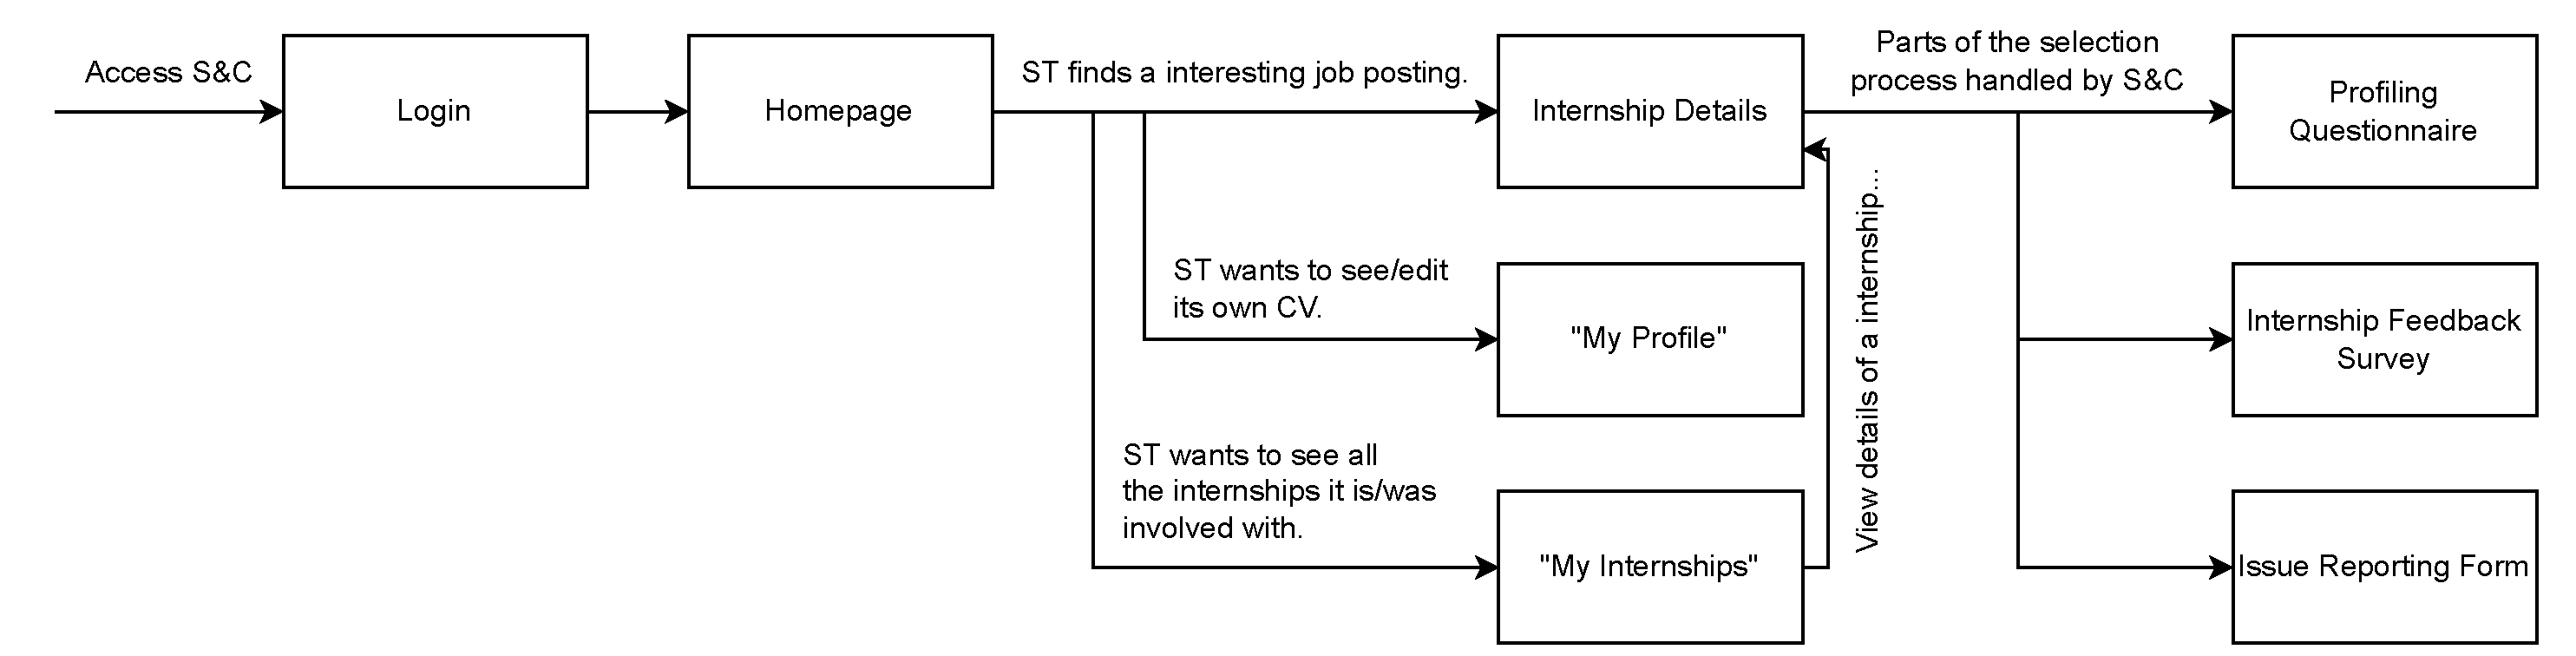
\includegraphics[width=1.0\textwidth]{Images/GUI/ST/Diagram.pdf}
    \caption{ST User Flow Diagram}
    \label{fig:st-user-flow-diagram}
\end{figure}

\par Here is presented the user flow diagram for the ST. The ST uses the Login page to authenticate and access S\&C
and then is redirected to the Homepage. Here the user can discover new internships and view their details
(Internship Details). The Internship Details page will allow the user to apply for the internship, access the
Profiling Questionnaire, reports violations using the Issue Reporting Form and, once the internship is over,
access the Internship Feedback Survey. By using the functions in the header the user can access their own profile
("My Profile"), view all the internships they have interacted with ("My Internships") and log out of the system.

\subsection{Login - ST}
\label{subsec:login-st}%

\begin{figure}[H]
    \centering
    \fbox{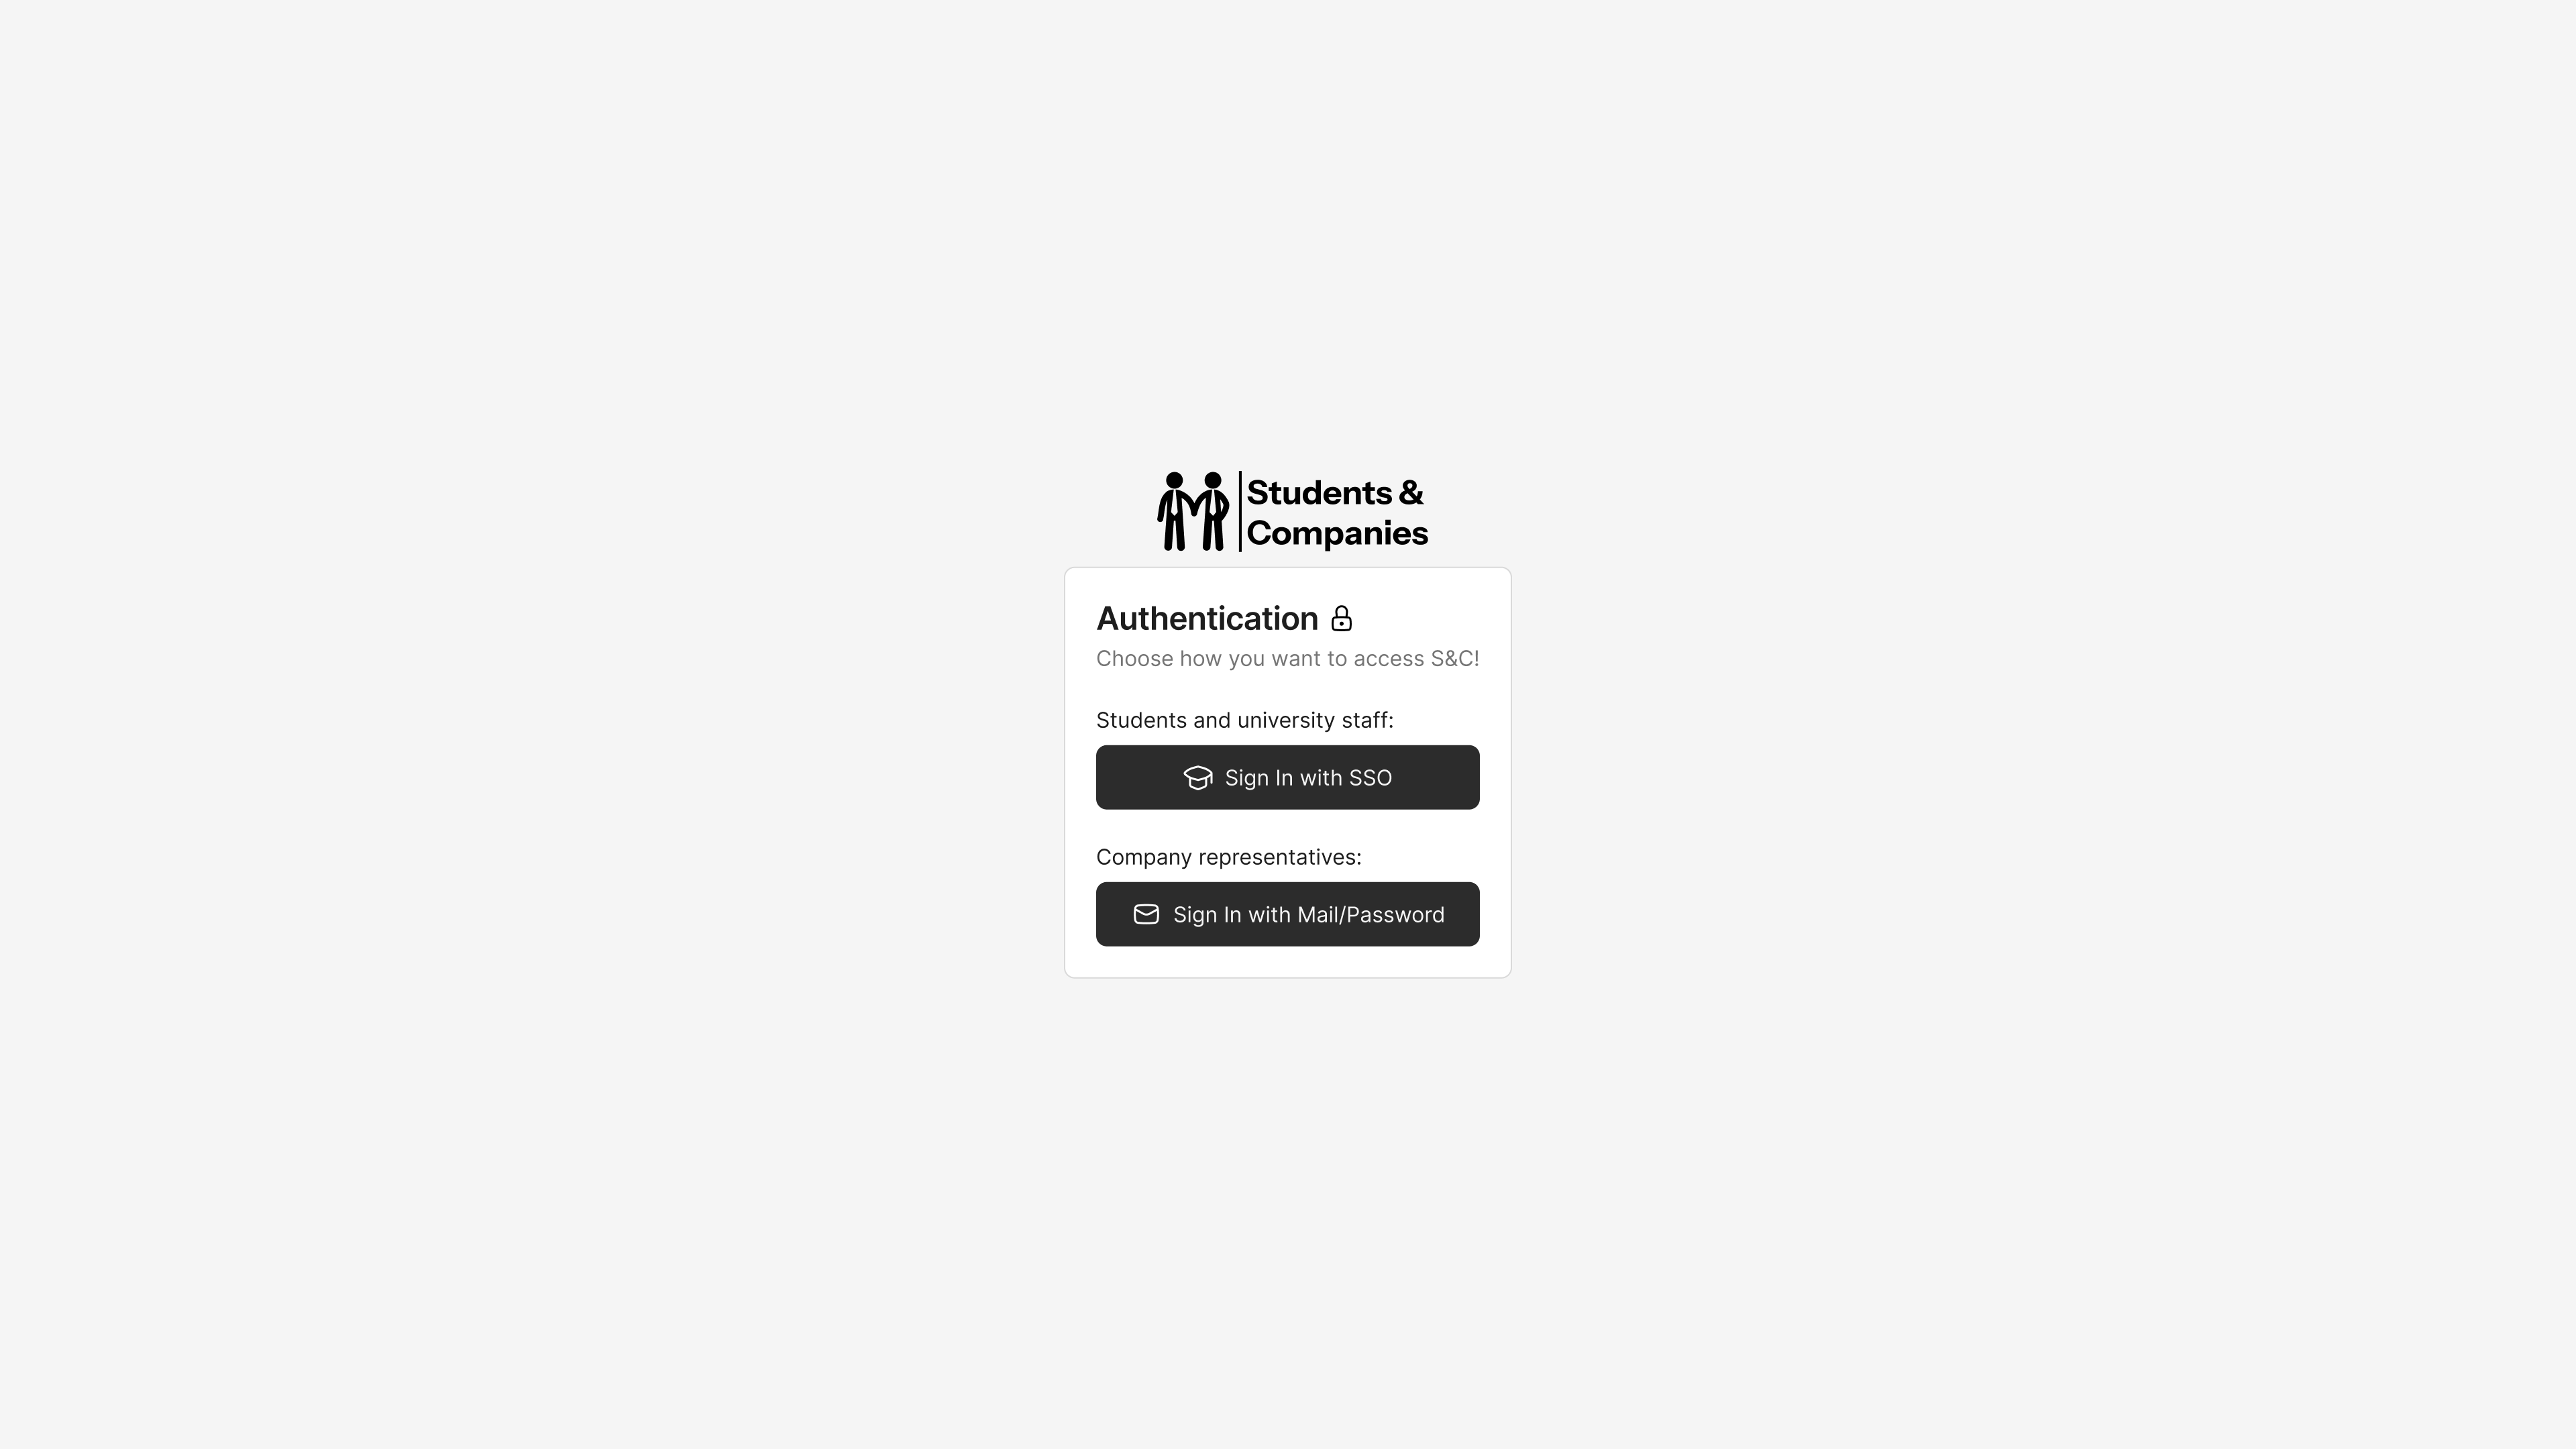
\includegraphics[width=1.0\textwidth]{Images/GUI/ST/Login - ST.png}}
    \caption{Login Page - ST}
    \label{fig:login-page-st}
\end{figure}

\par The login page is the first page the ST will see when accessing the S\&C platform. While ST and UN will use their
university authentication service to log in, a button to use standard credentials is also provided for CO users.

\subsection{Homepage - ST}
\label{subsec:homepage-st}%

\begin{figure}[H]
    \centering
    \fbox{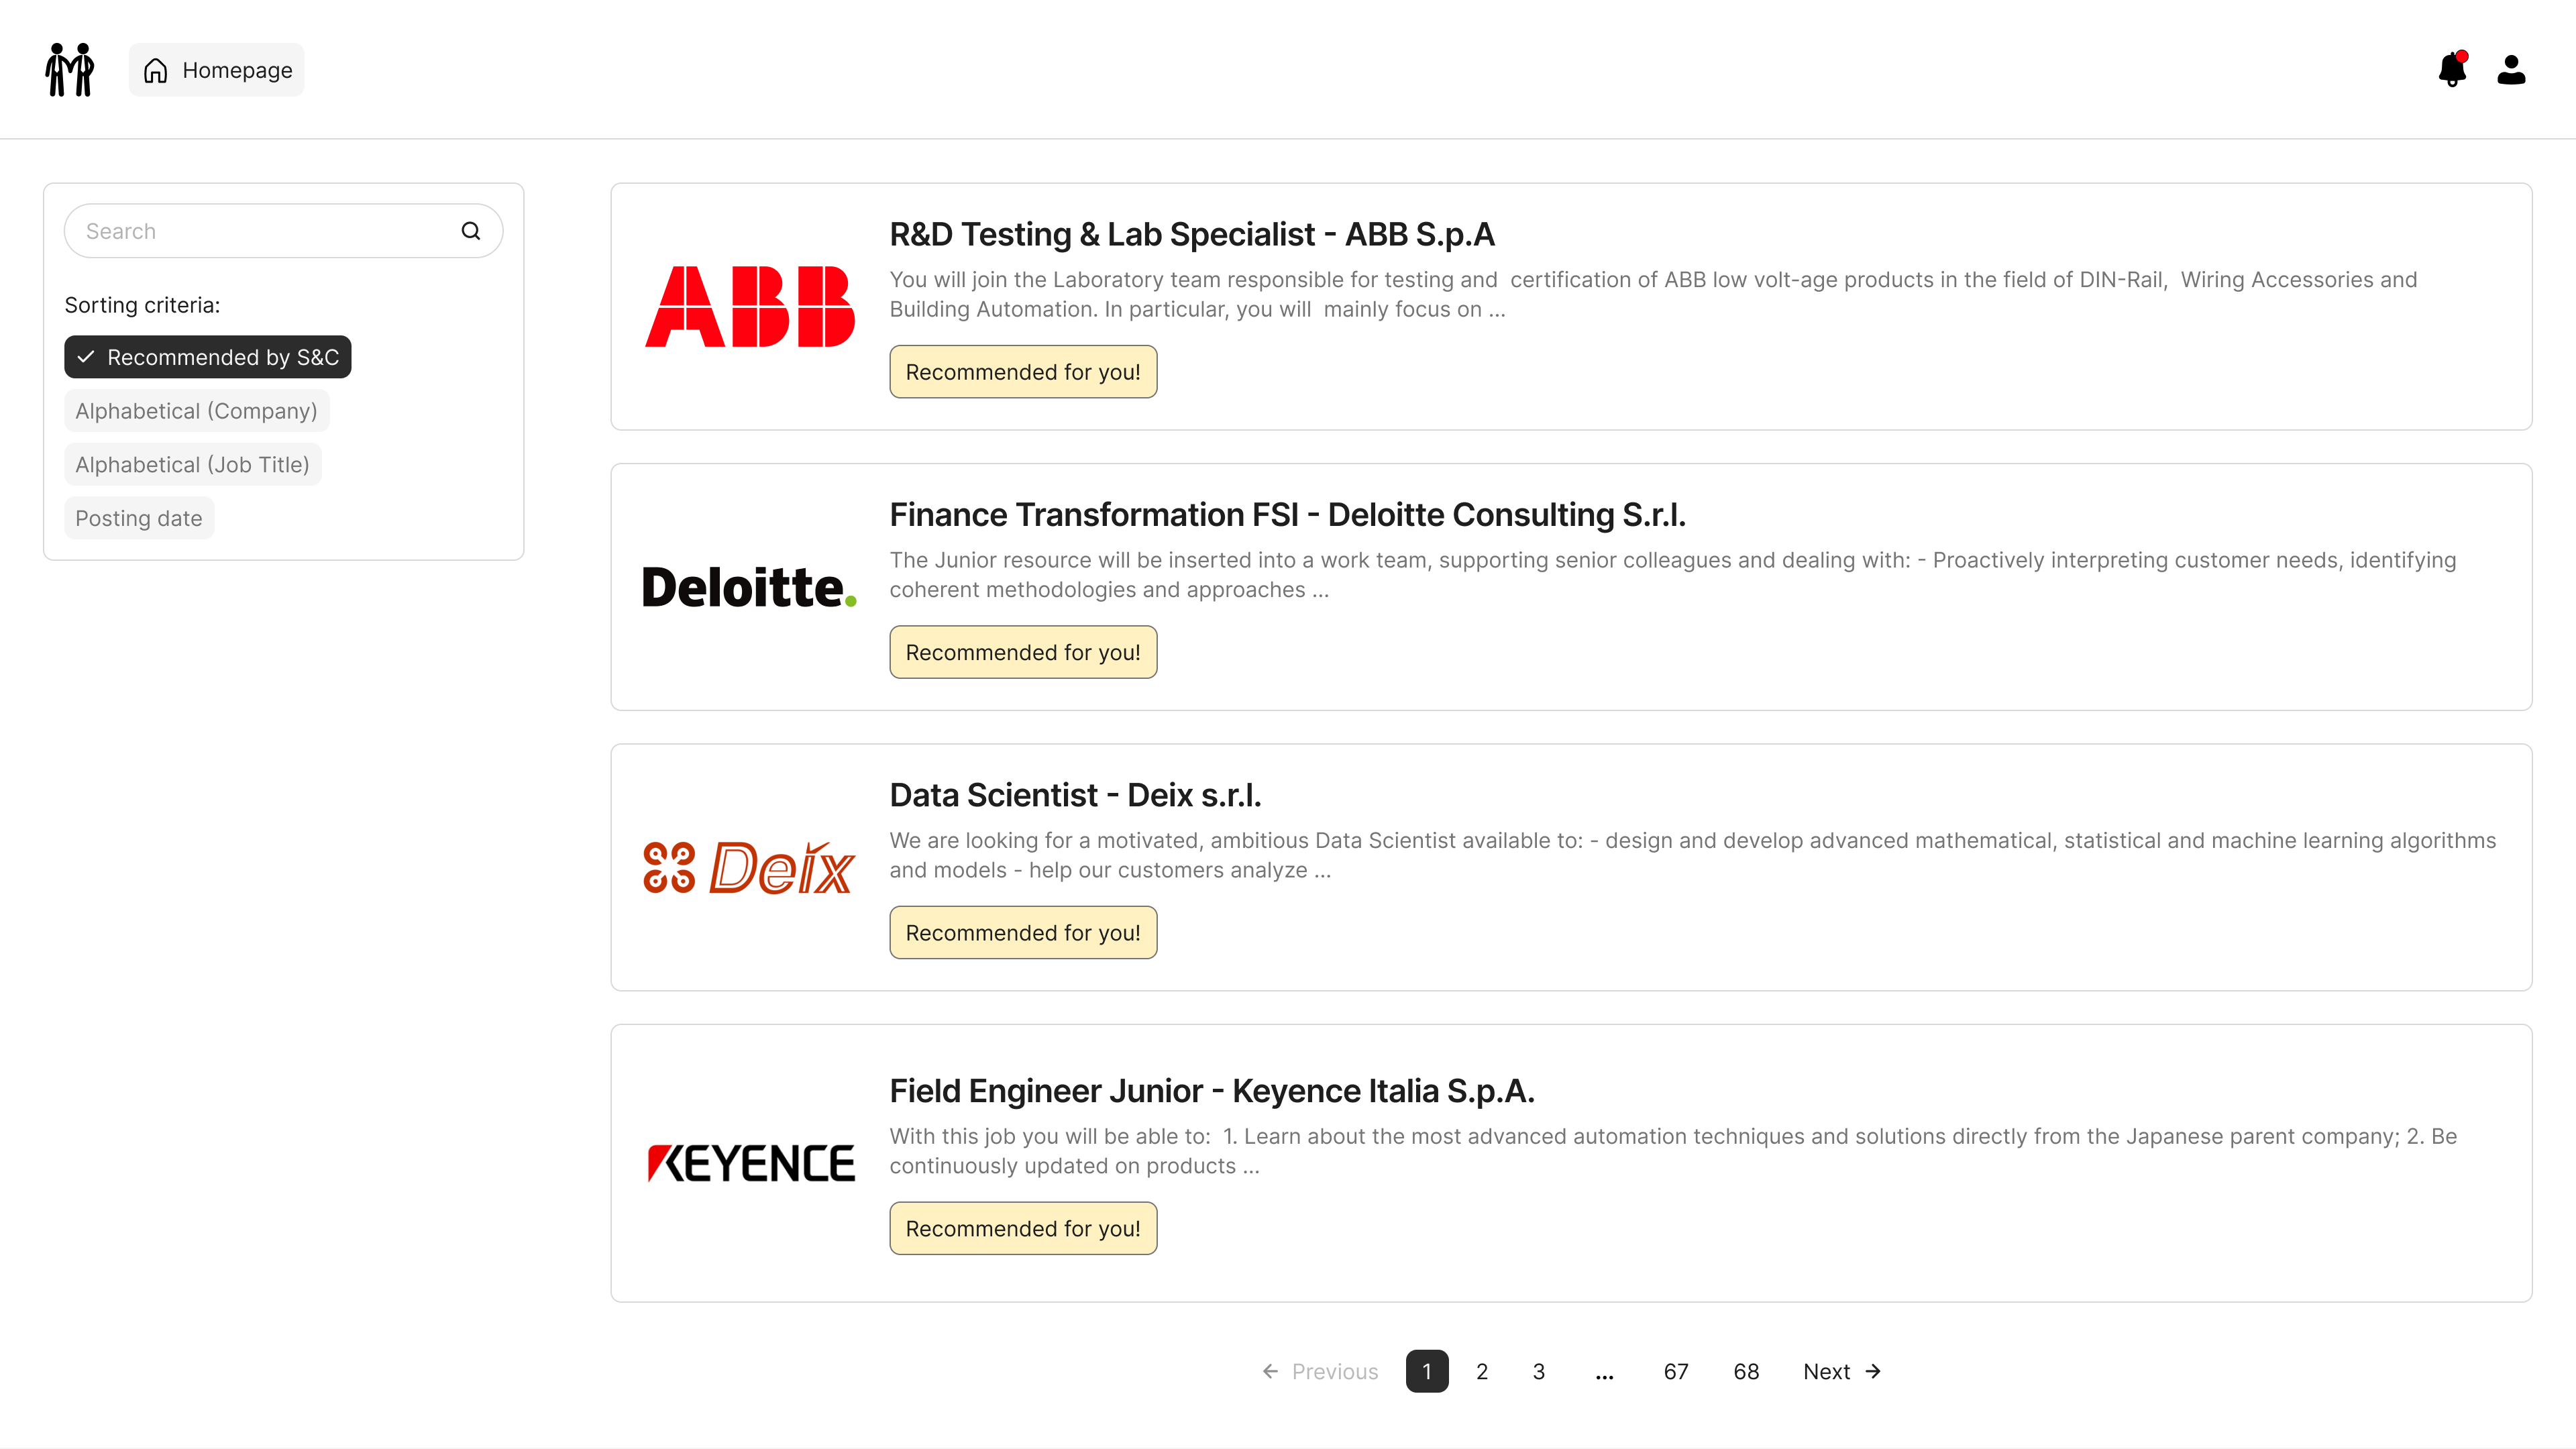
\includegraphics[width=1.0\textwidth]{Images/GUI/ST/Homepage - ST.png}}
    \caption{Homepage - ST}
    \label{fig:homepage-st}
\end{figure}

\par The homepage is the main page for the ST. Here the user can discover new internships and view their details. As
all the other pages, the header is present and allows the user to access their profile, view their internships and
log out. Also, a notification submenu is present to show the user any new notifications in case they missed the email.

\par Appropriate filters are provided to allow the user to search for internships based on their preferences.

\begin{figure}[H]
    \centering
    \fbox{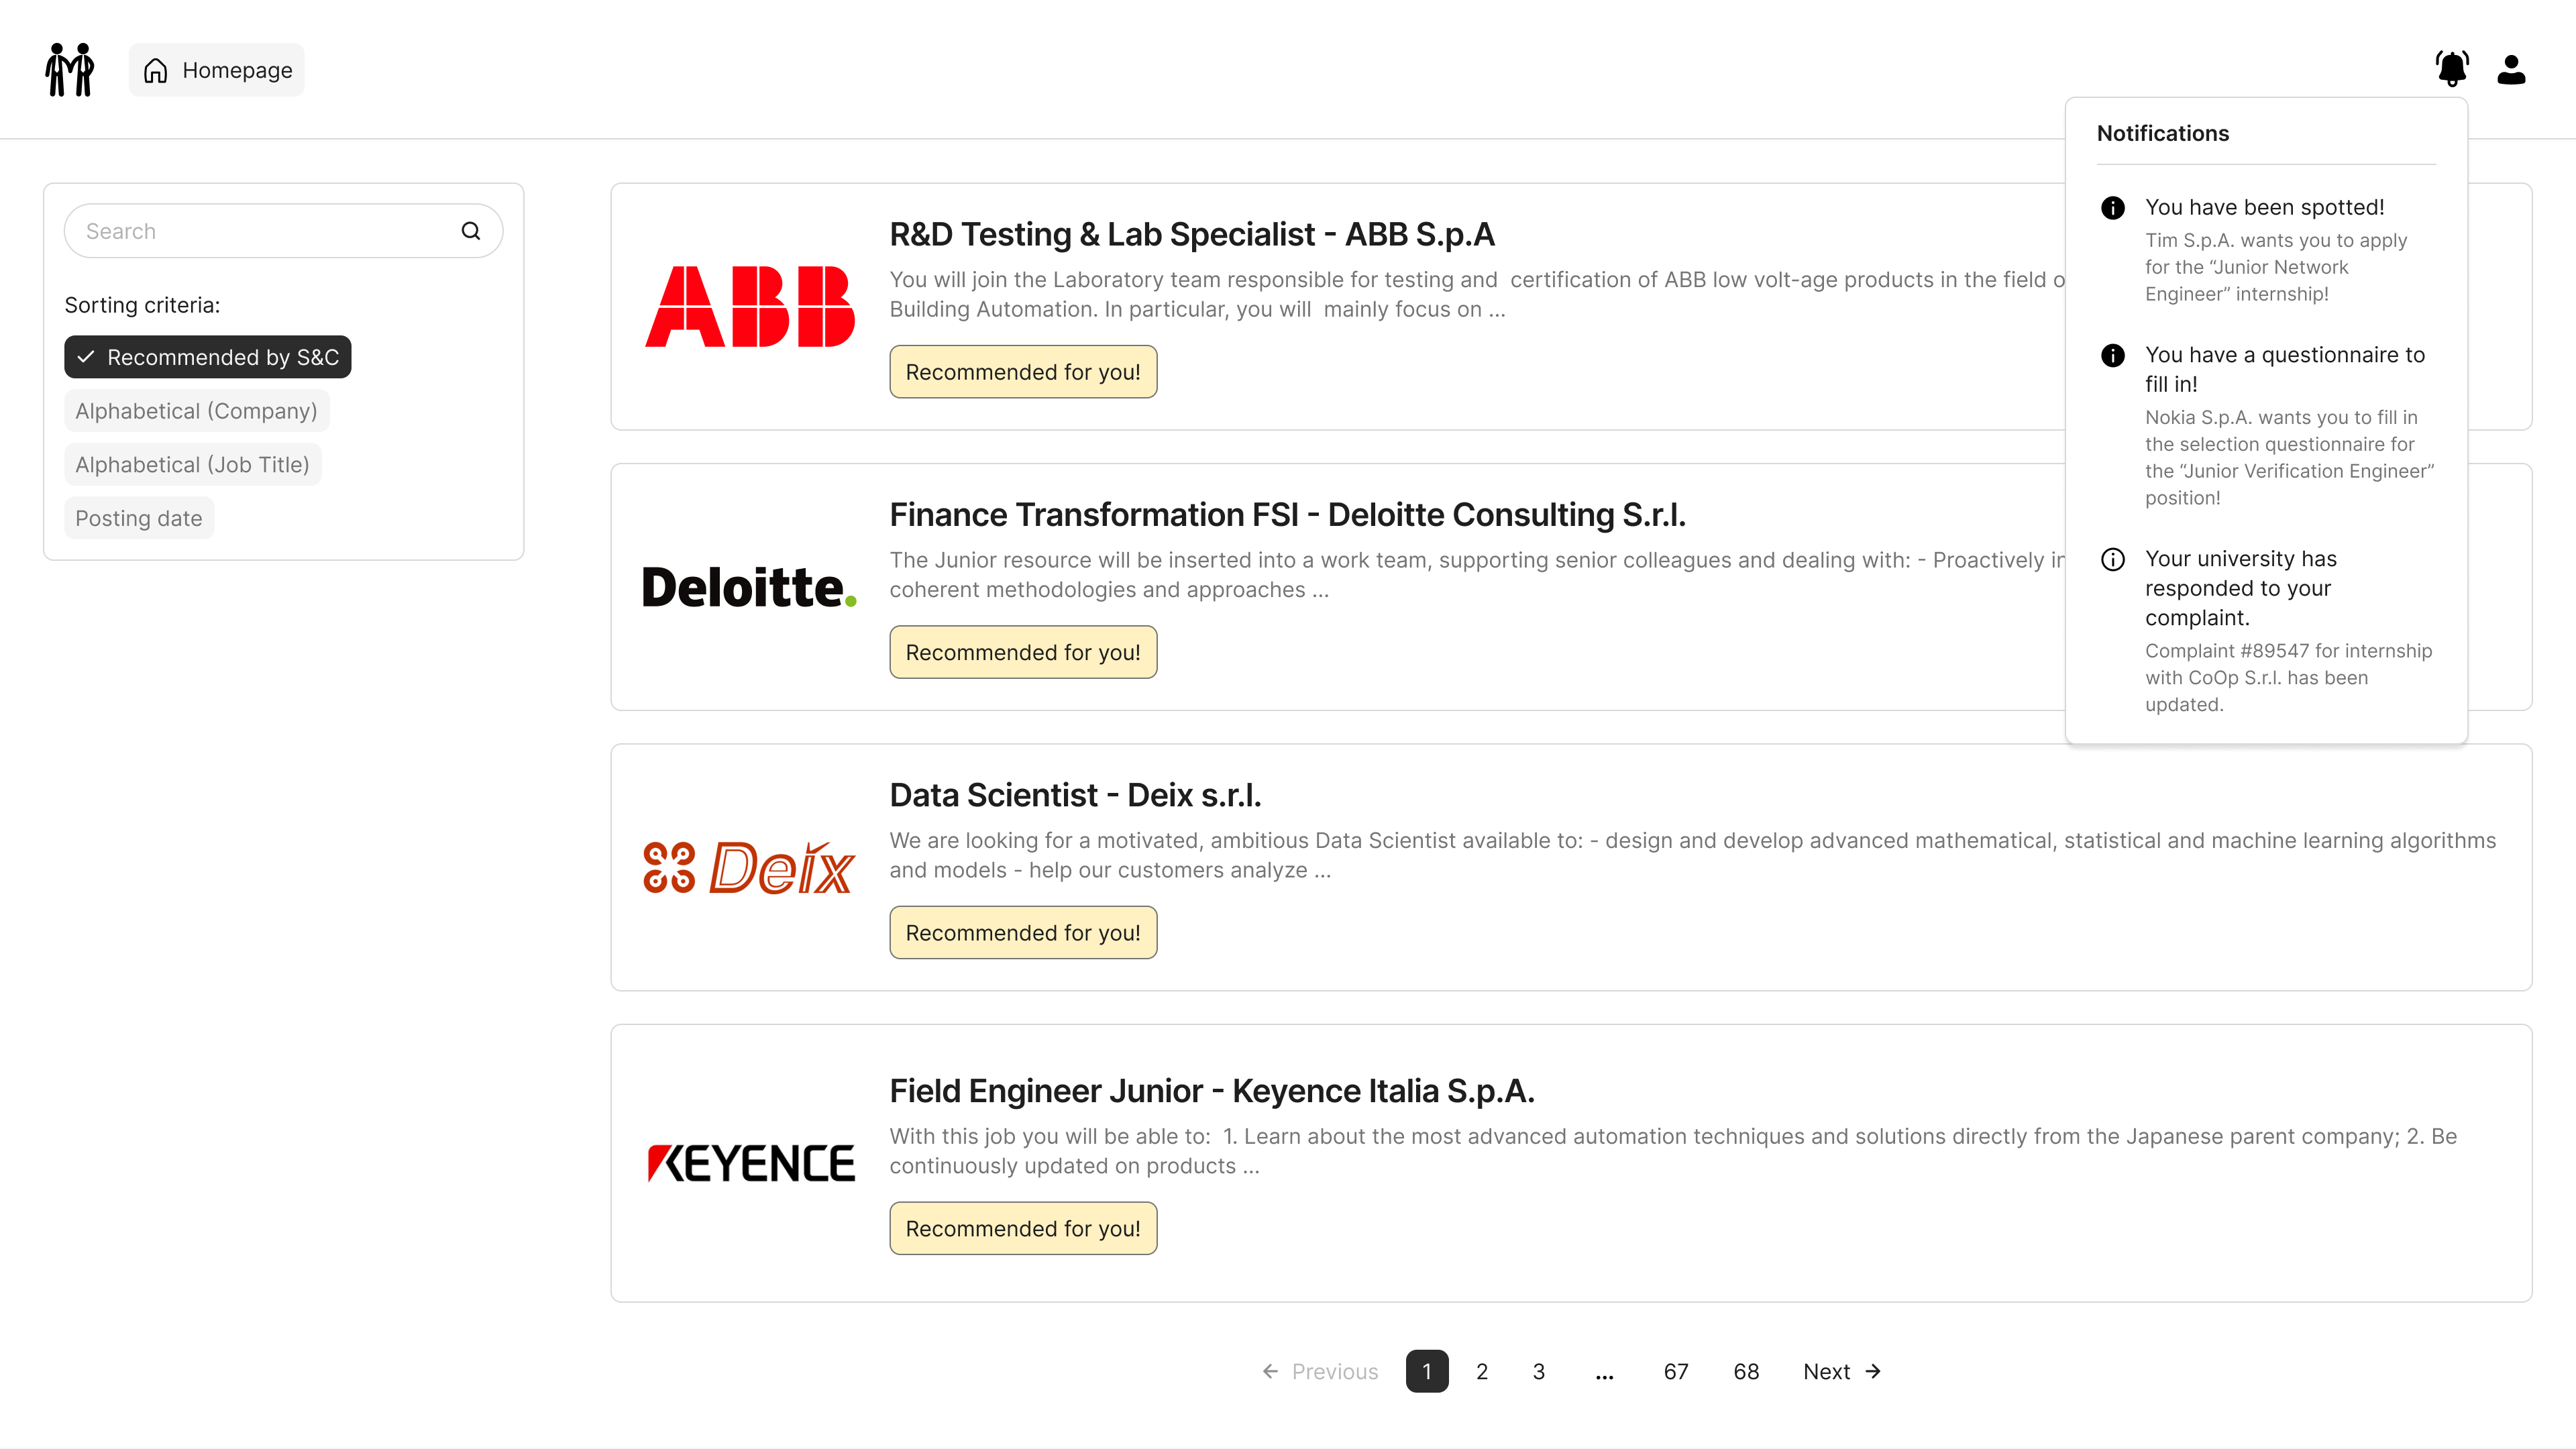
\includegraphics[width=1.0\textwidth]{Images/GUI/ST/Homepage - ST - Notification.png}}
    \caption{Homepage - ST - Notification}
    \label{fig:homepage-st-notification}
\end{figure}

\begin{figure}[H]
    \centering
    \fbox{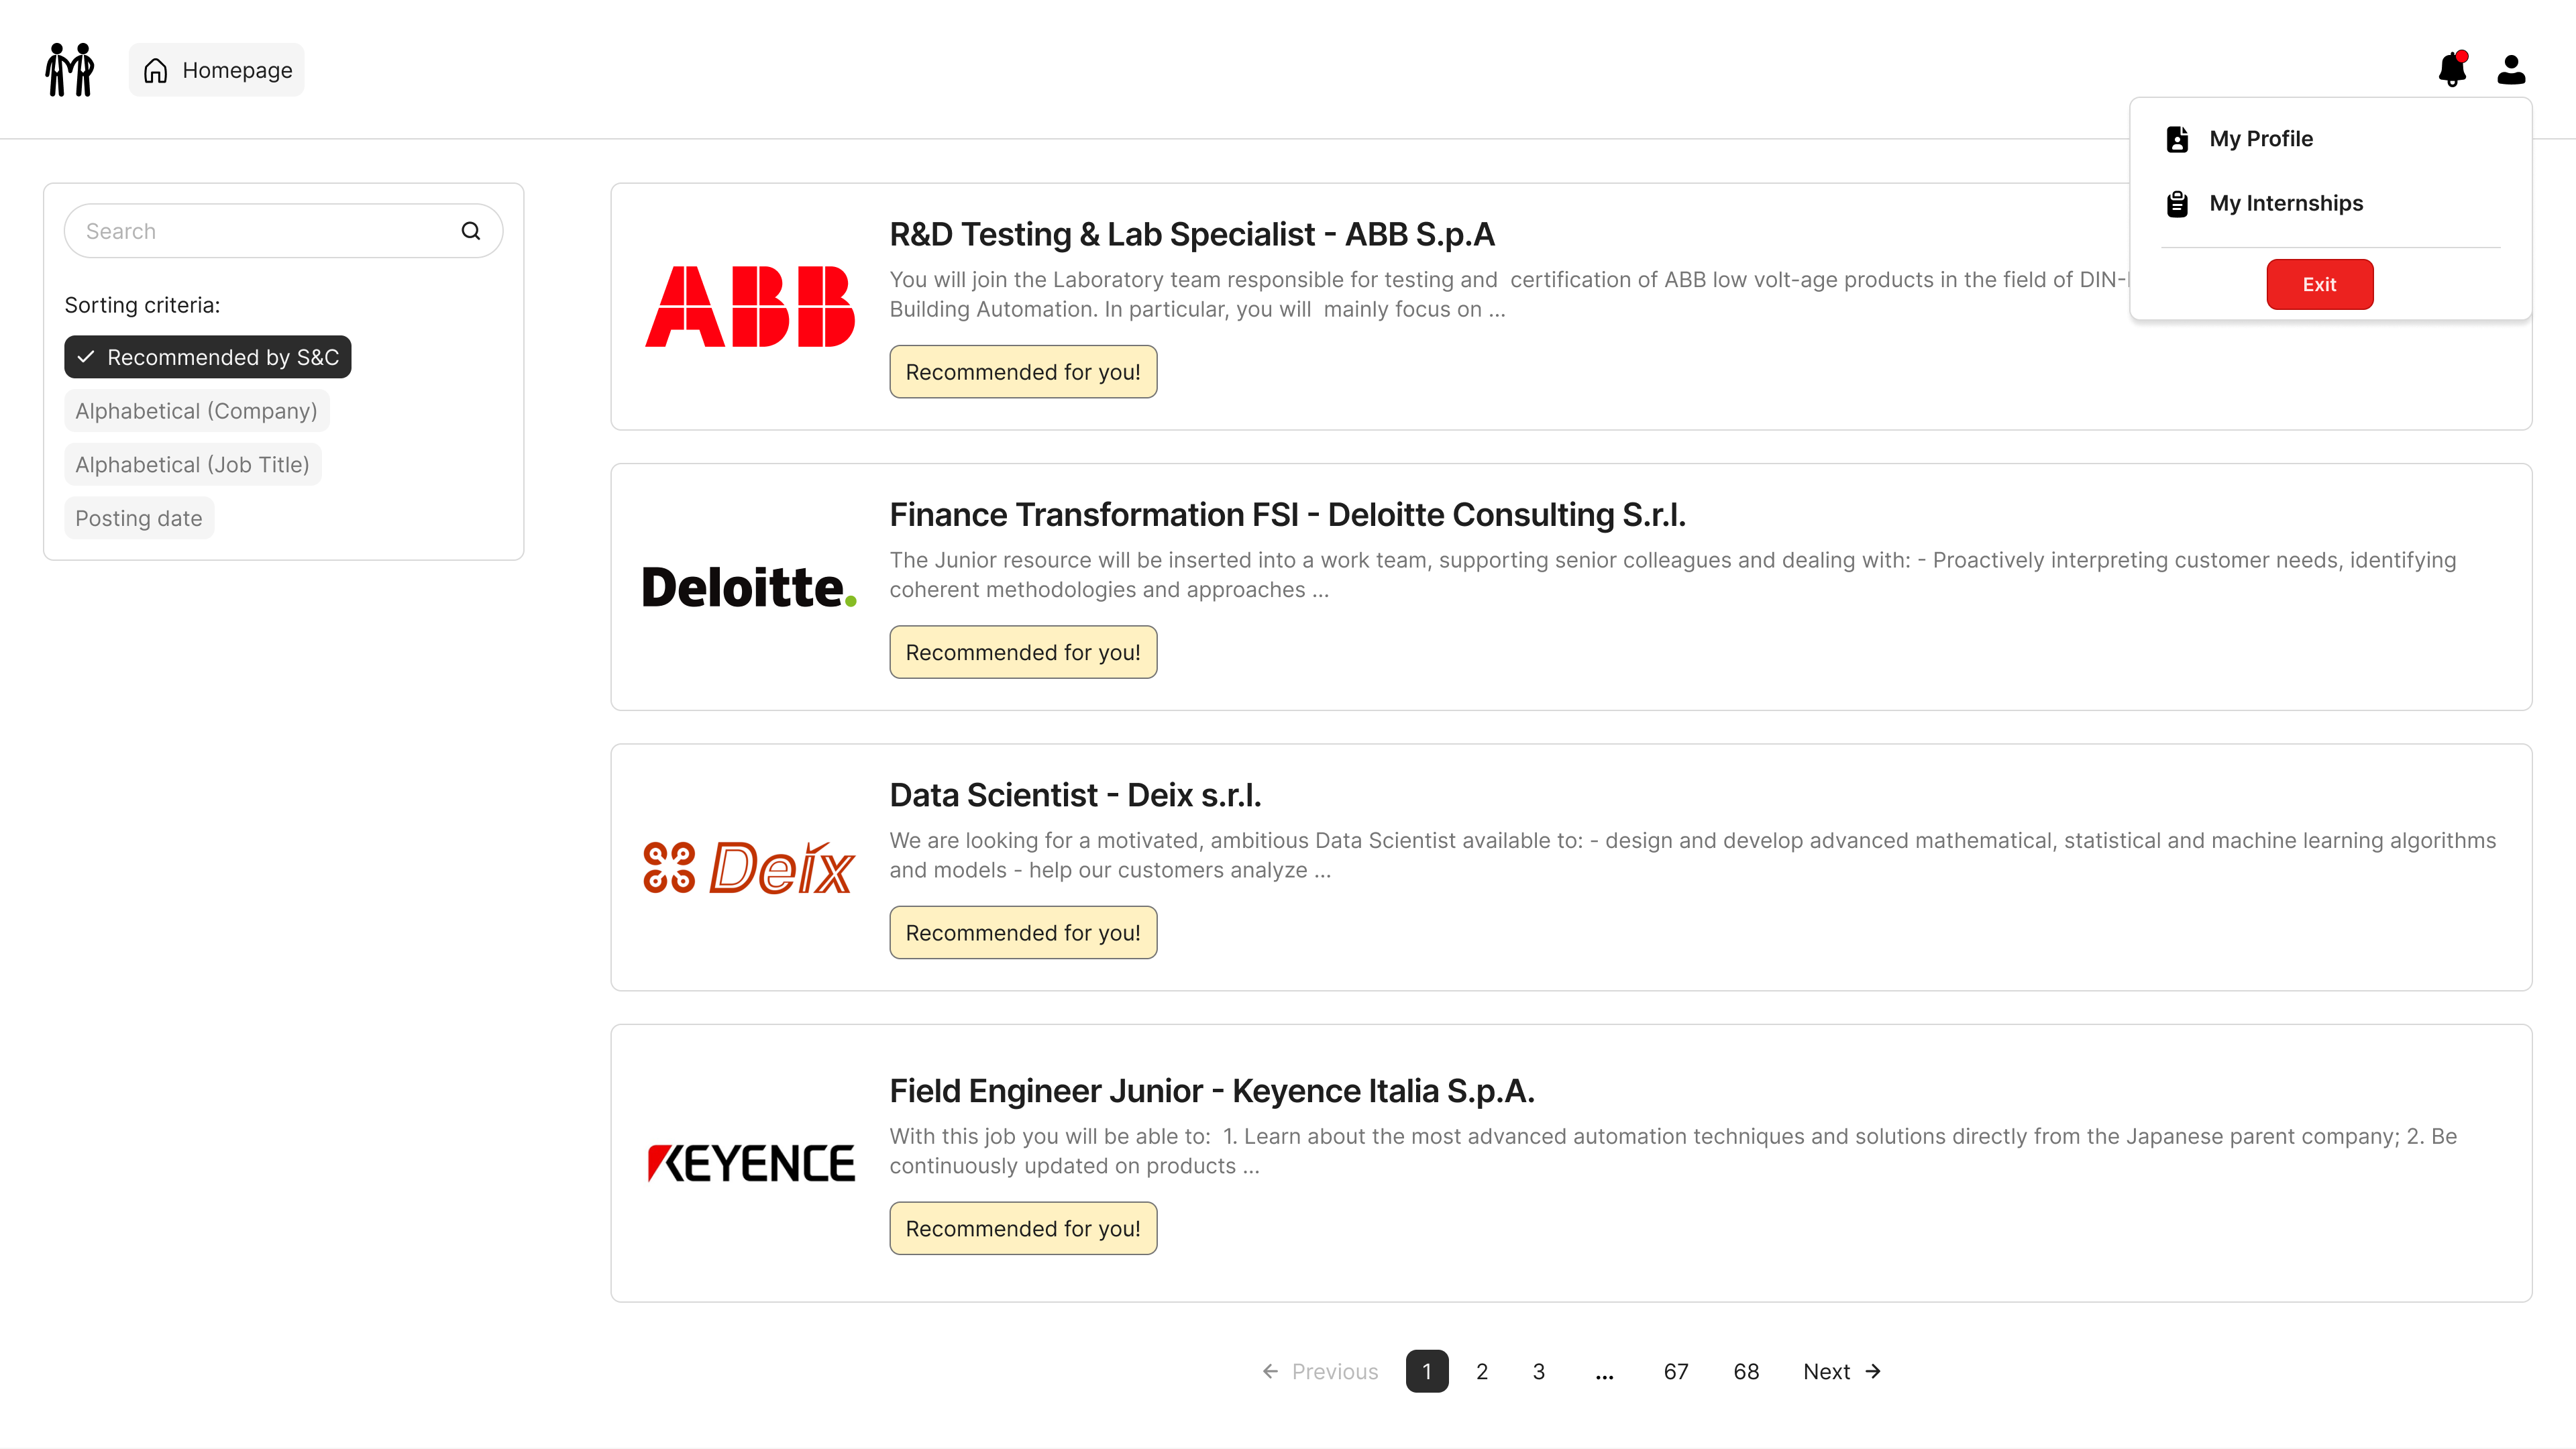
\includegraphics[width=1.0\textwidth]{Images/GUI/ST/Homepage - ST - Profile.png}}
    \caption{Homepage - ST - Profile}
    \label{fig:homepage-st-profile}
\end{figure}

\subsection{"My Internships" - ST}
\label{subsec:my-internships-st}%

\begin{figure}[H]
    \centering
    \fbox{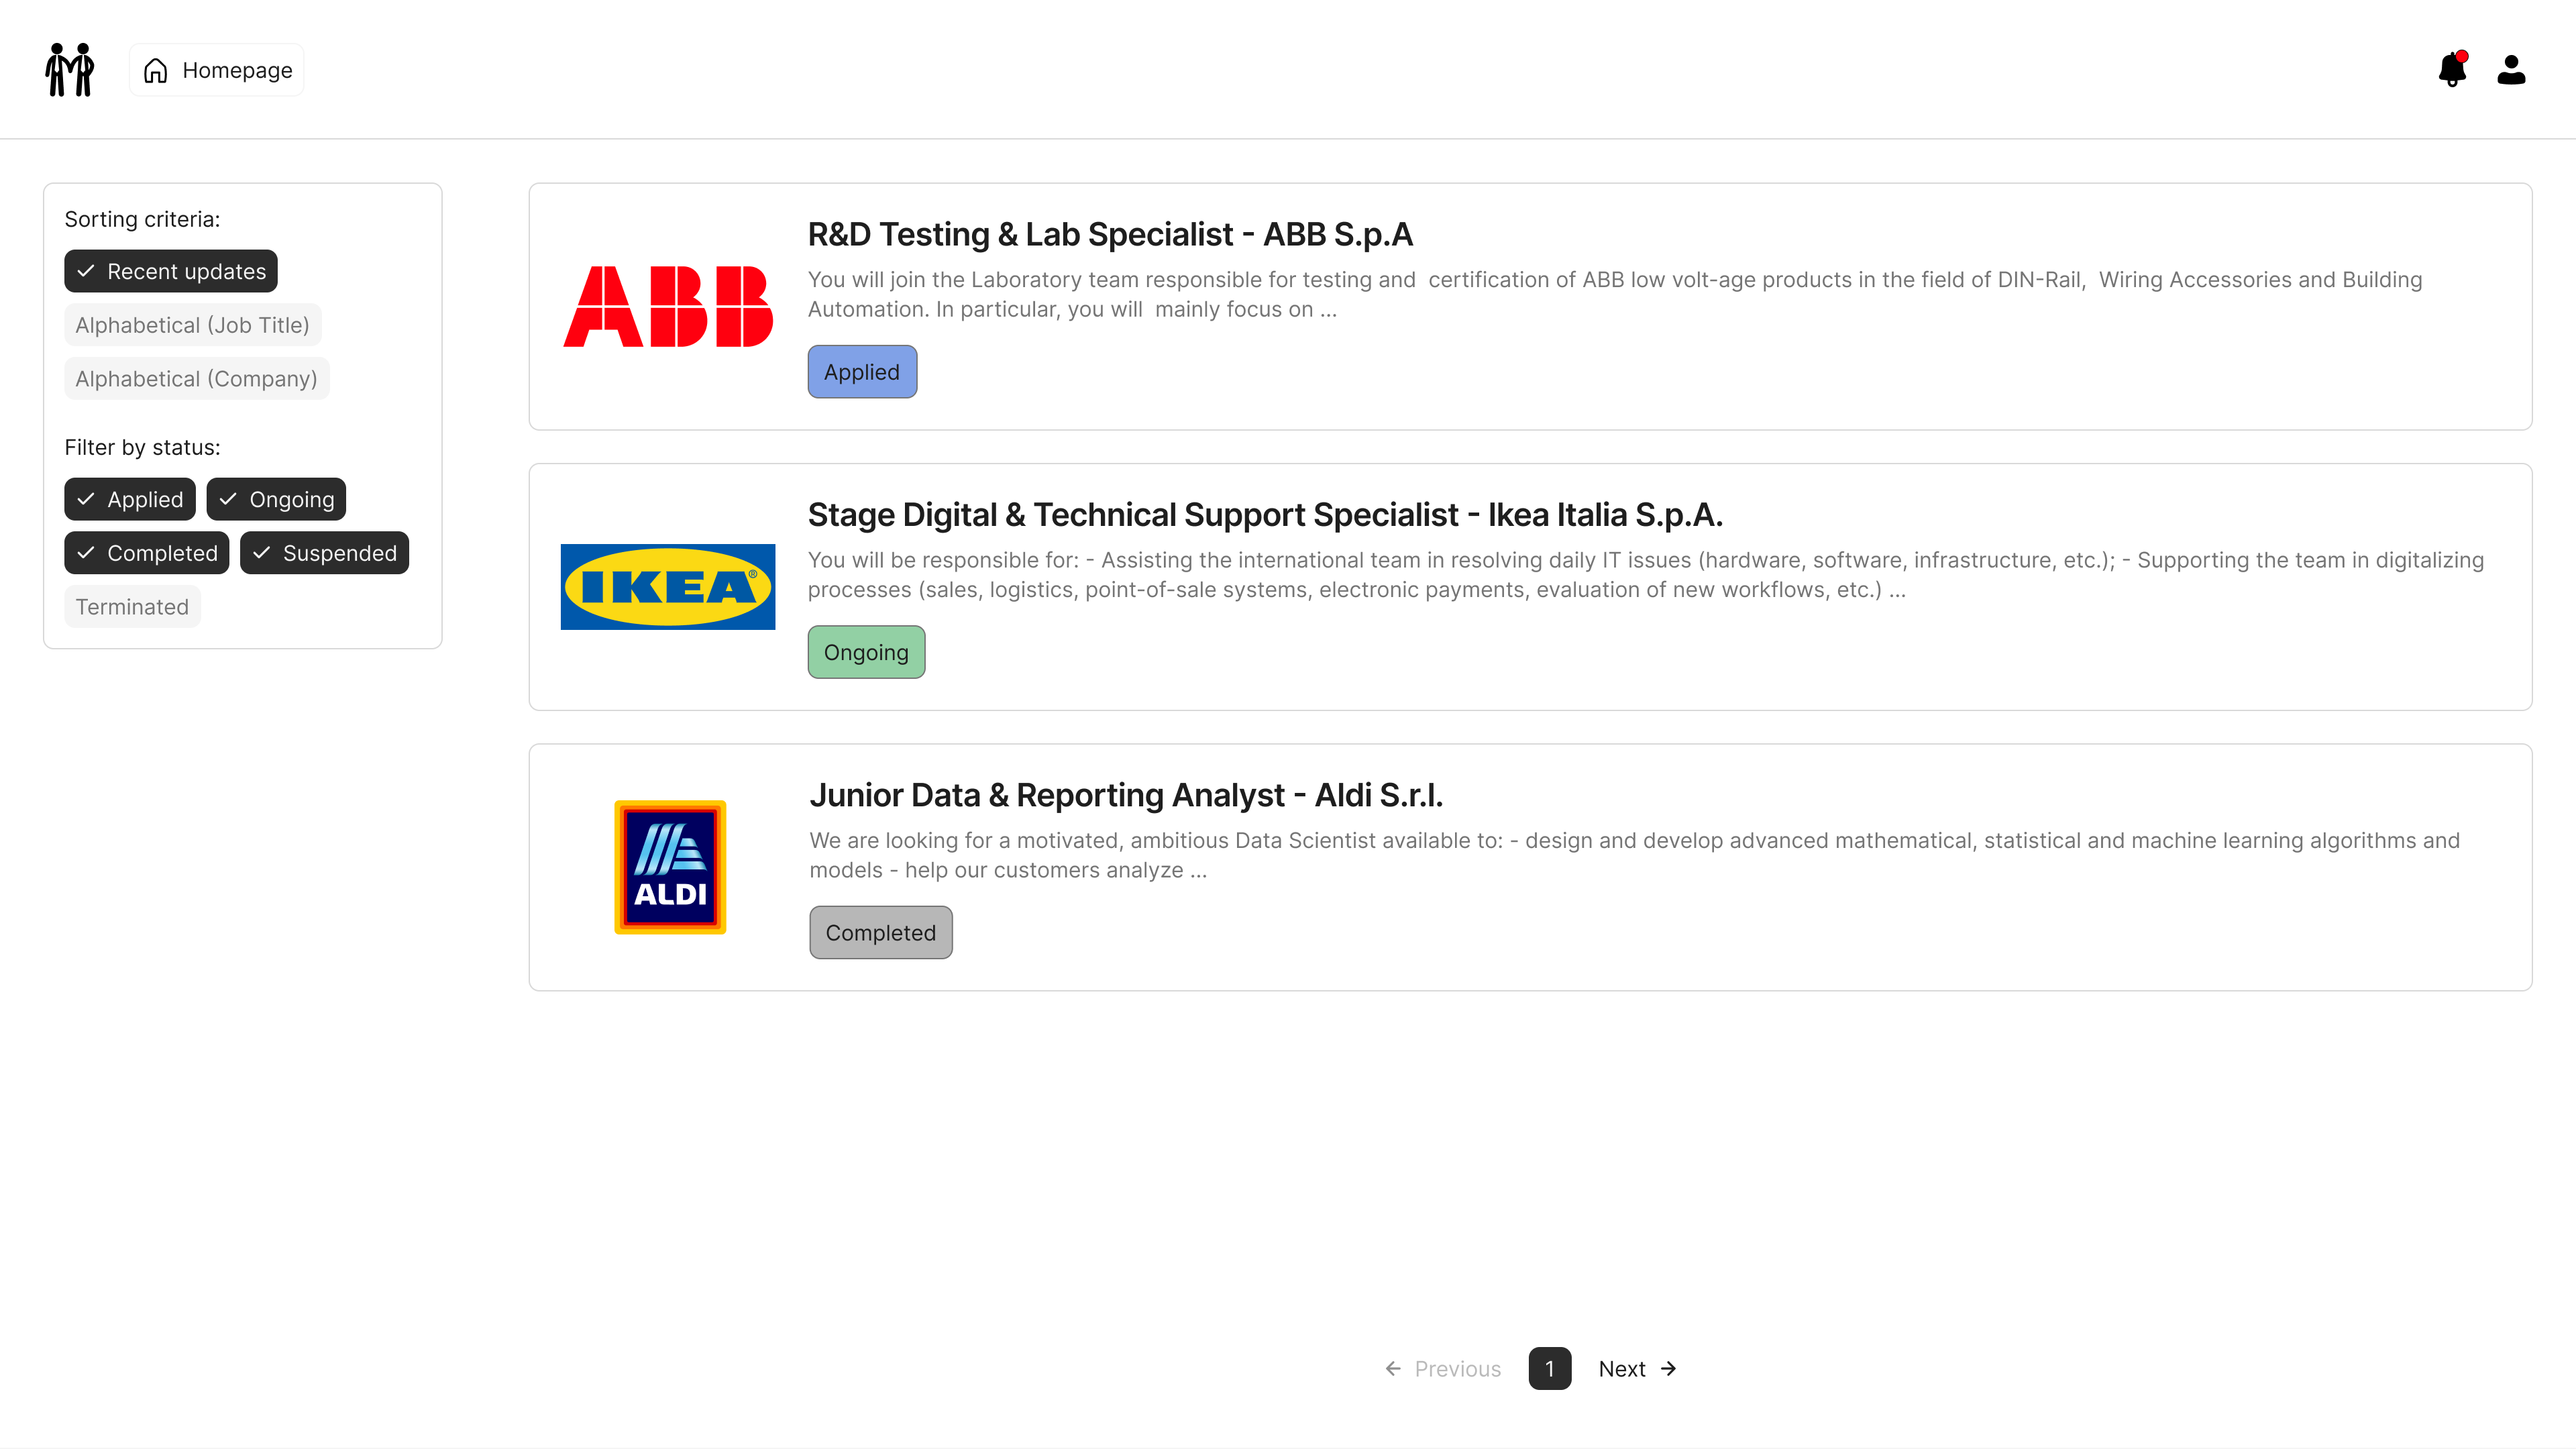
\includegraphics[width=1.0\textwidth]{Images/GUI/ST/My Internships - ST.png}}
    \caption{"My Internships" - ST}
    \label{fig:my-internships-st}
\end{figure}

\par The "My Internships" page allows the ST to view all the internships they have interacted with. It is similar to
the homepage and as such filters are provided.

\subsection{"My Profile" - ST}
\label{subsec:profile-st}%

\begin{figure}[H]
    \centering
    \fbox{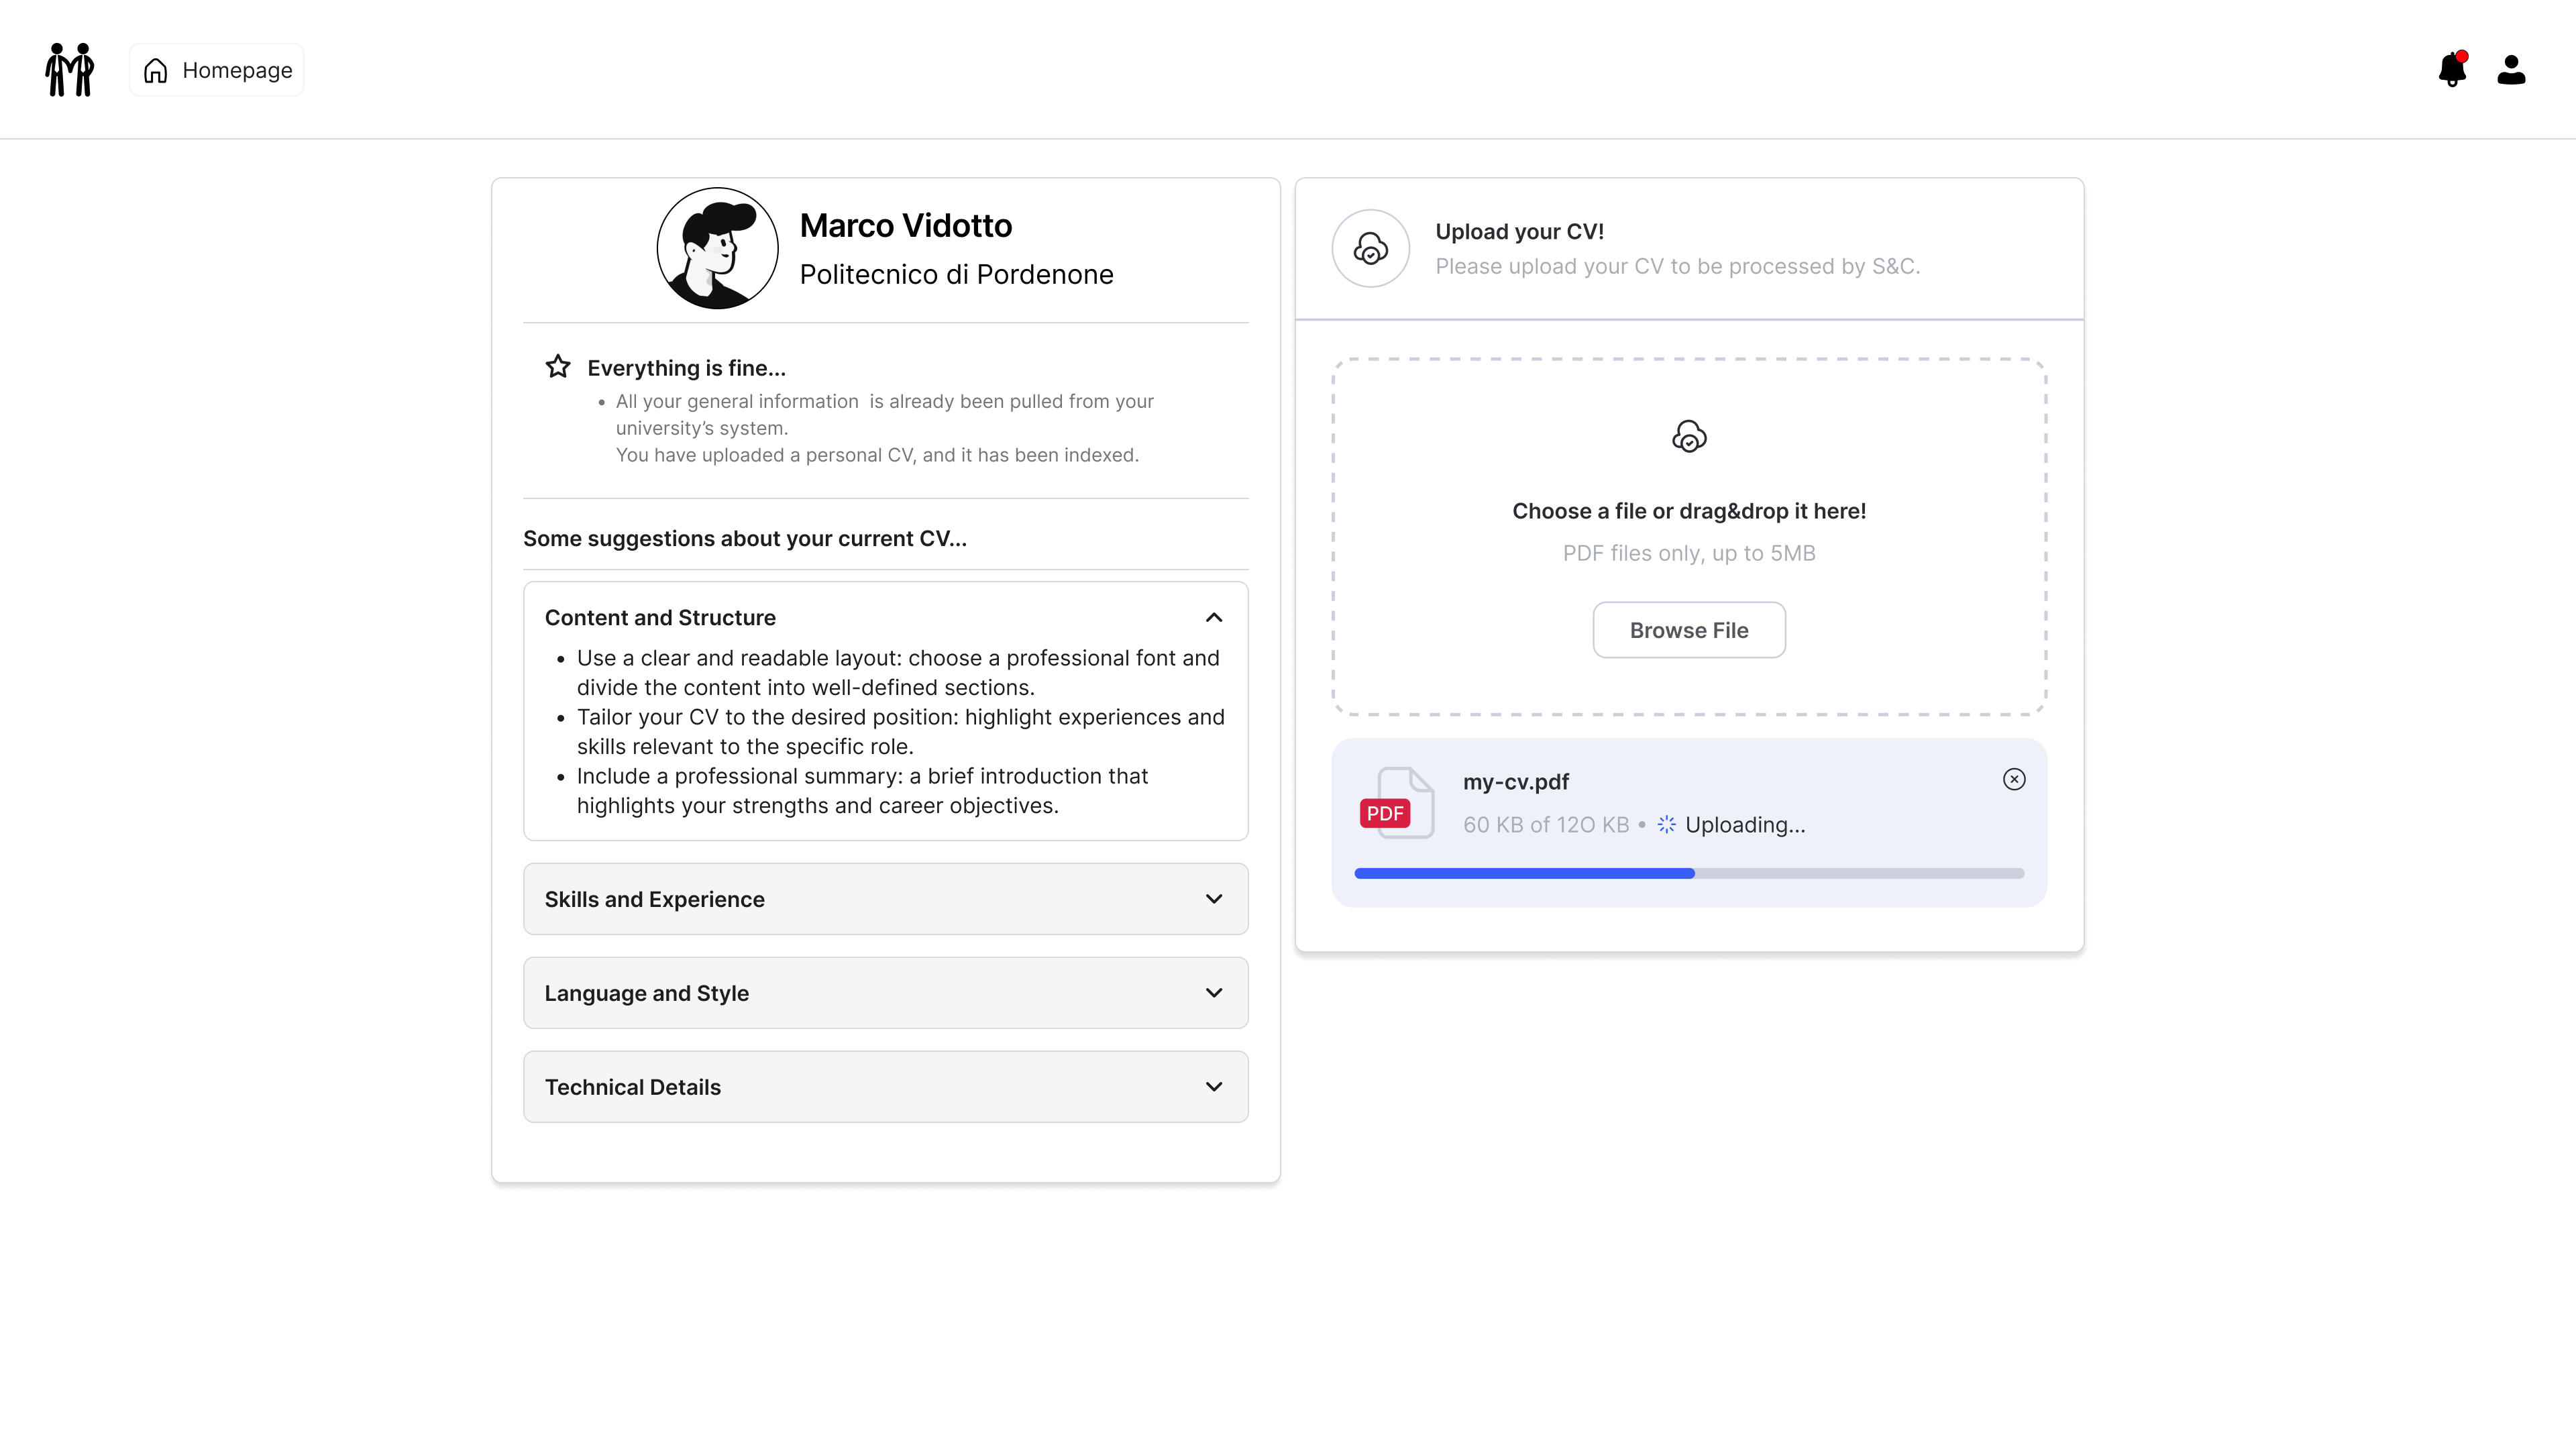
\includegraphics[width=1.0\textwidth]{Images/GUI/ST/Profile - ST.png}}
    \caption{"My Profile" - ST}
    \label{fig:profile-st}
\end{figure}

\par The "My Profile" page allows the ST to update their personal information by uploading a new CV (PDF only!).
Suggestions on how to improve the CV are also provided and will updated based on the processed CV's data.

\subsection{Internship Details - ST}

\begin{figure}[H]
    \centering
    \fbox{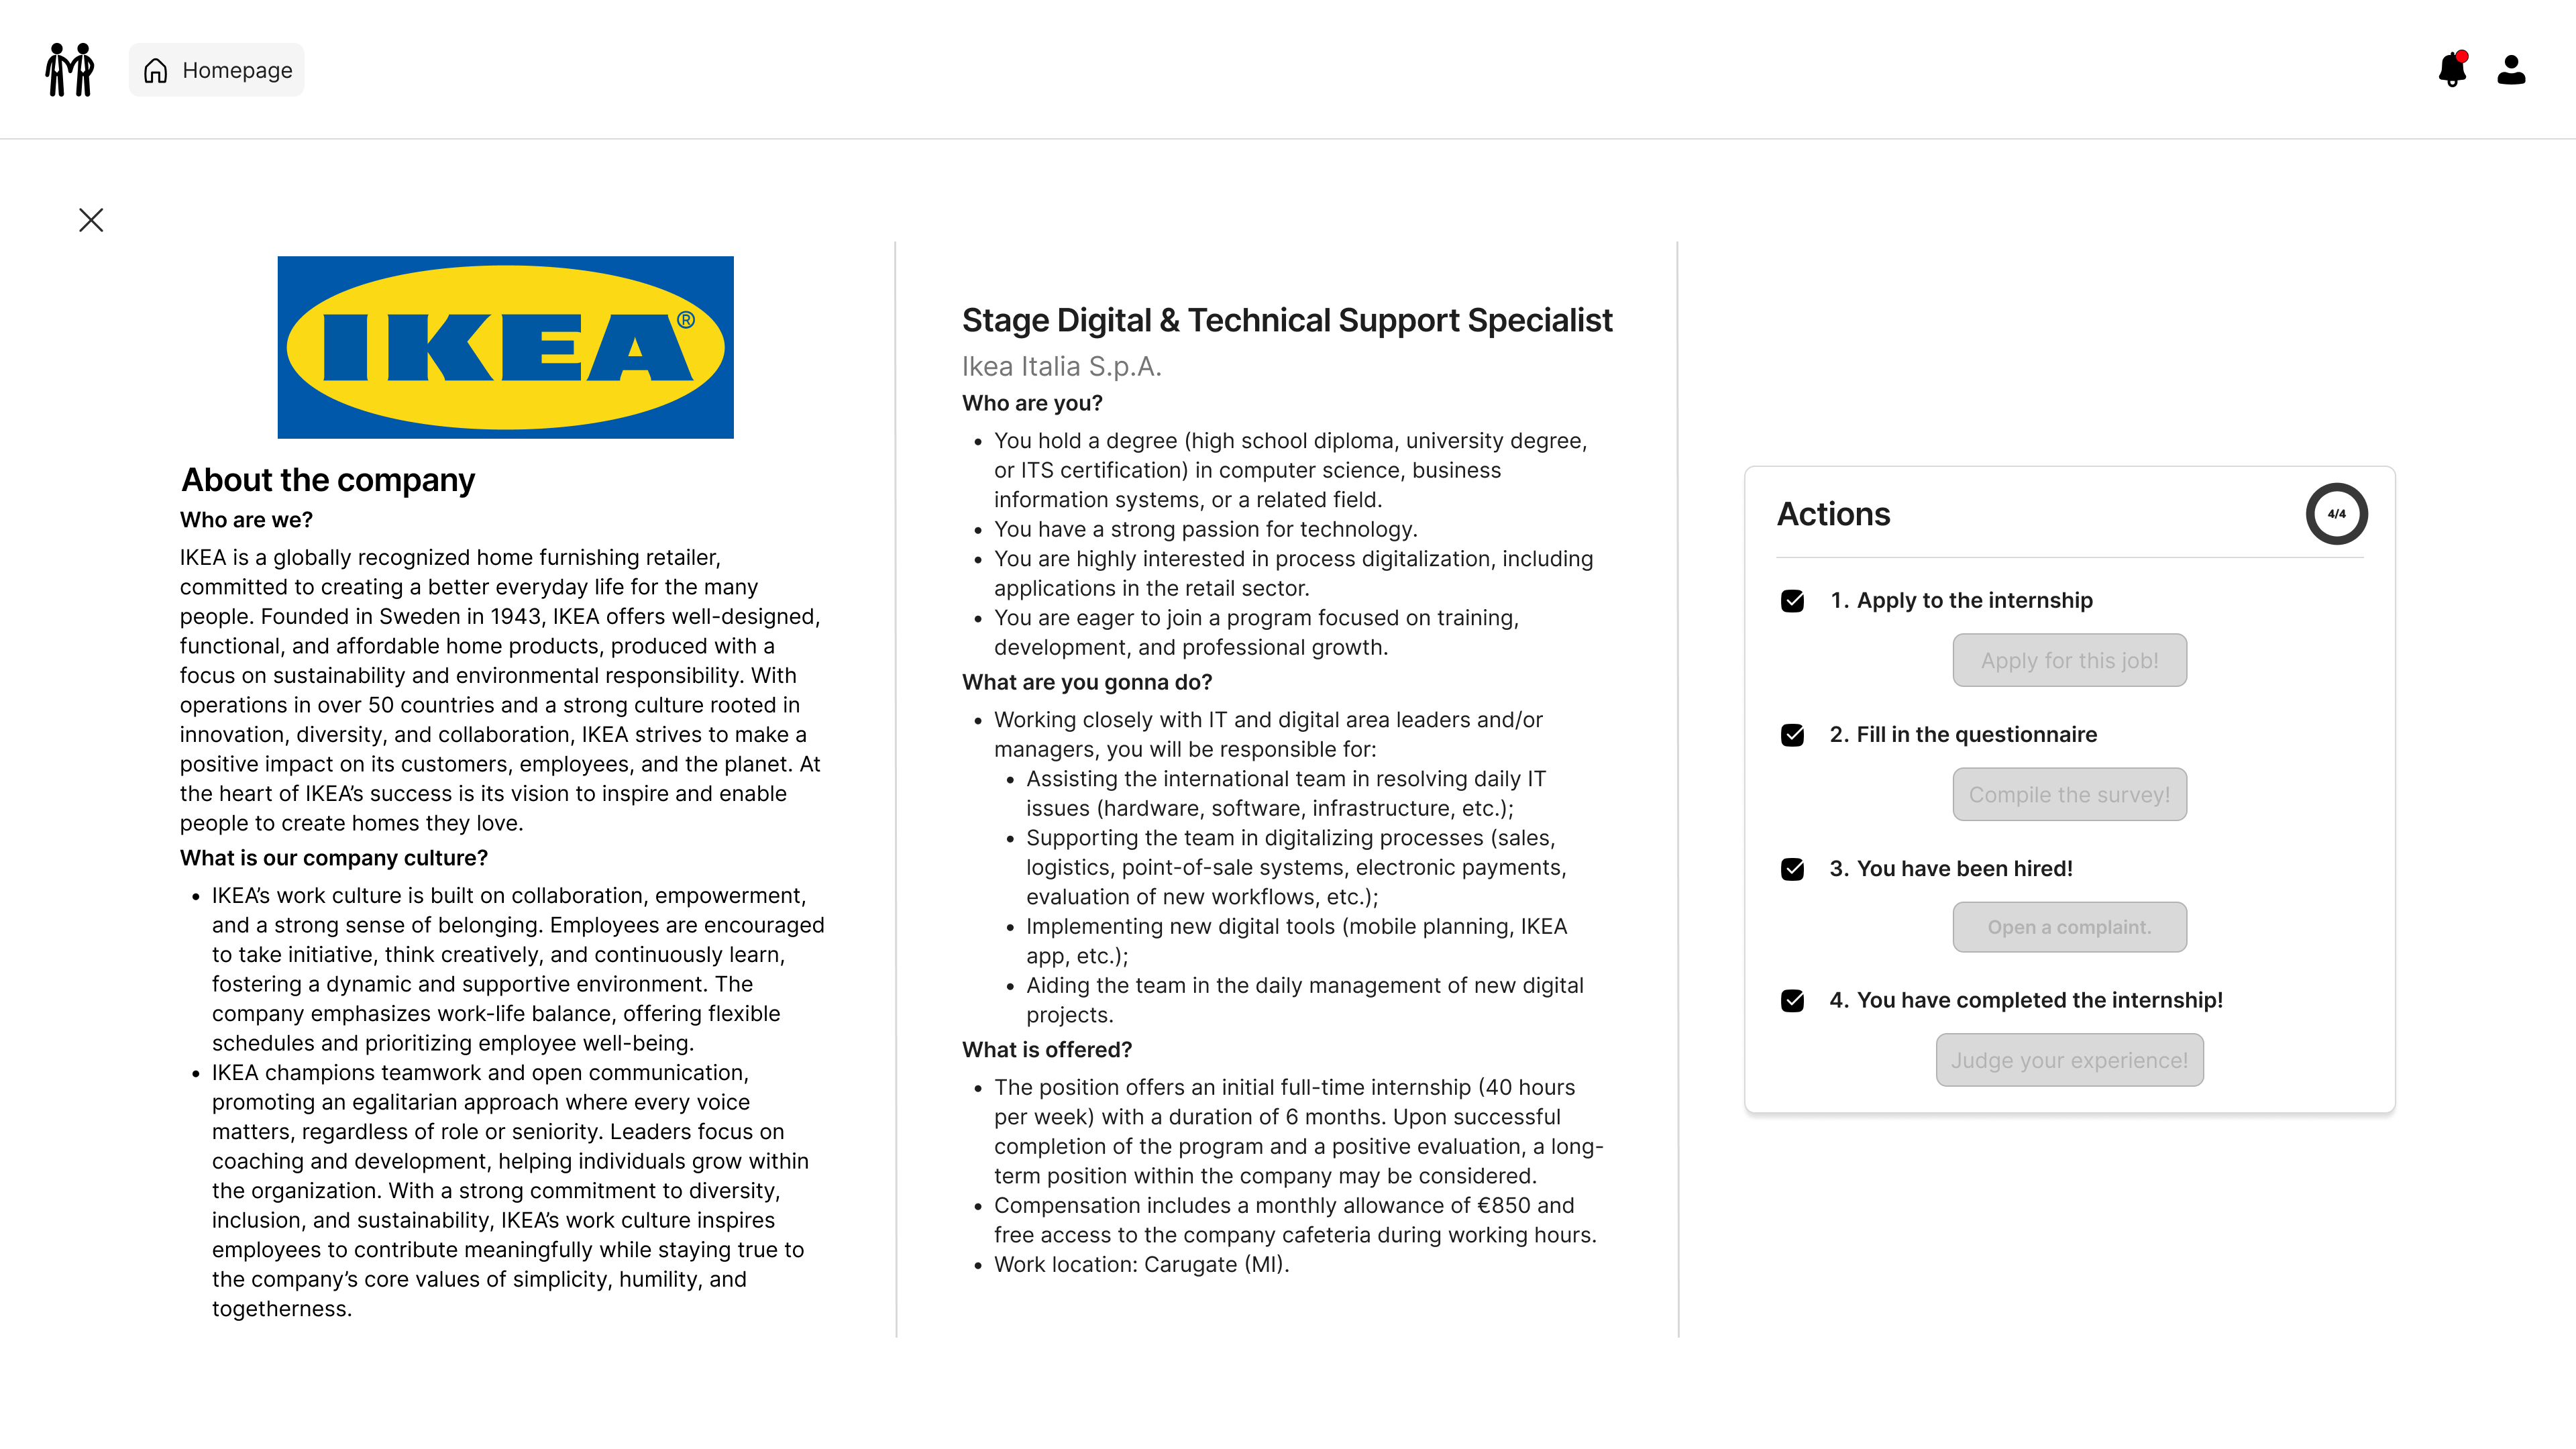
\includegraphics[width=1.0\textwidth]{Images/GUI/ST/Internship Details - Completed - ST.png}}
    \caption{Internship Details - ST}
    \label{fig:internship-details-st}
\end{figure}

\par The Internship Details page allows the ST to view all the details of an internship and the company that is
offering it. The ST can apply for the internship, access the Profiling Questionnaire, report violations using the
Issue Reporting Form and, once the internship is over, access the Internship Feedback Survey.

\par The various functions are enabled or disabled based on the status of the internship. A progress bar is also
present to show the progression of the hiring process.

\par For simplicity, here is presented the page for a completed internship; from this example will it be easy to infer
how the page will look like for all the various stages of the hiring process.

\subsection{Profiling Questionnaire - ST}
\label{subsec:profiling-questionnaire-st}%

\begin{figure}[H]
    \centering
    \fbox{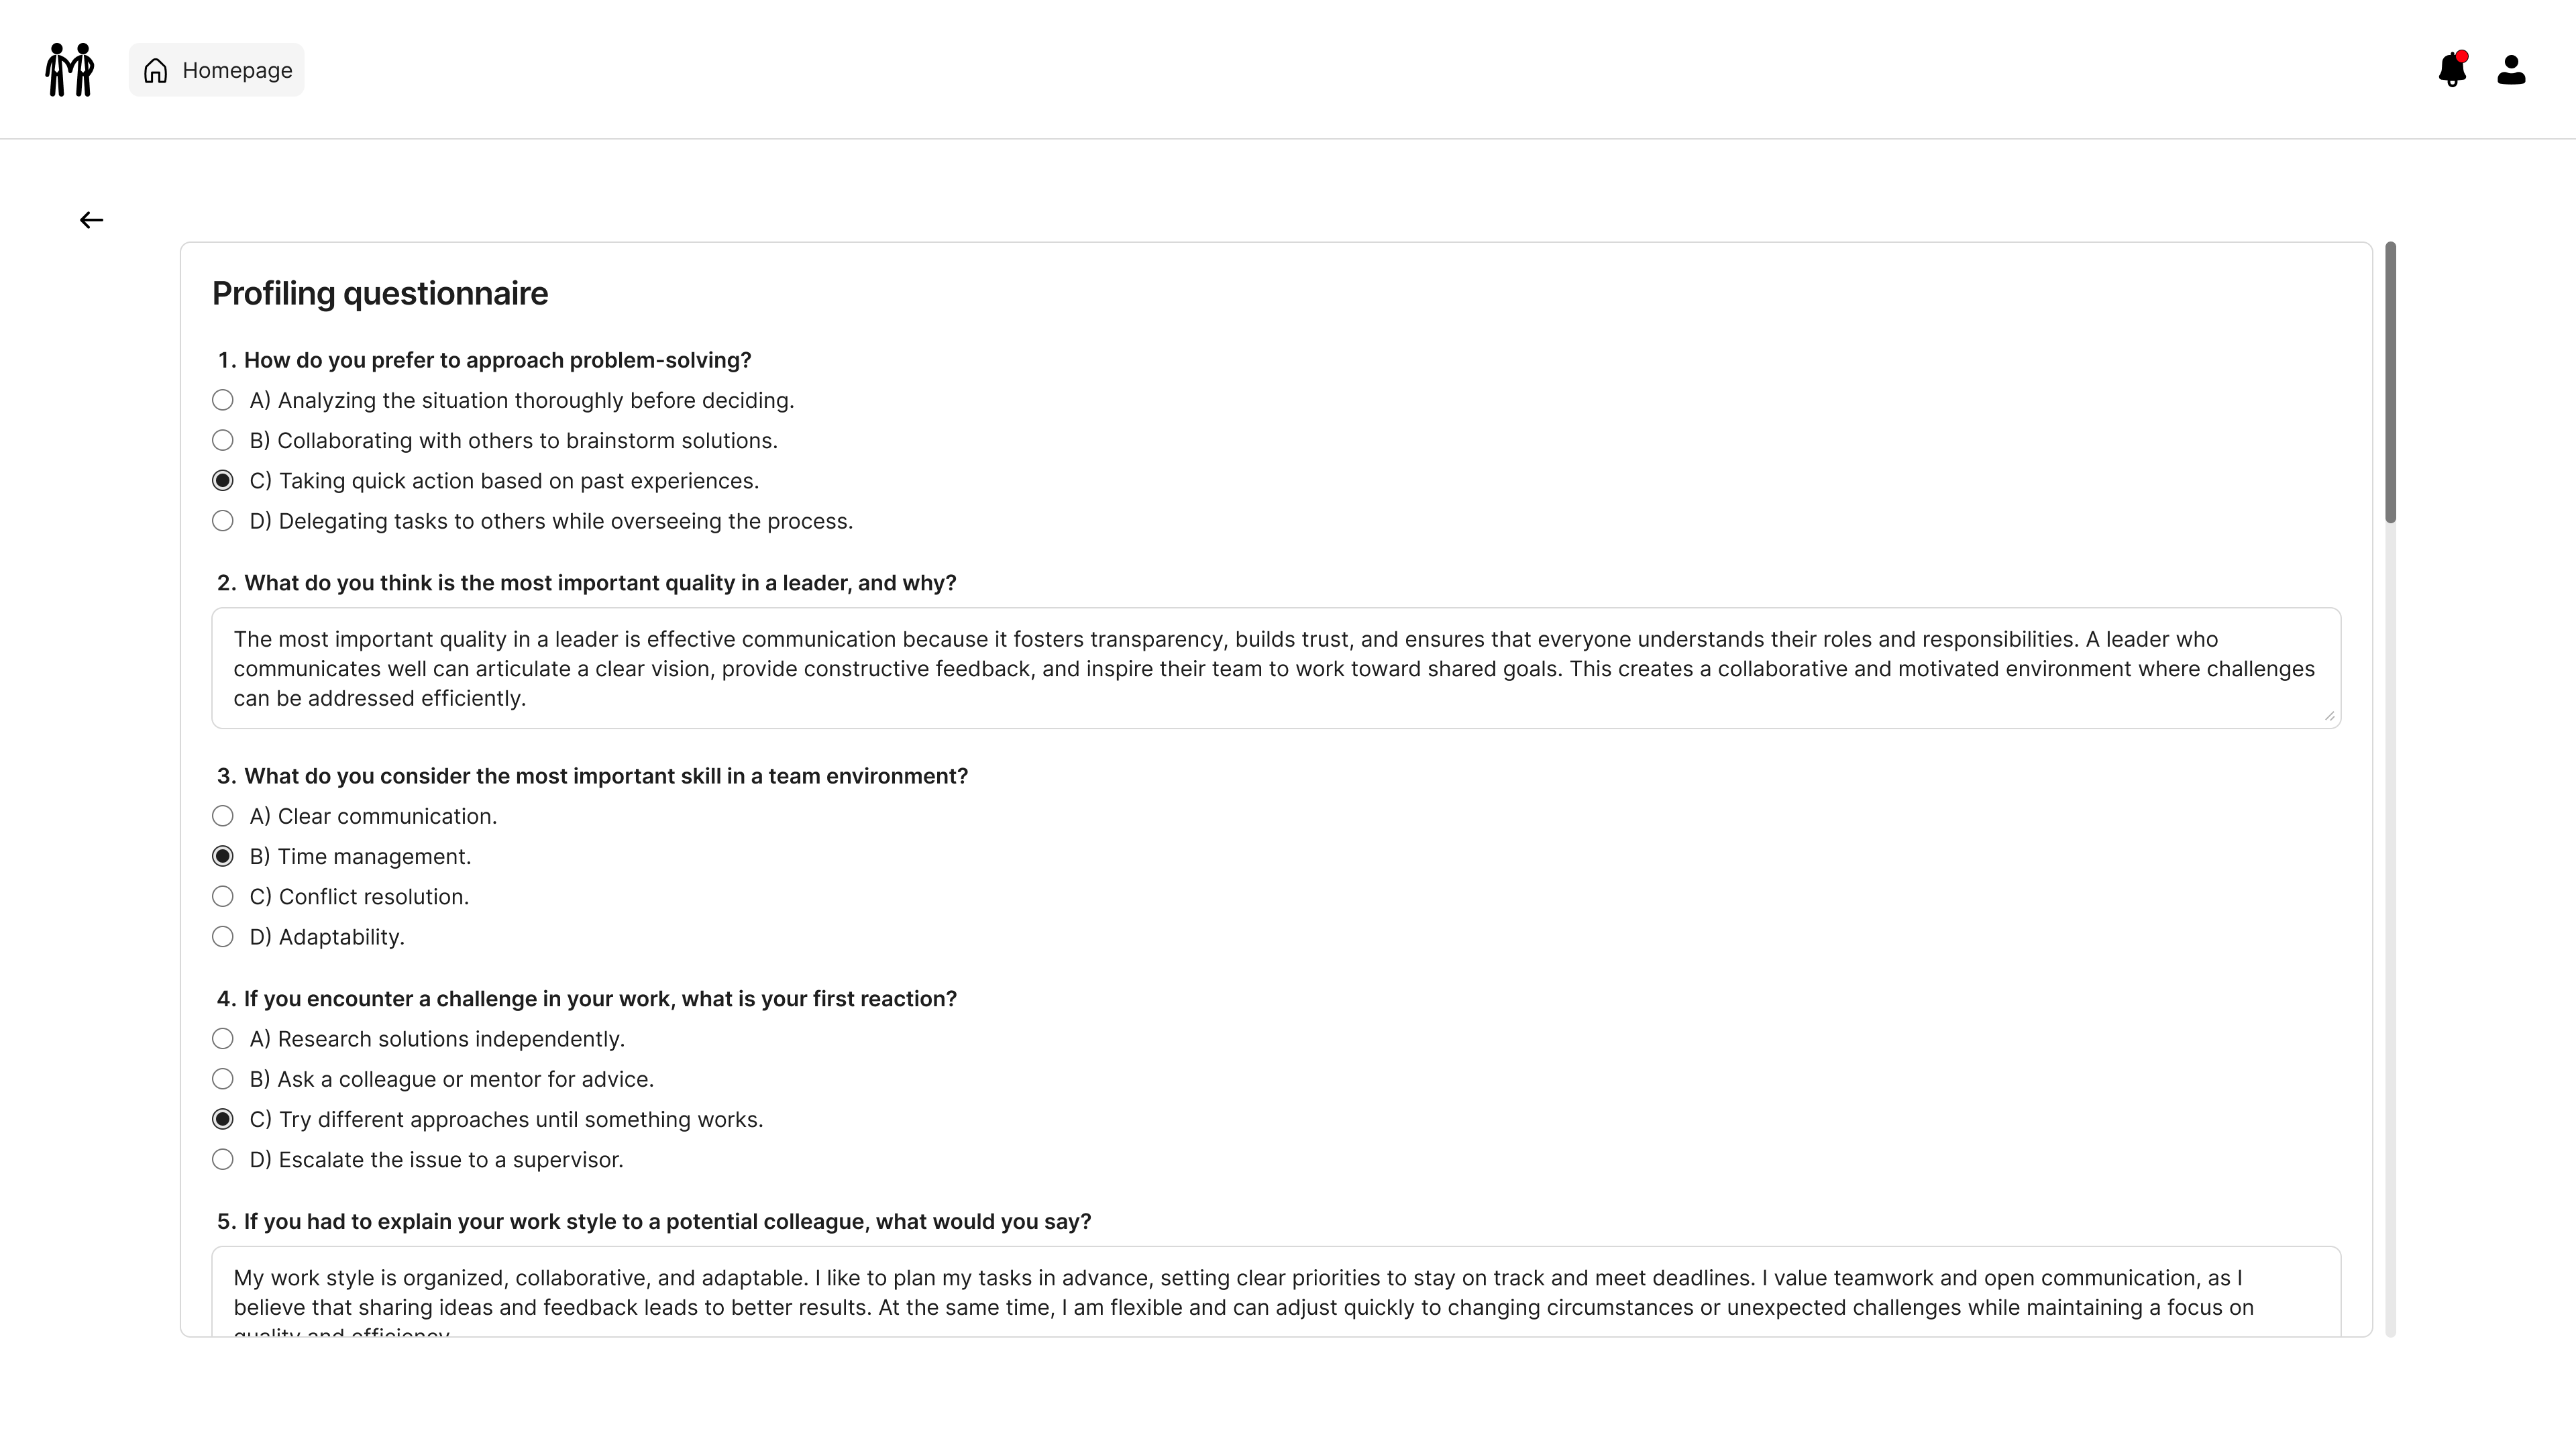
\includegraphics[width=1.0\textwidth]{Images/GUI/ST/Profiling Questionnaire - ST.png}}
    \caption{Profiling Questionnaire - ST}
    \label{fig:profiling-questionnaire-st}
\end{figure}

\par The Profiling Questionnaire page allows the ST to fill in a questionnaire to provide the company with more
information about themselves. The various questions will be automatically graded by the system to provide the
company with a synthetic evaluation of the ST. The questions will be provided manually by the CO.

\par A ST can only fill in the questionnaire only if they have been selected by the CO. This is de-facto the first
filtering step of the hiring process.

\subsection{Issue Reporting Form - ST}
\label{subsec:issue-reporting-form-st}%

\begin{figure}[H]
    \centering
    \fbox{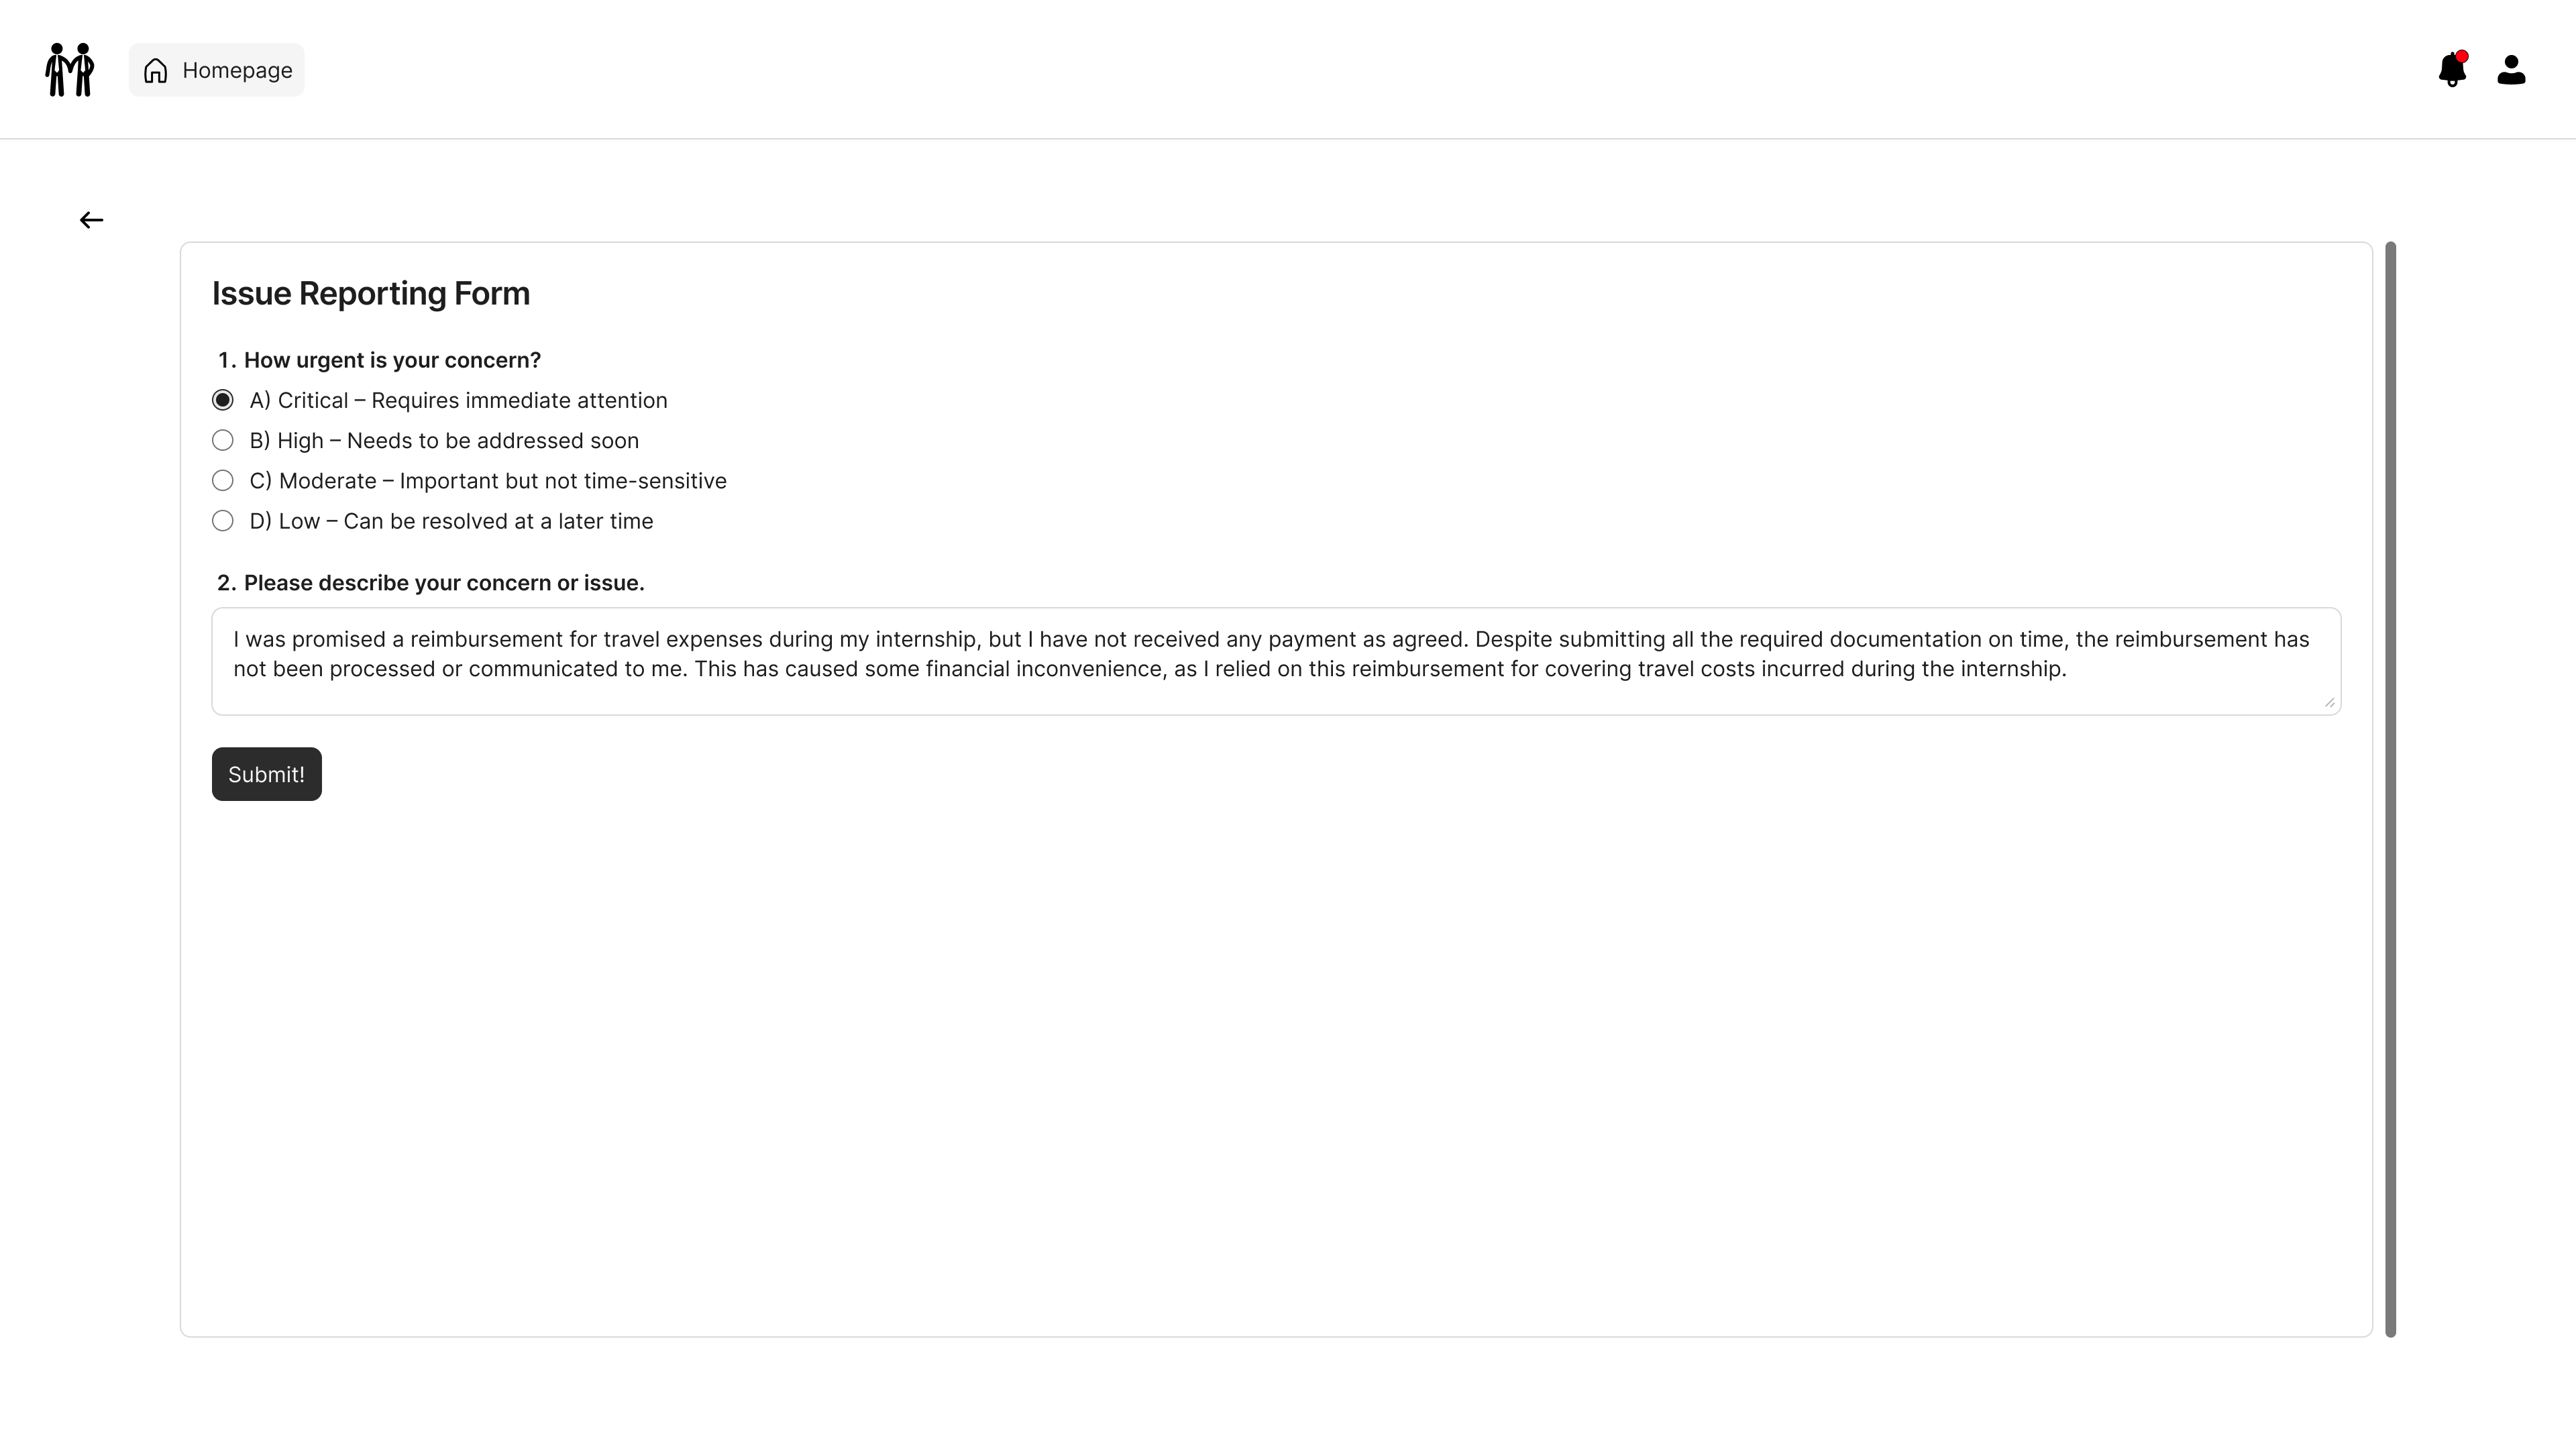
\includegraphics[width=1.0\textwidth]{Images/GUI/ST/Issue Reporting Form - ST.png}}
    \caption{Issue Reporting Form - ST}
    \label{fig:issue-reporting-form-st}
\end{figure}

\par The Issue Reporting Form page allows the ST to report any violations they have encountered during the
internship. The form is simple and allows the user to provide a description of the violation and any evidence they
have. The form is then sent to the company and the UN to evaluate the situation.

\par The user himself can choose the urgency of their issue.

\subsection{Internship Feedback Survey - ST}
\label{subsec:internship-feedback-survey-st}%

\begin{figure}[H]
    \centering
    \fbox{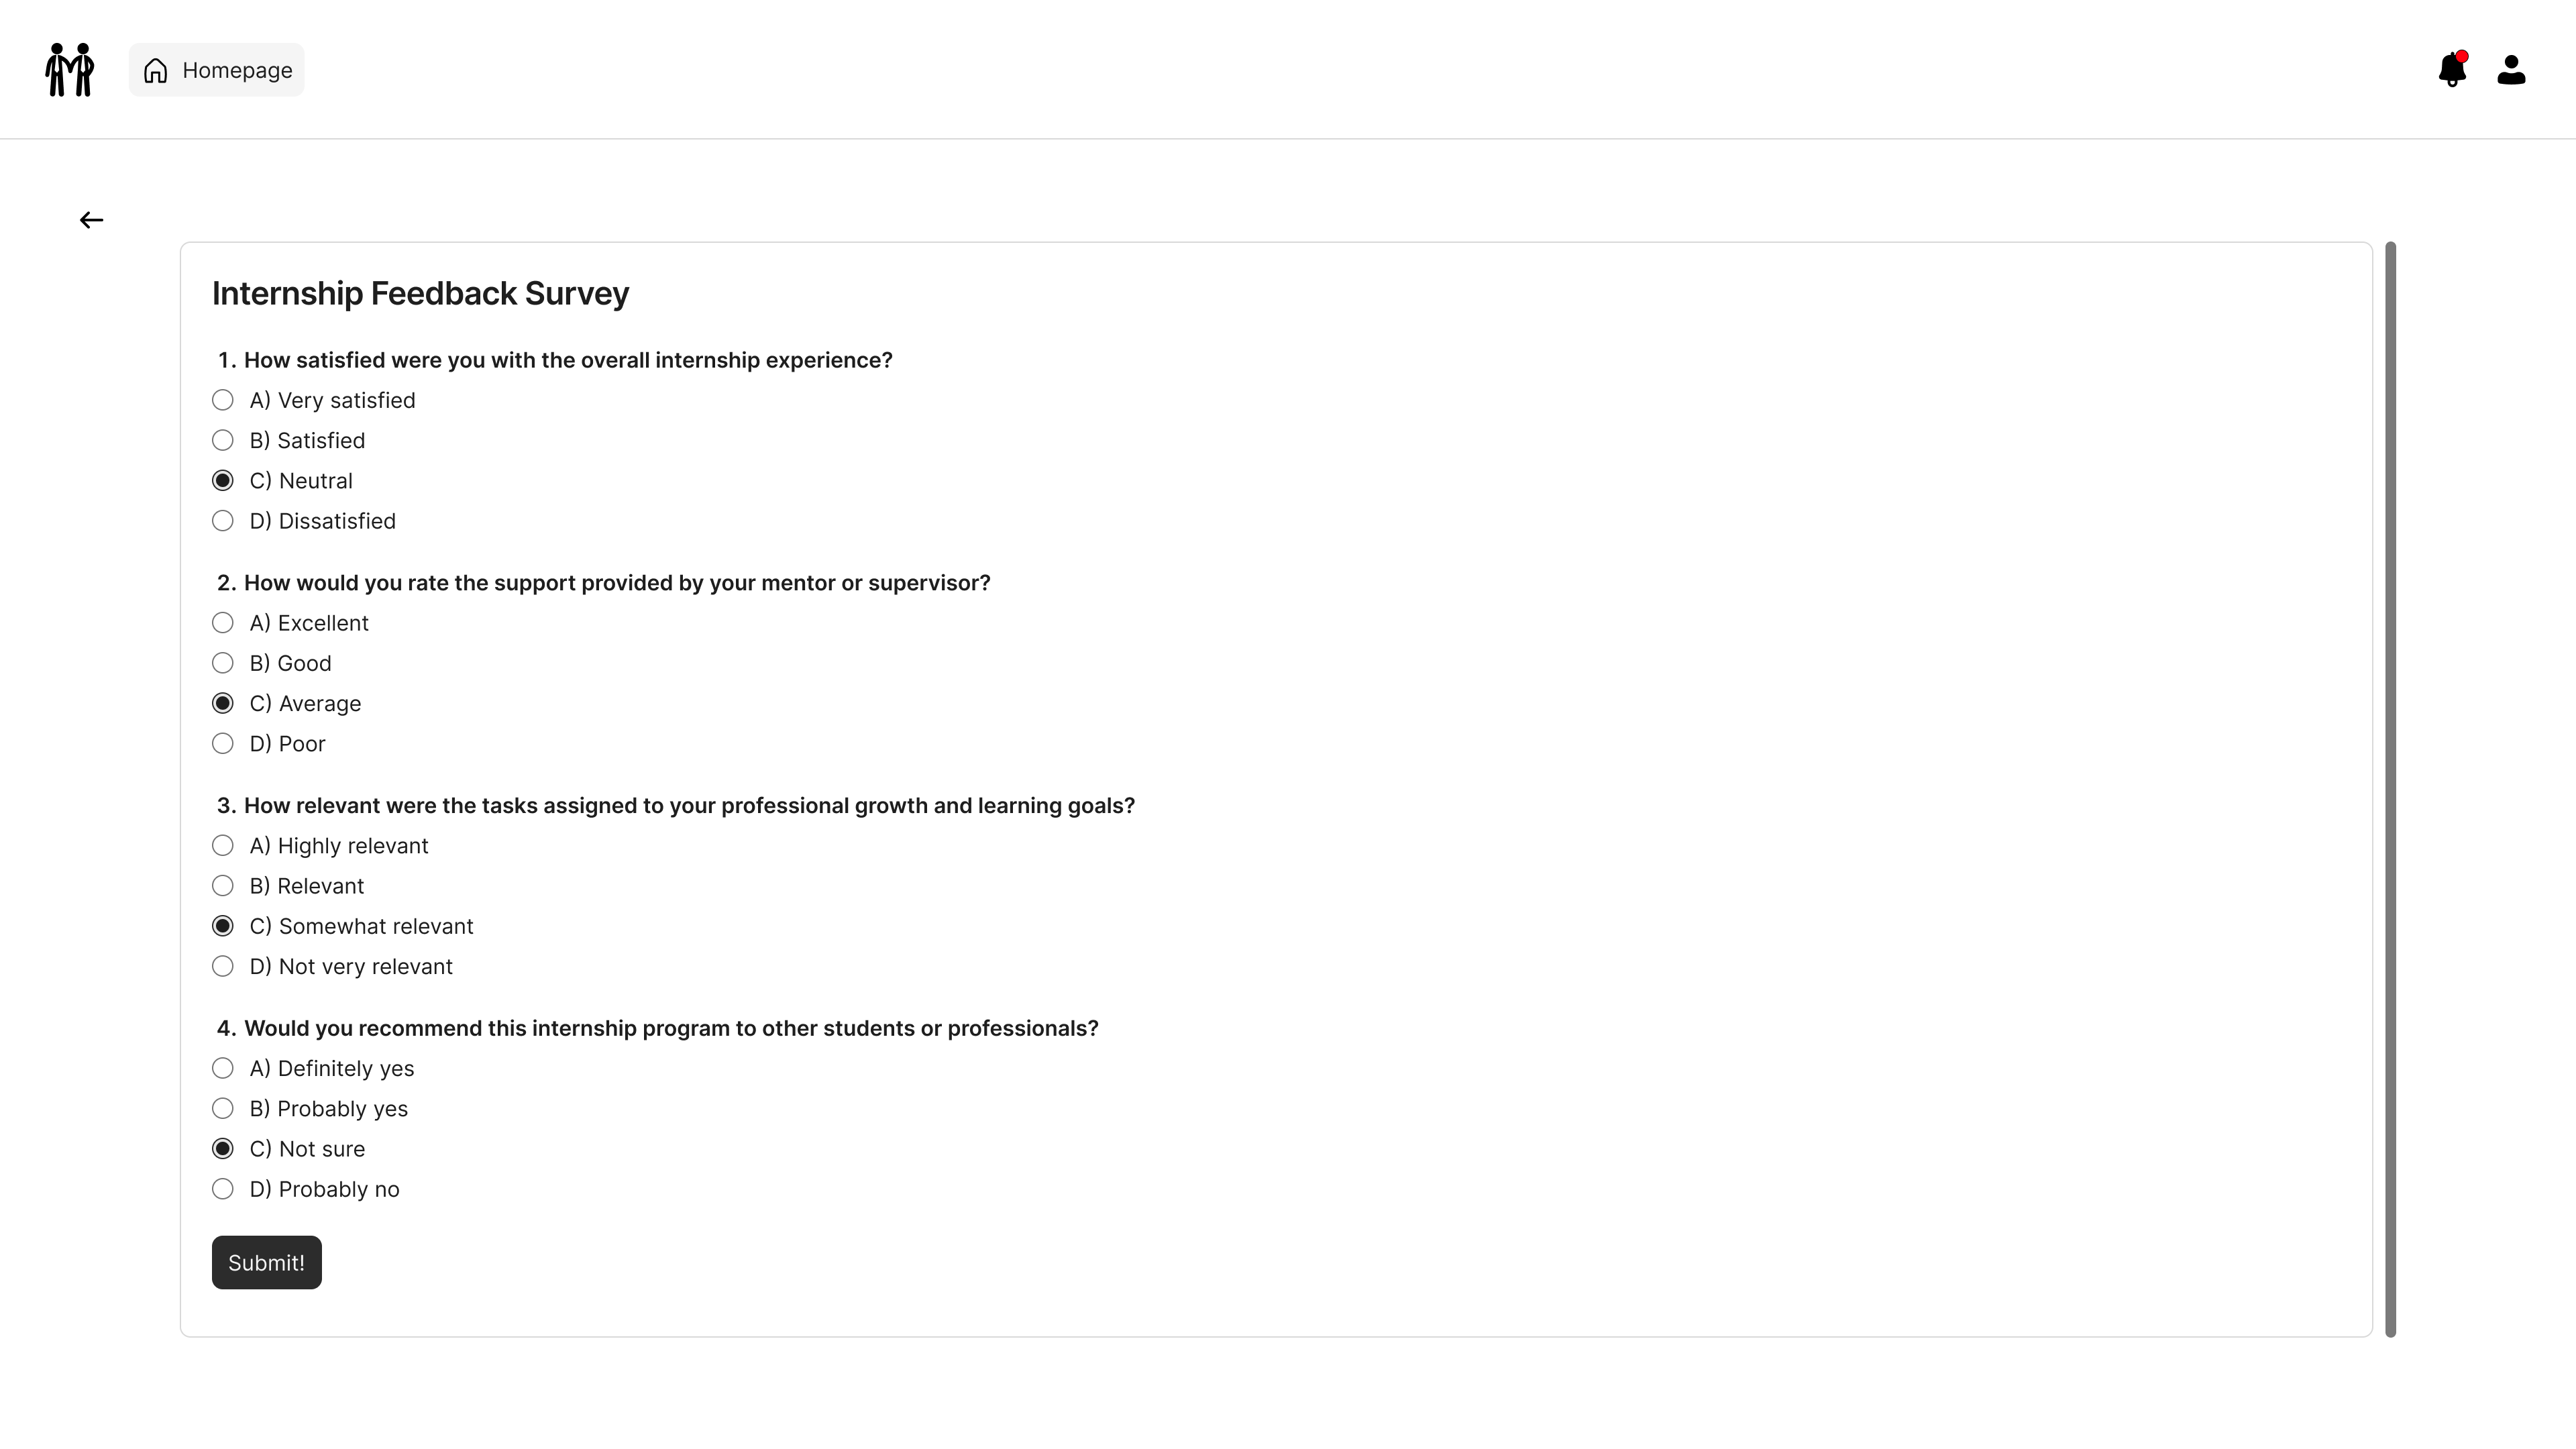
\includegraphics[width=1.0\textwidth]{Images/GUI/ST/Internship Feedback Survey - ST.png}}
    \caption{Internship Feedback Survey - ST}
    \label{fig:internship-feedback-survey-st}
\end{figure}

\par The Internship Feedback Survey page allows the ST to provide a final evaluation on the internship. S\&C and UN
will use this information to improve the quality of the internships and the platform.

\section{User Flow: CO}
\label{sec:user-flow-co}%

\begin{figure}[H]
    \centering
    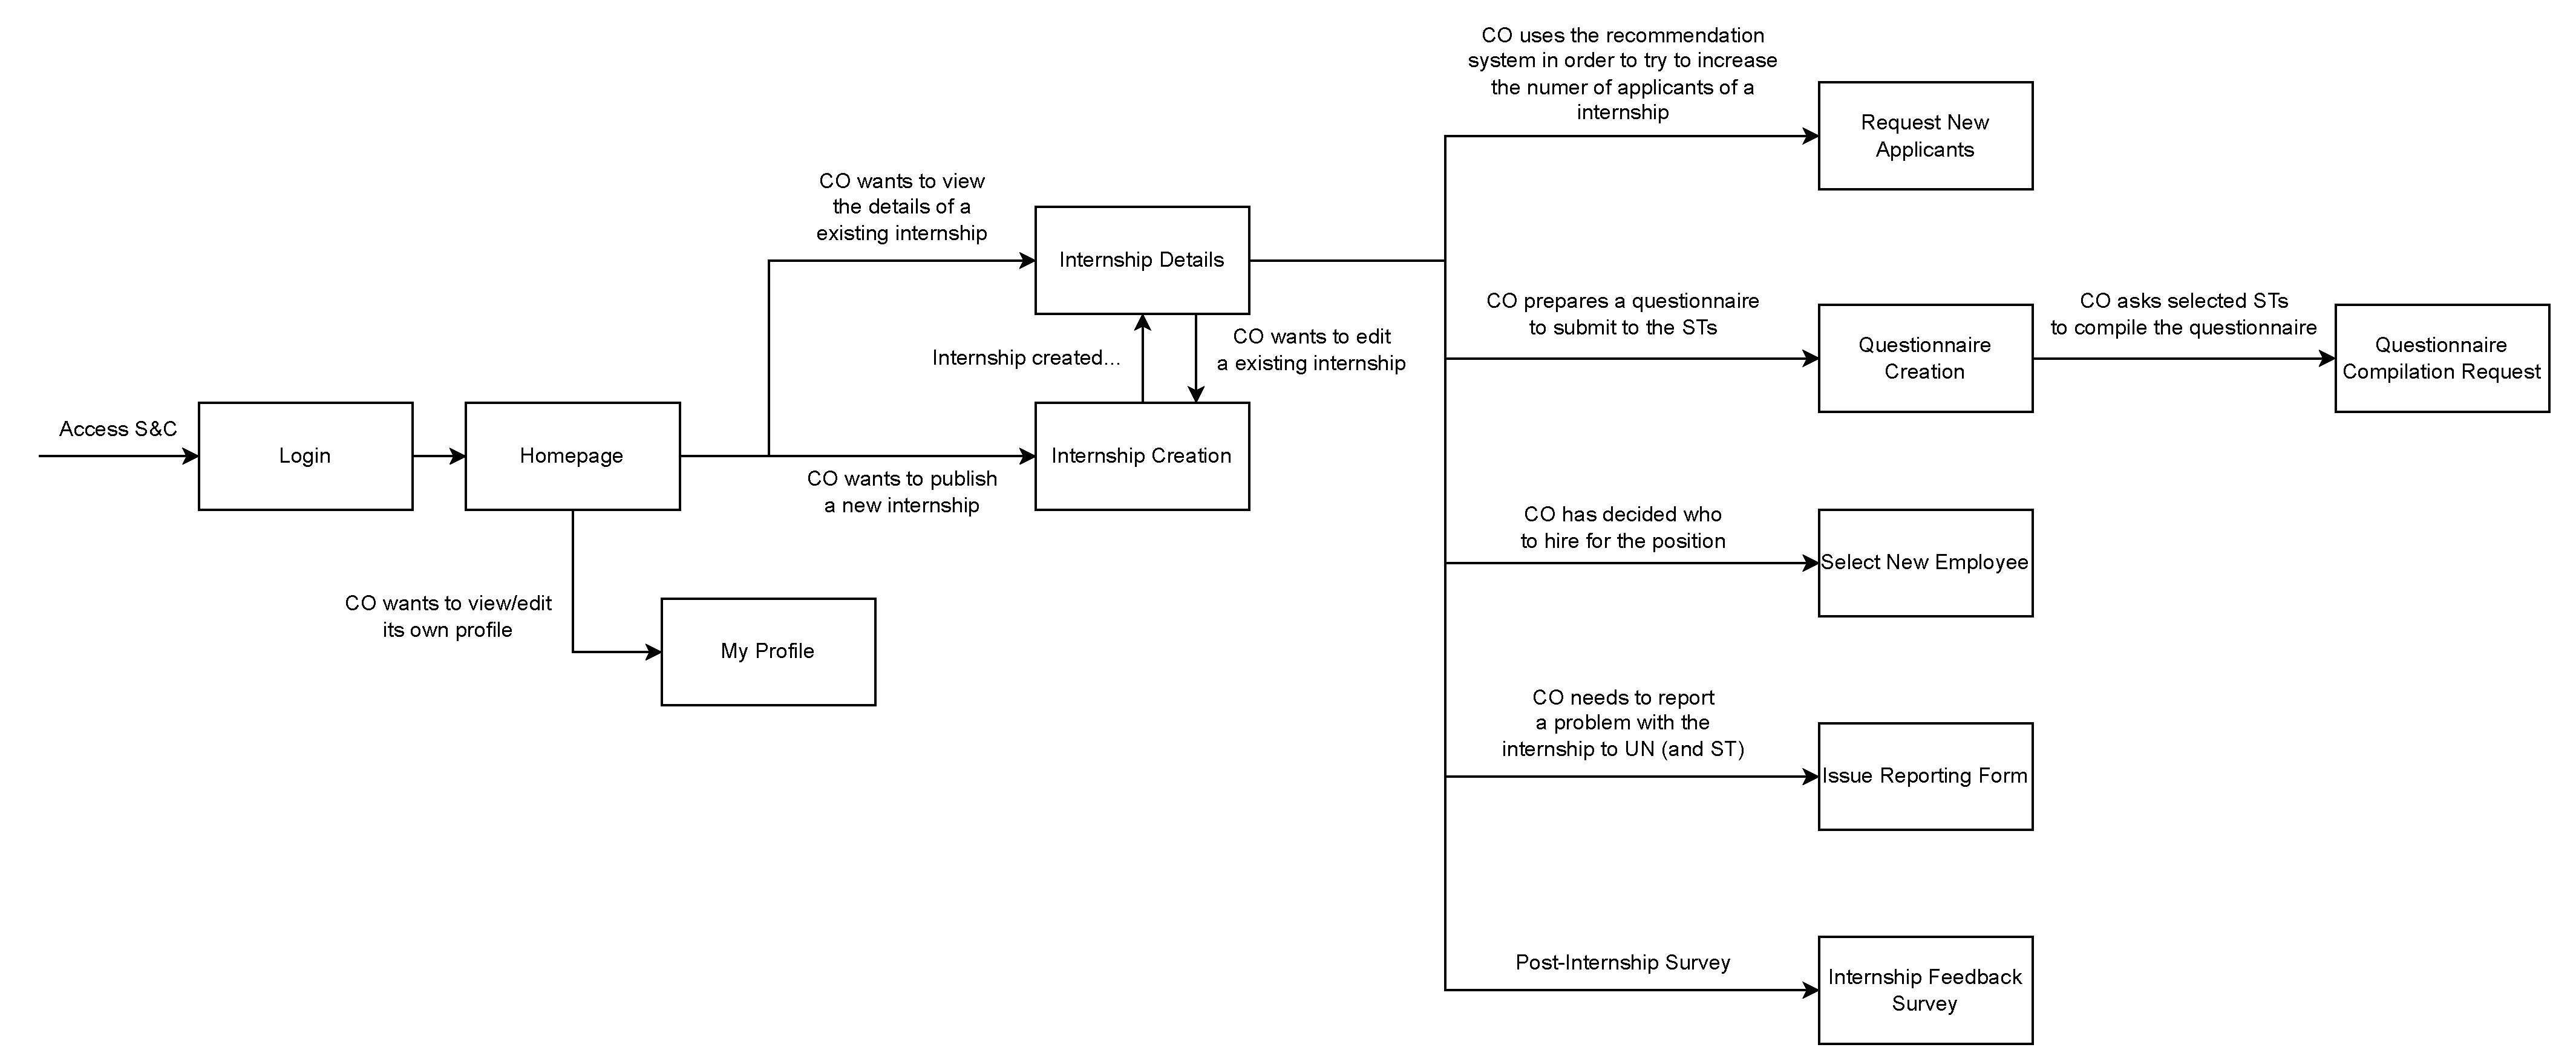
\includegraphics[width=1.0\textwidth]{Images/GUI/CO/Diagram.pdf}
    \caption{CO User Flow Diagram}
    \label{fig:co-user-flow-diagram}
\end{figure}

\par Now is presented the user flow diagram for the CO. The CO uses the Login page to authenticate and access S\&C
using plain credentials provided by S\&C's administrators. Once logged in, the CO is redirected to the Homepage, here
the user can view all the internships they have posted (past and present) and view their details (Internship Details).
The Login page is the same for all the users and as such will not be presented again.

\par On the Internship Details page, the CO can view all the details of the internship, edit them - up until the
application deadline - and send notifications to the STs that the system has deemed as a good match for the internship
(more details will be provided later). After the application deadline, the CO can create the questionnaire
(Questionnaire Creation) to submit to the STs that the CO has selected - thus creating a first filter - using the
Questionnaire Compilation Request. Using the Select New Employee page the CO can view the results of said
questionnaire and select the ST that will be hired. Once the internship is over, the CO can access the Internship
Feedback Survey page to evaluate the internship. In case of issues, the CO can access the Issue Reporting Form page
to report them.

\par The creation of a new internship is done using the Internship Creation page also accessible from the Homepage: the
CO will be presented with a two-step form to fill in all the required information. Finally, the CO can access and
update their profile using the Profile page accessible from a button in the header.

\subsection{Homepage - CO}
\label{subsec:homepage-co}%

\begin{figure}[H]
    \centering
    \fbox{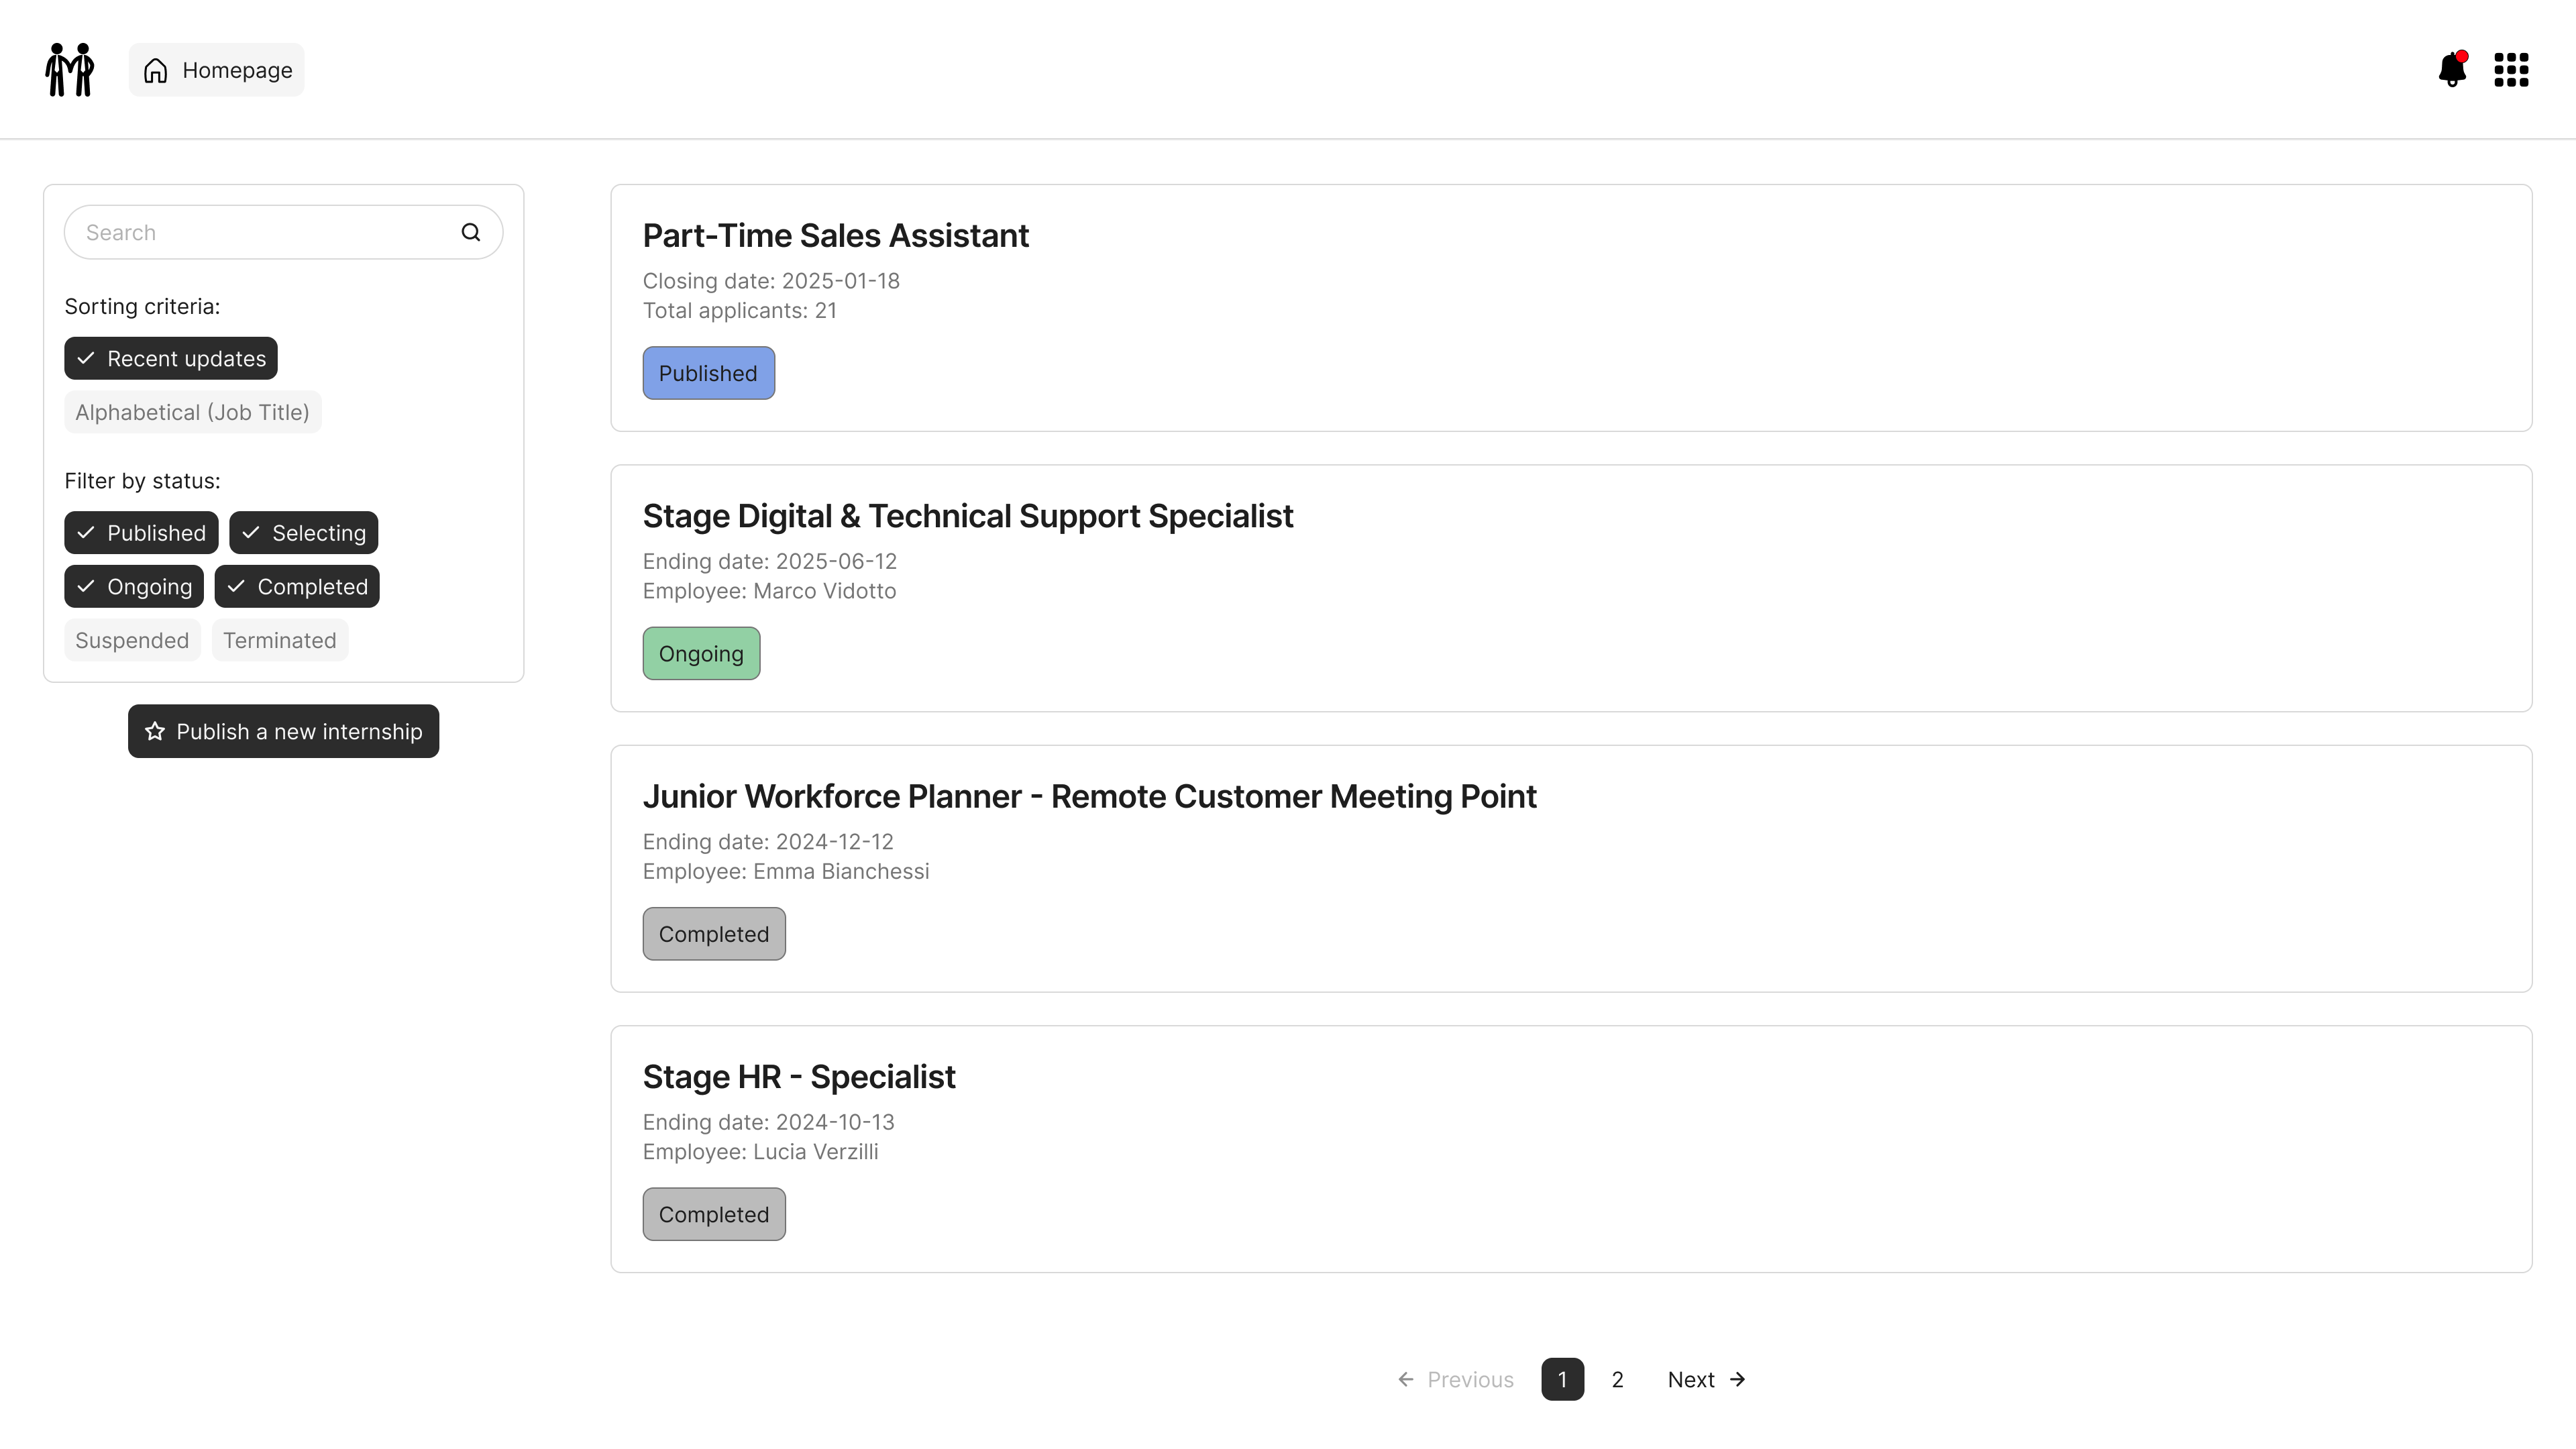
\includegraphics[width=1.0\textwidth]{Images/GUI/CO/Homepage - CO.png}}
    \caption{Homepage - CO}
    \label{fig:homepage-co}
\end{figure}

\par The Homepage is the main page for the CO. Here the user can view all the internships they have posted (past and
present) and view their details. Proper filters are provided to allow the user to search for internships based on
their preferences and needs. Also, in this page is present a button that allows the CO to create a new internship.

\par As all the other pages, the header is present and allows the user to: access their profile, log out from the
platform and view any new notifications from the related submenu.

\begin{figure}[H]
    \centering
    \fbox{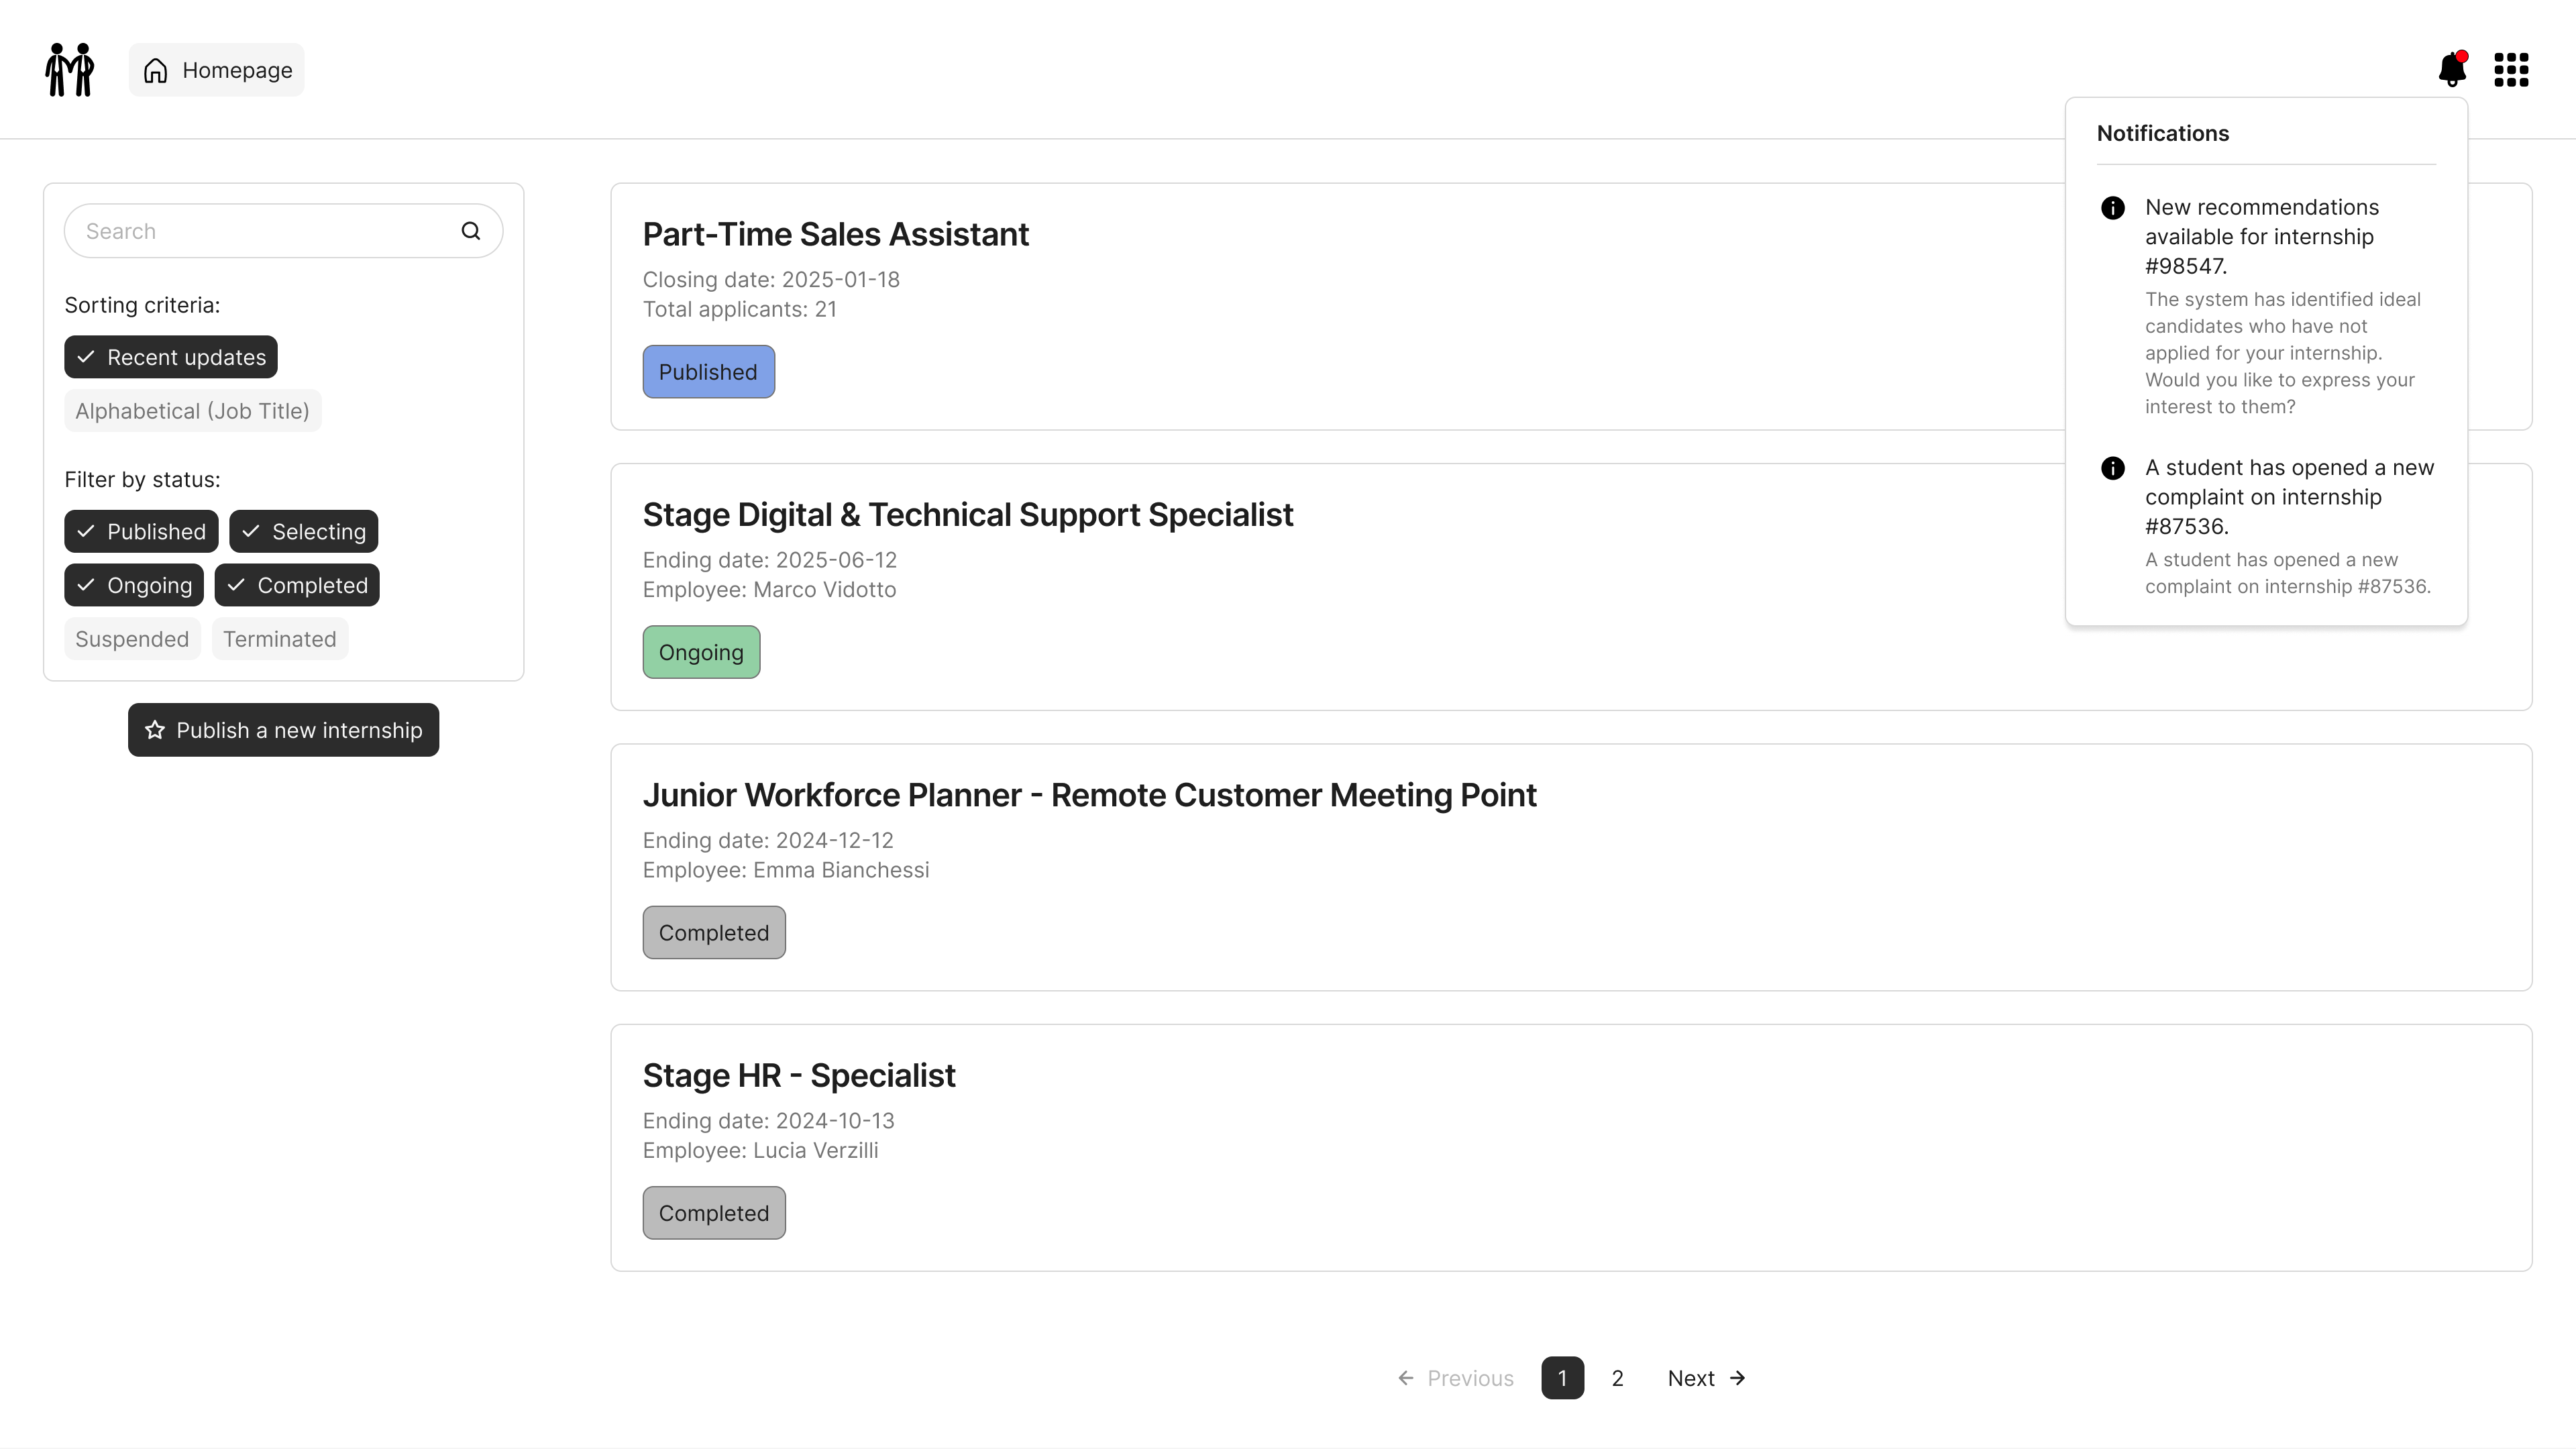
\includegraphics[width=1.0\textwidth]{Images/GUI/CO/Homepage - CO - Notification.png}}
    \caption{Homepage - CO - Notification}
    \label{fig:homepage-co-notification}
\end{figure}

\begin{figure}[H]
    \centering
    \fbox{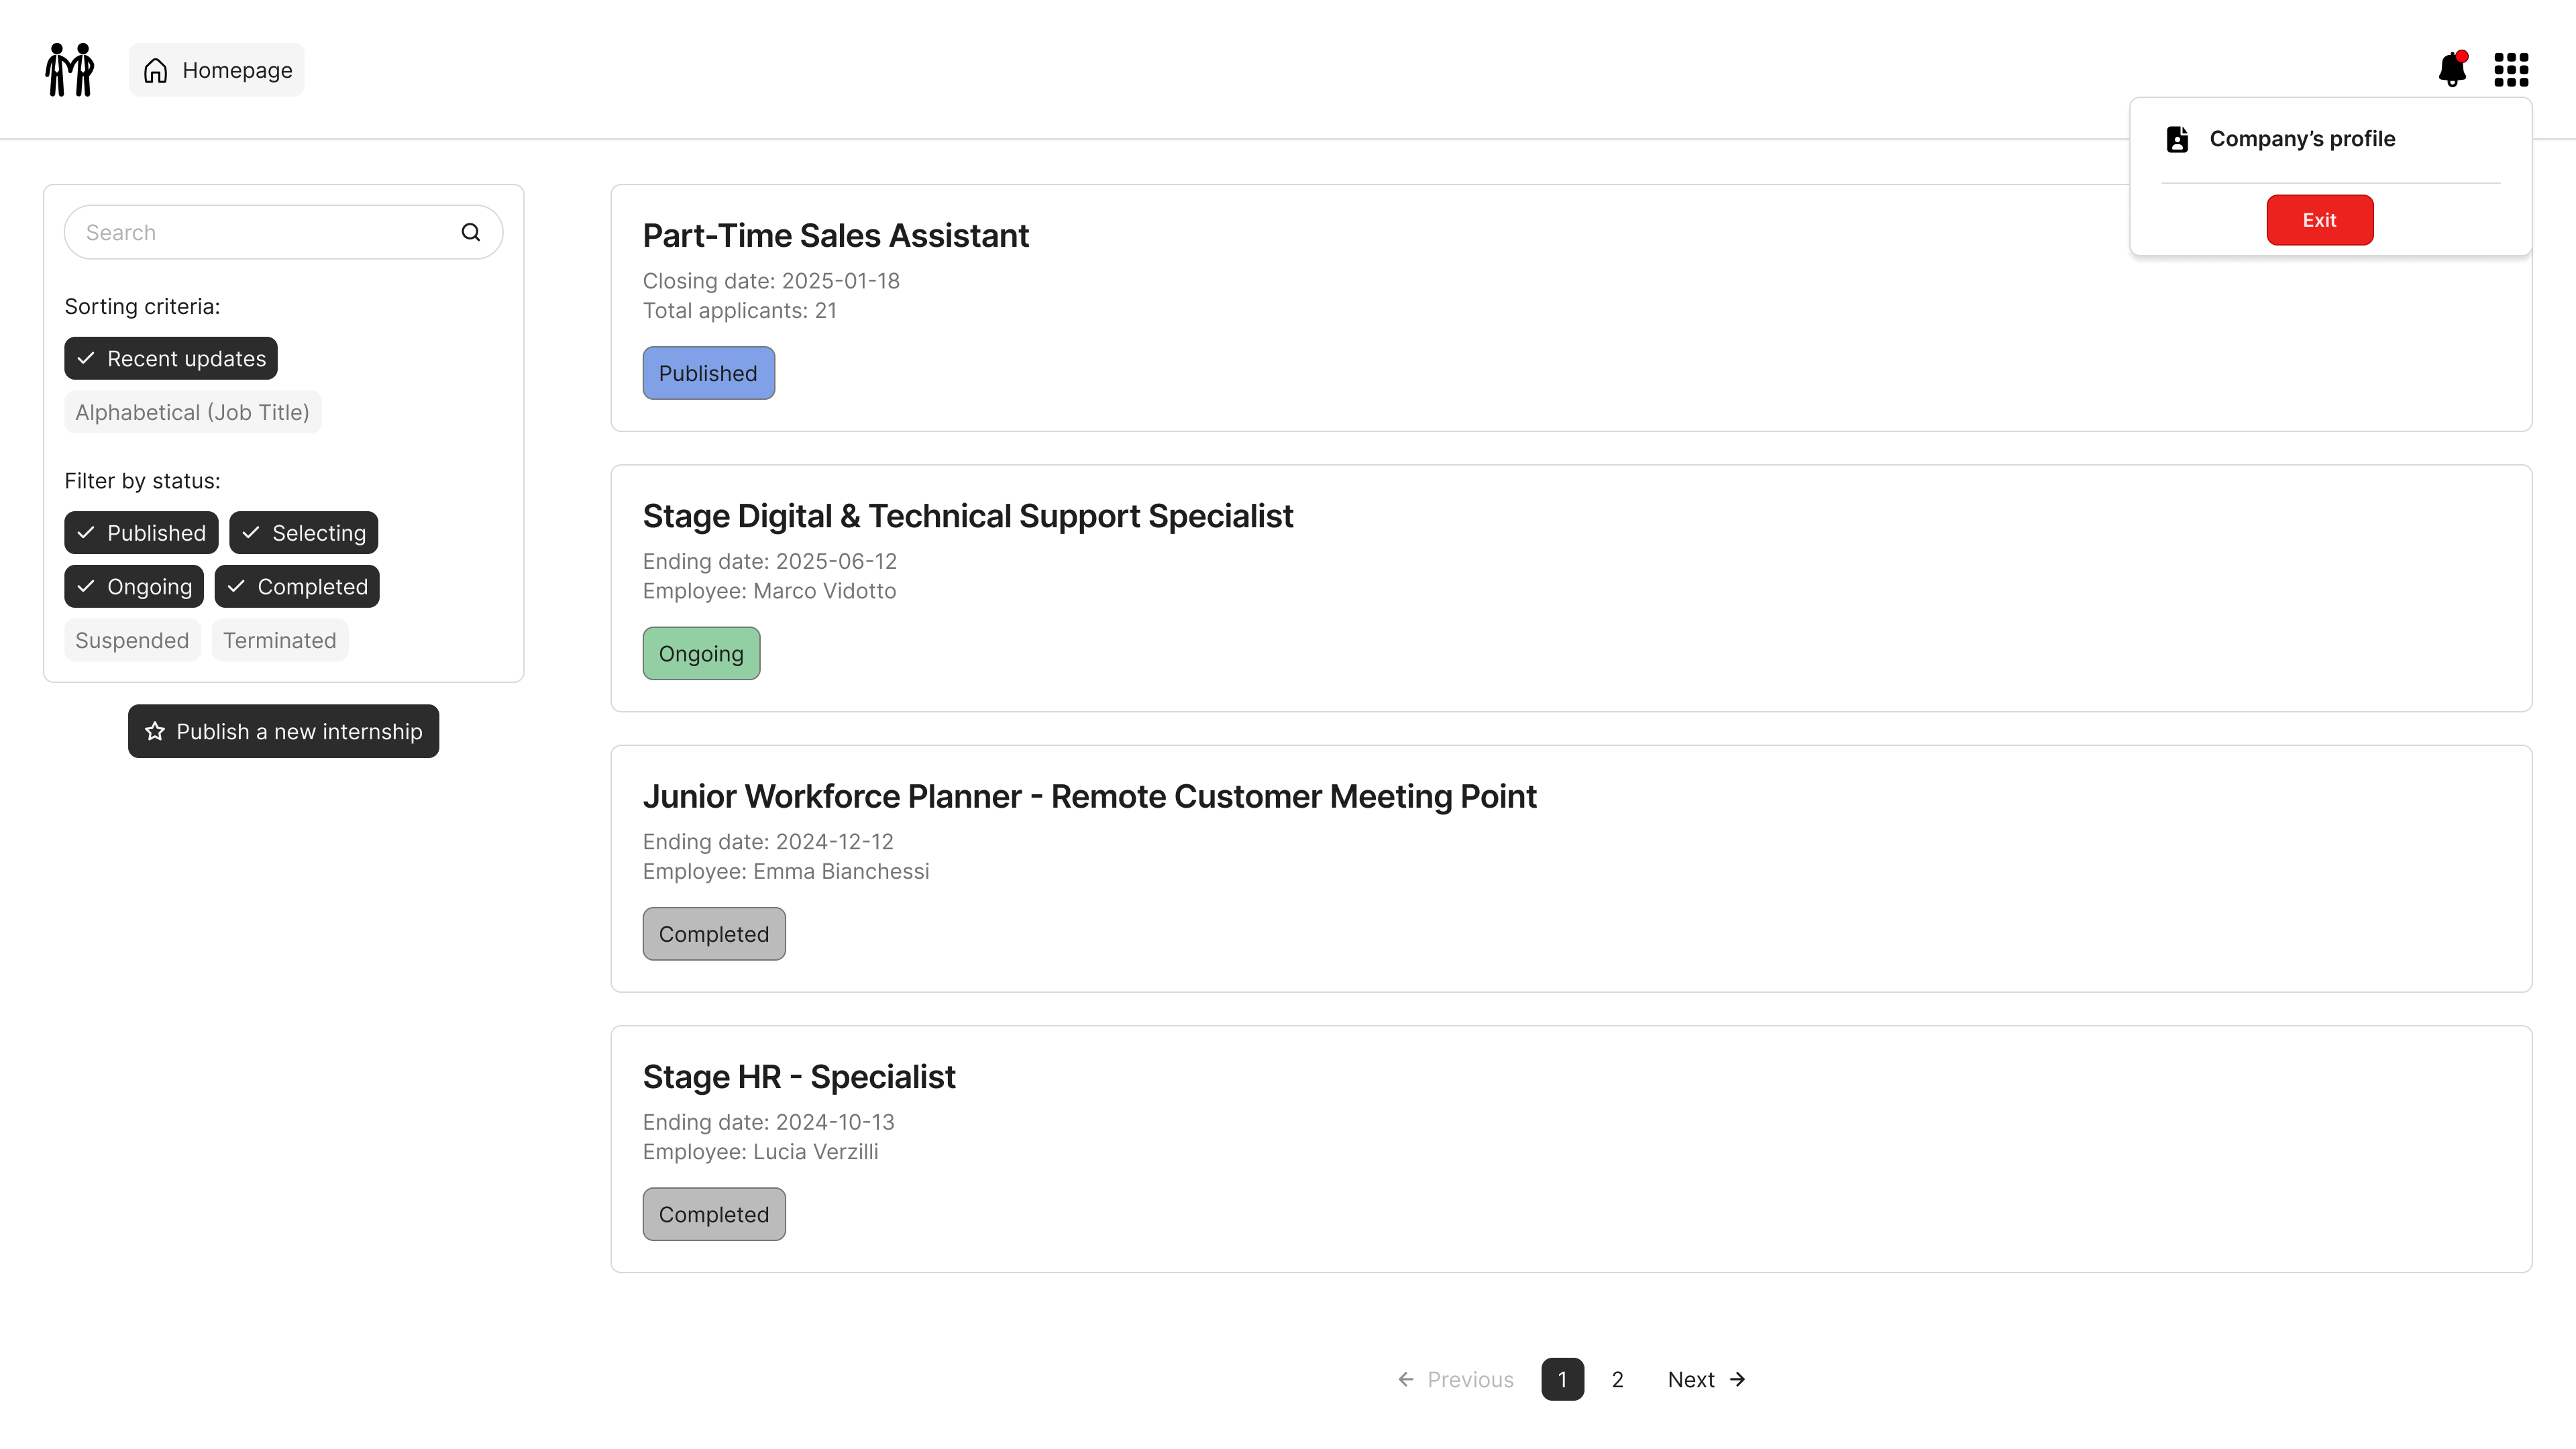
\includegraphics[width=1.0\textwidth]{Images/GUI/CO/Homepage - CO - Profile.png}}
    \caption{Homepage - CO - Profile}
    \label{fig:homepage-co-profile}
\end{figure}

\subsection{Internship Creation - CO}
\label{subsec:internship-creation-co}%

\begin{figure}[H]
    \centering
    \fbox{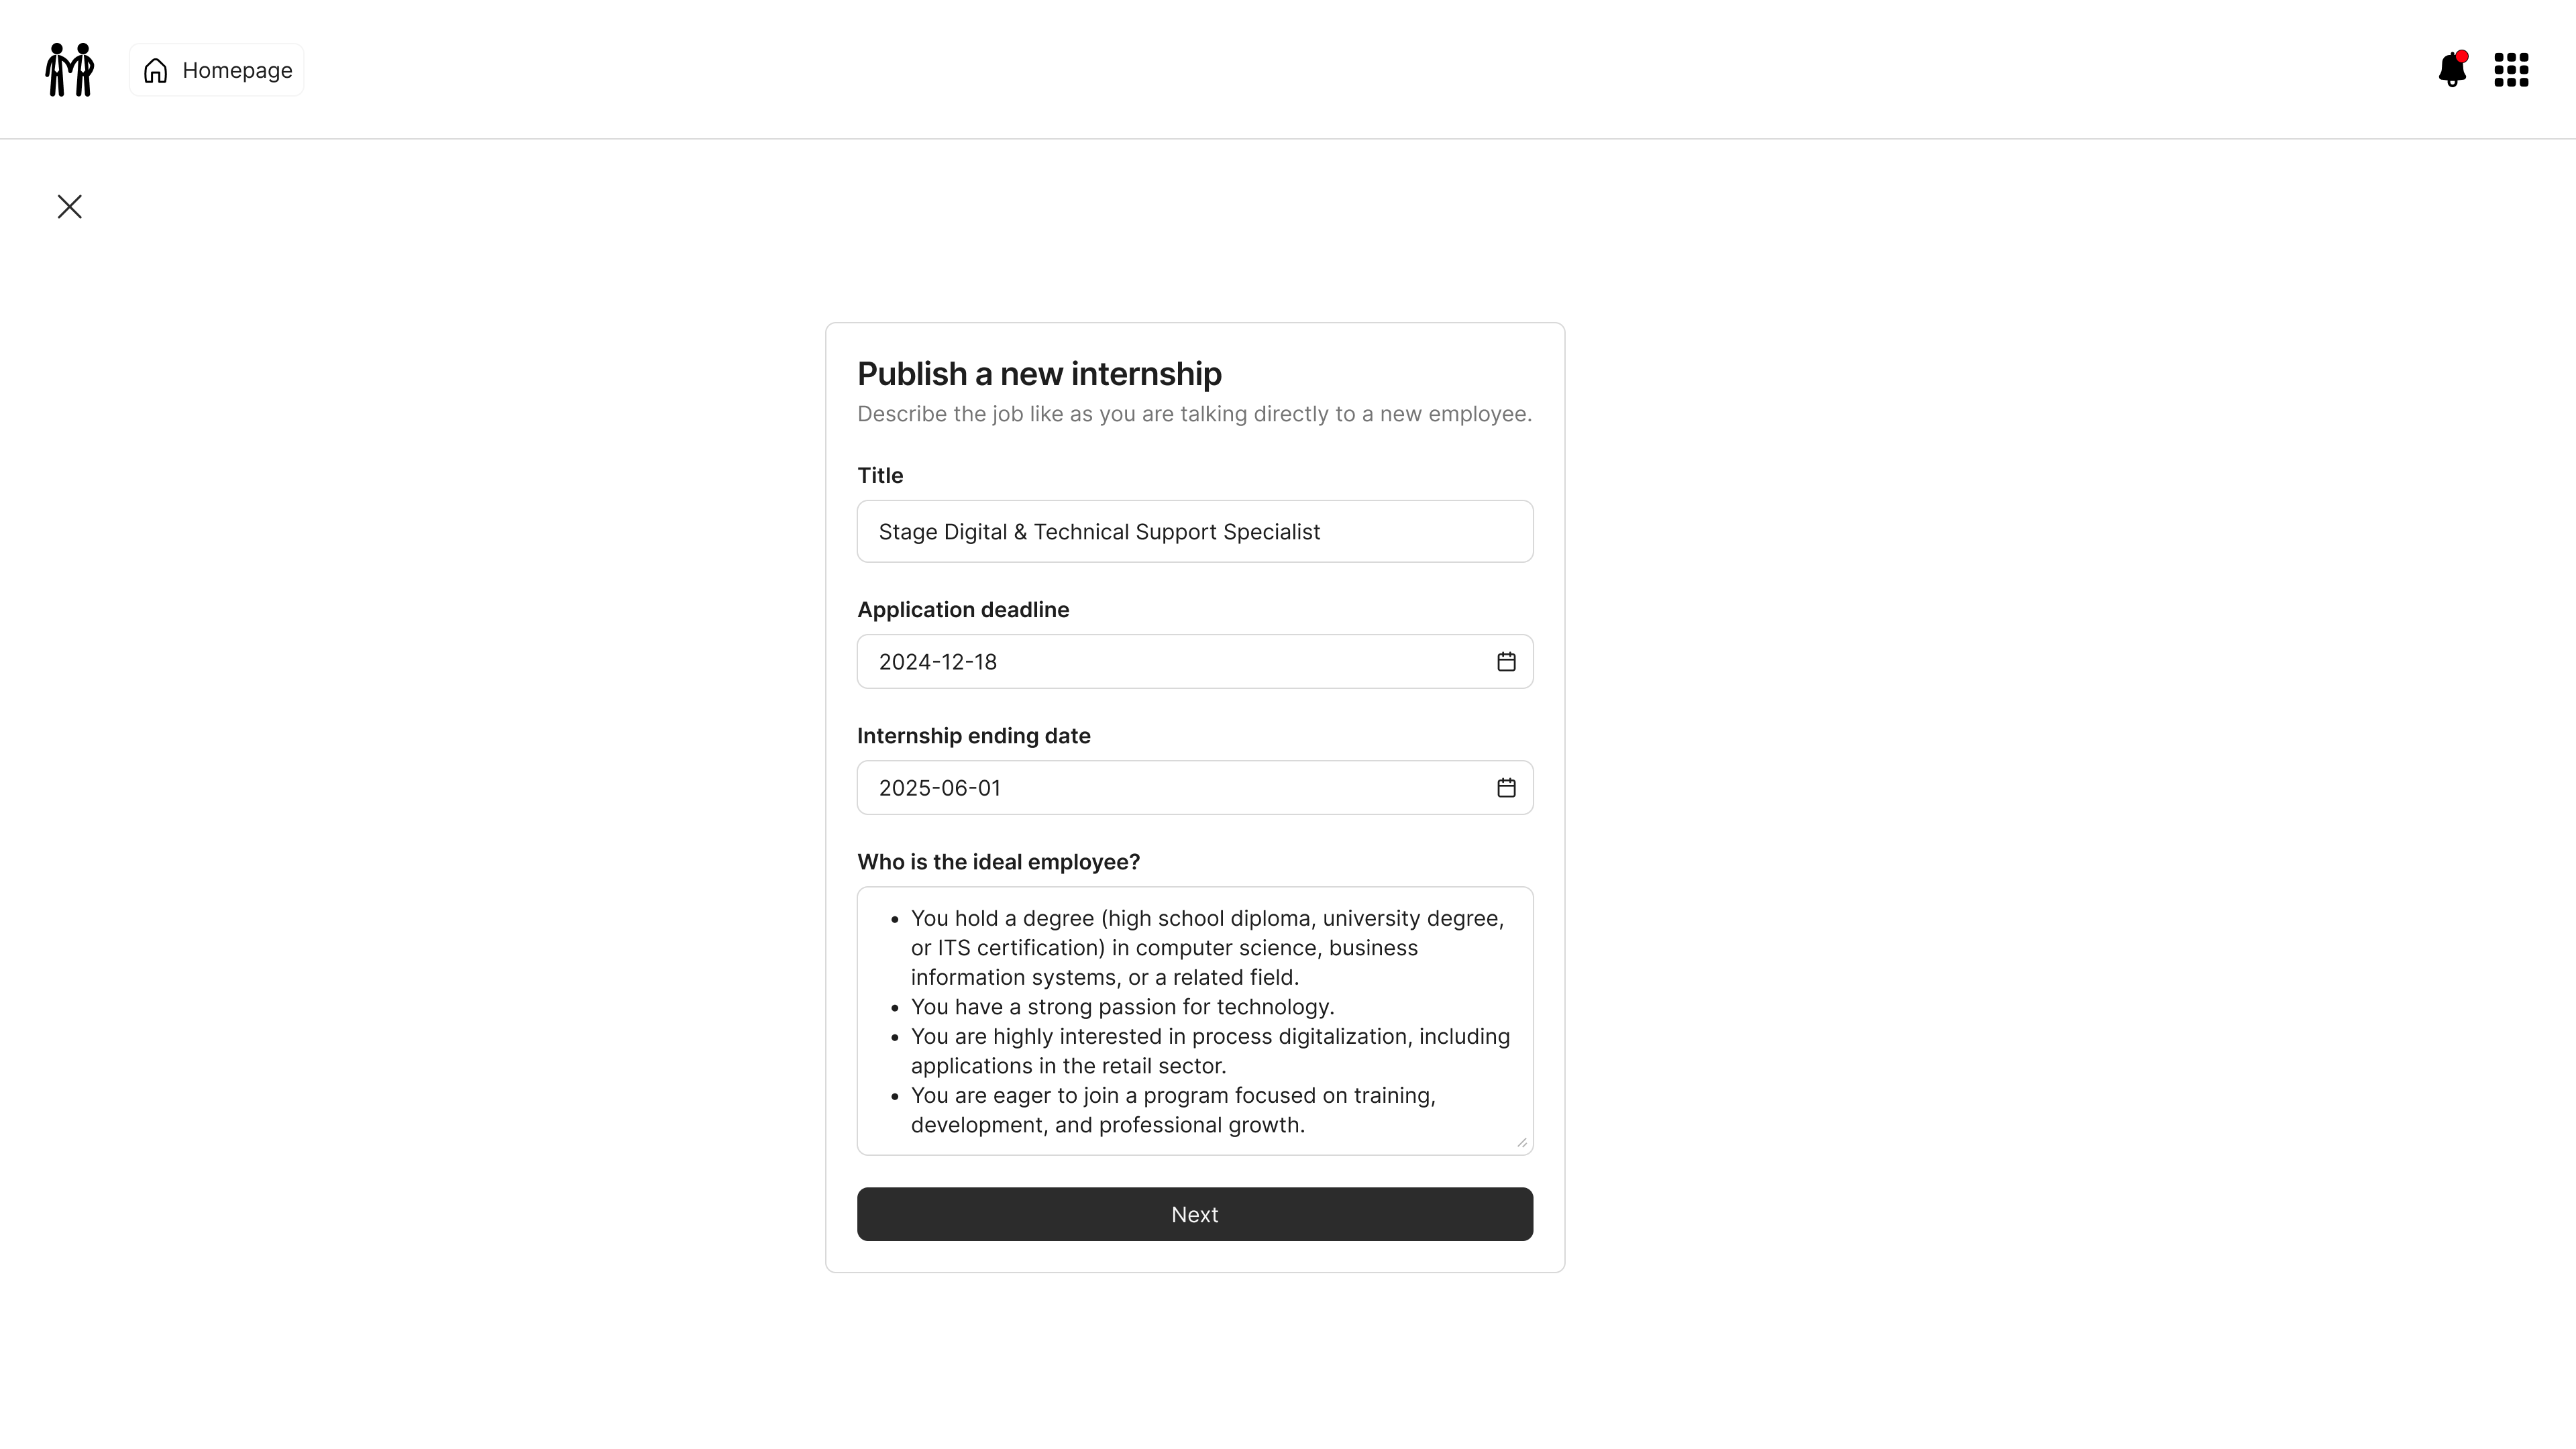
\includegraphics[width=1.0\textwidth]{Images/GUI/CO/Internship Creation - 1 - CO.png}}
    \caption{Internship Creation - 1 - CO}
    \label{fig:internship-creation-1-co}
\end{figure}

\begin{figure}[H]
    \centering
    \fbox{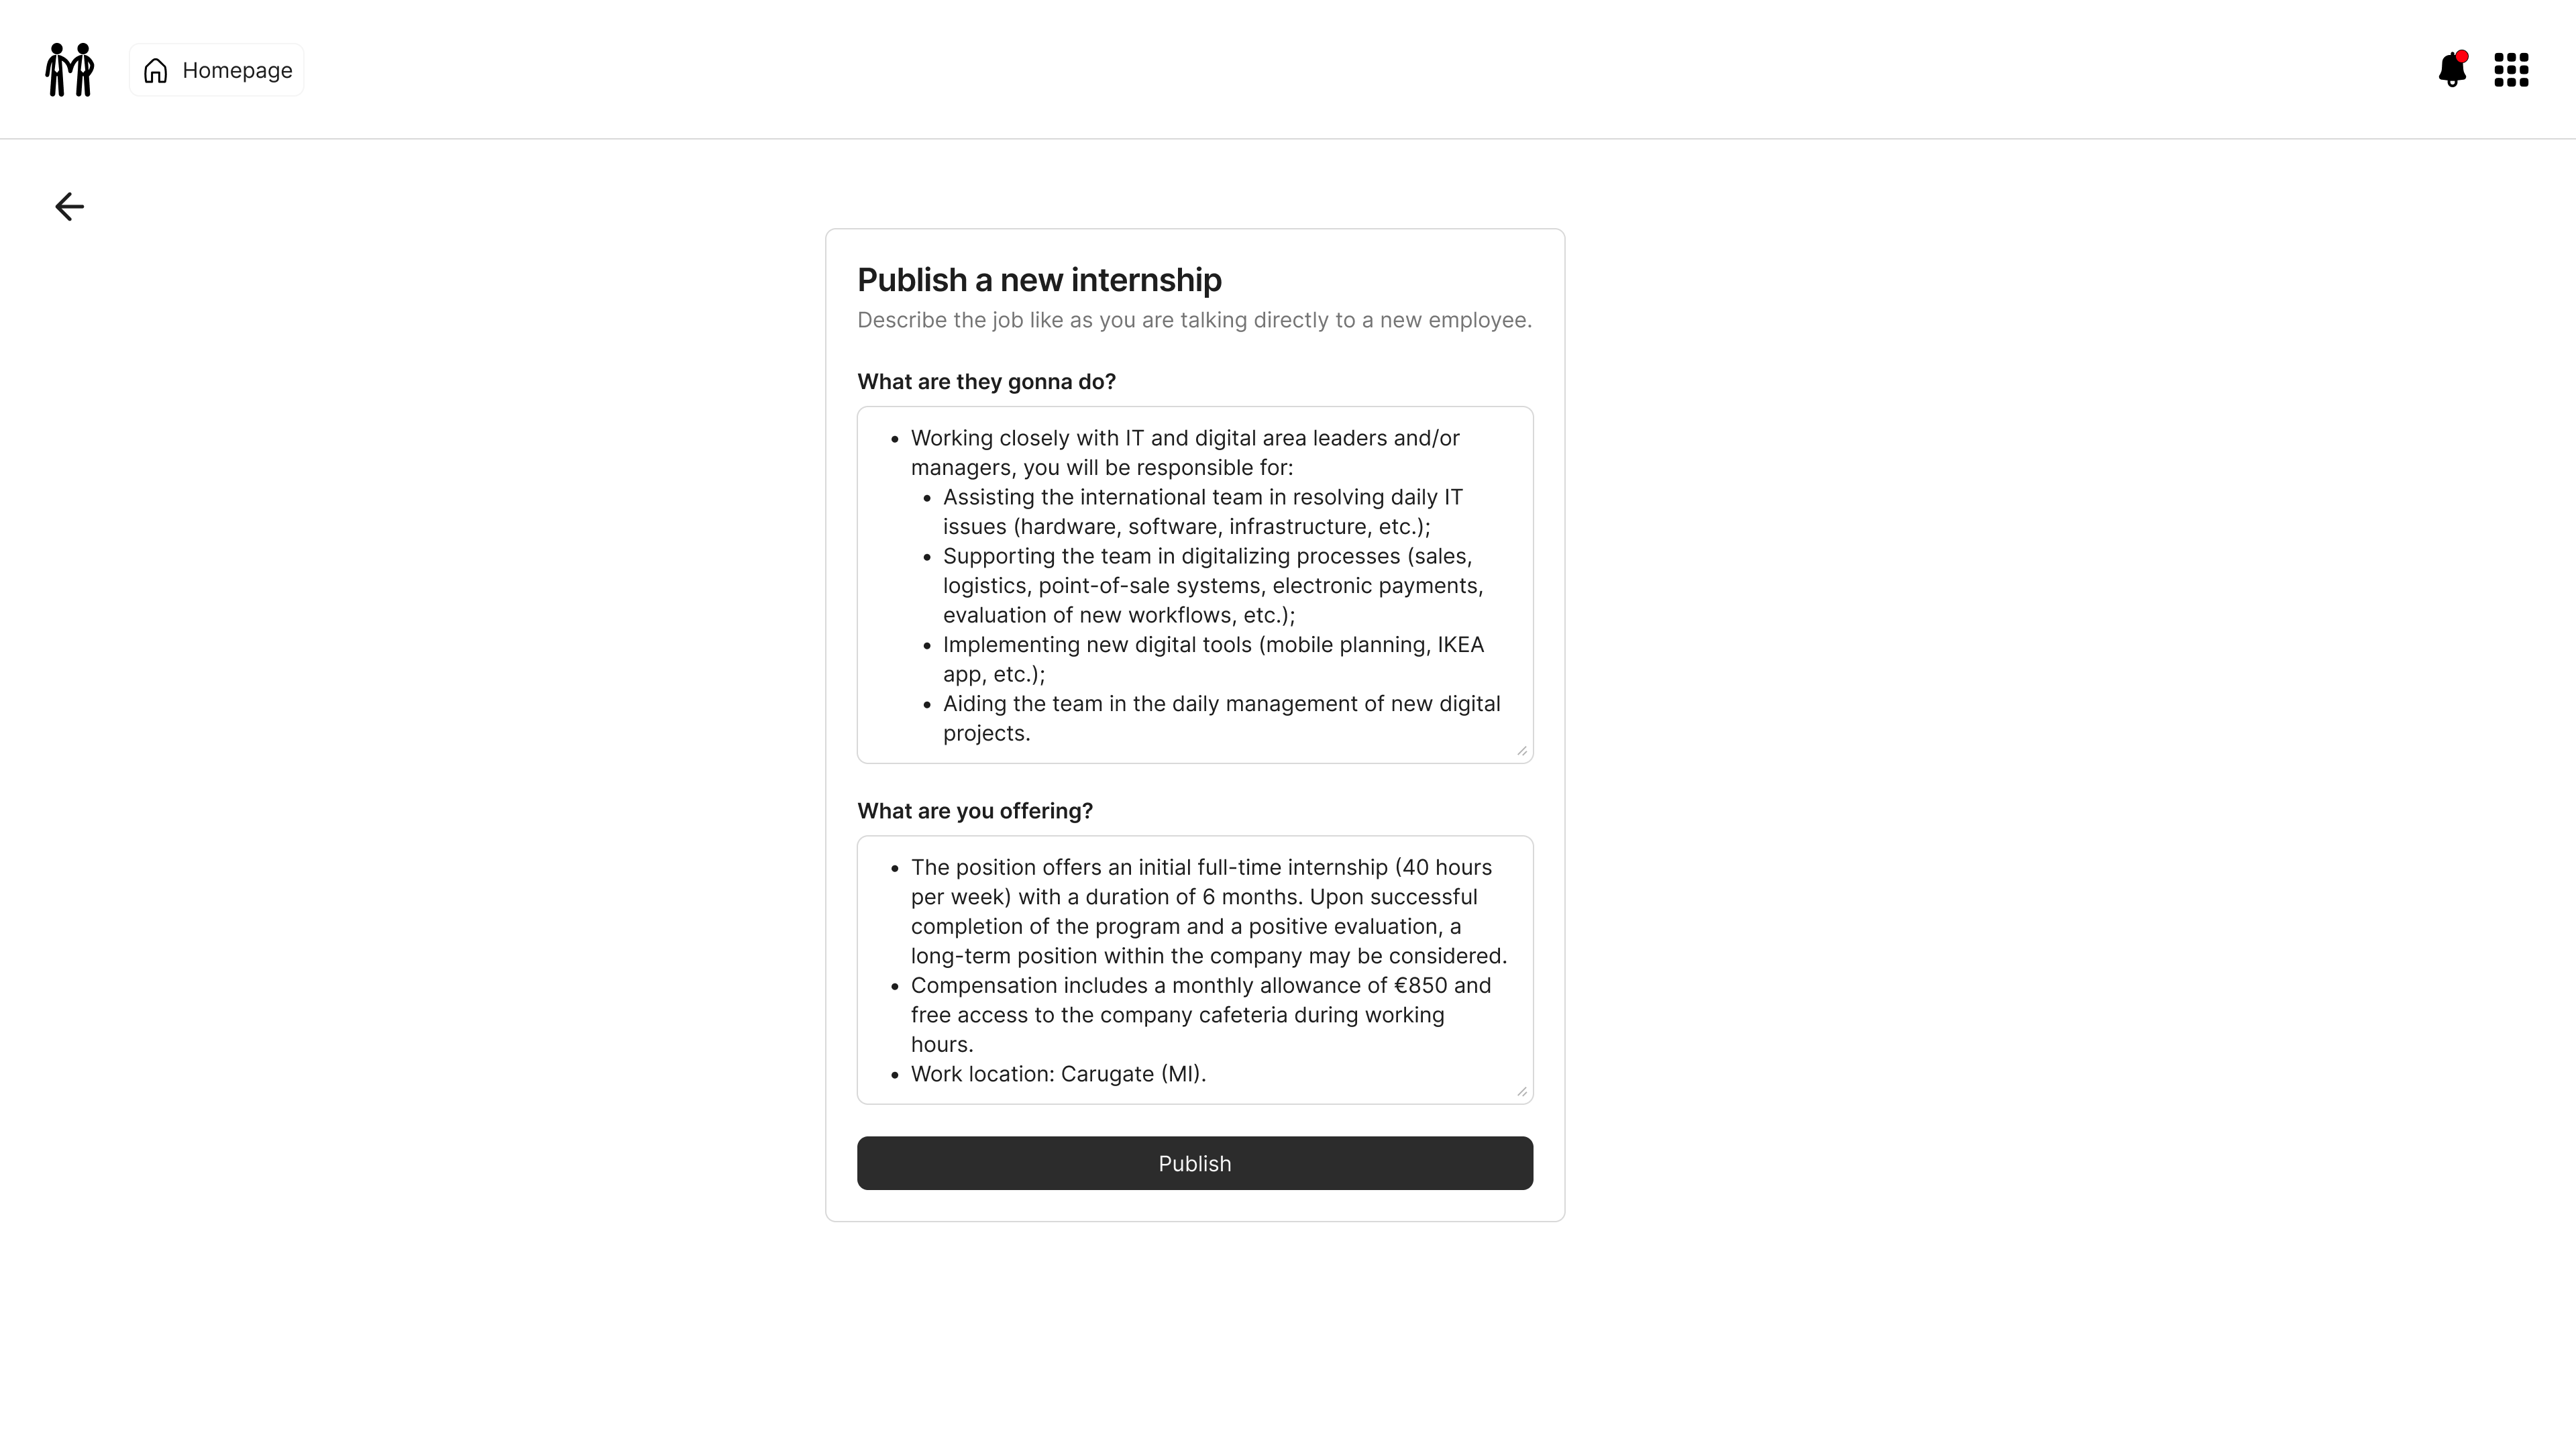
\includegraphics[width=1.0\textwidth]{Images/GUI/CO/Internship Creation - 2 - CO.png}}
    \caption{Internship Creation - 2 - CO}
    \label{fig:internship-creation-2-co}
\end{figure}

\par The Internship Creation page allows the CO to create a new internship. The CO is tasked to fill in all the
required information in order to post the internship on the platform.

\subsection{Internship Details - CO}
\label{subsec:internship-details-co}%

\begin{figure}[H]
    \centering
    \fbox{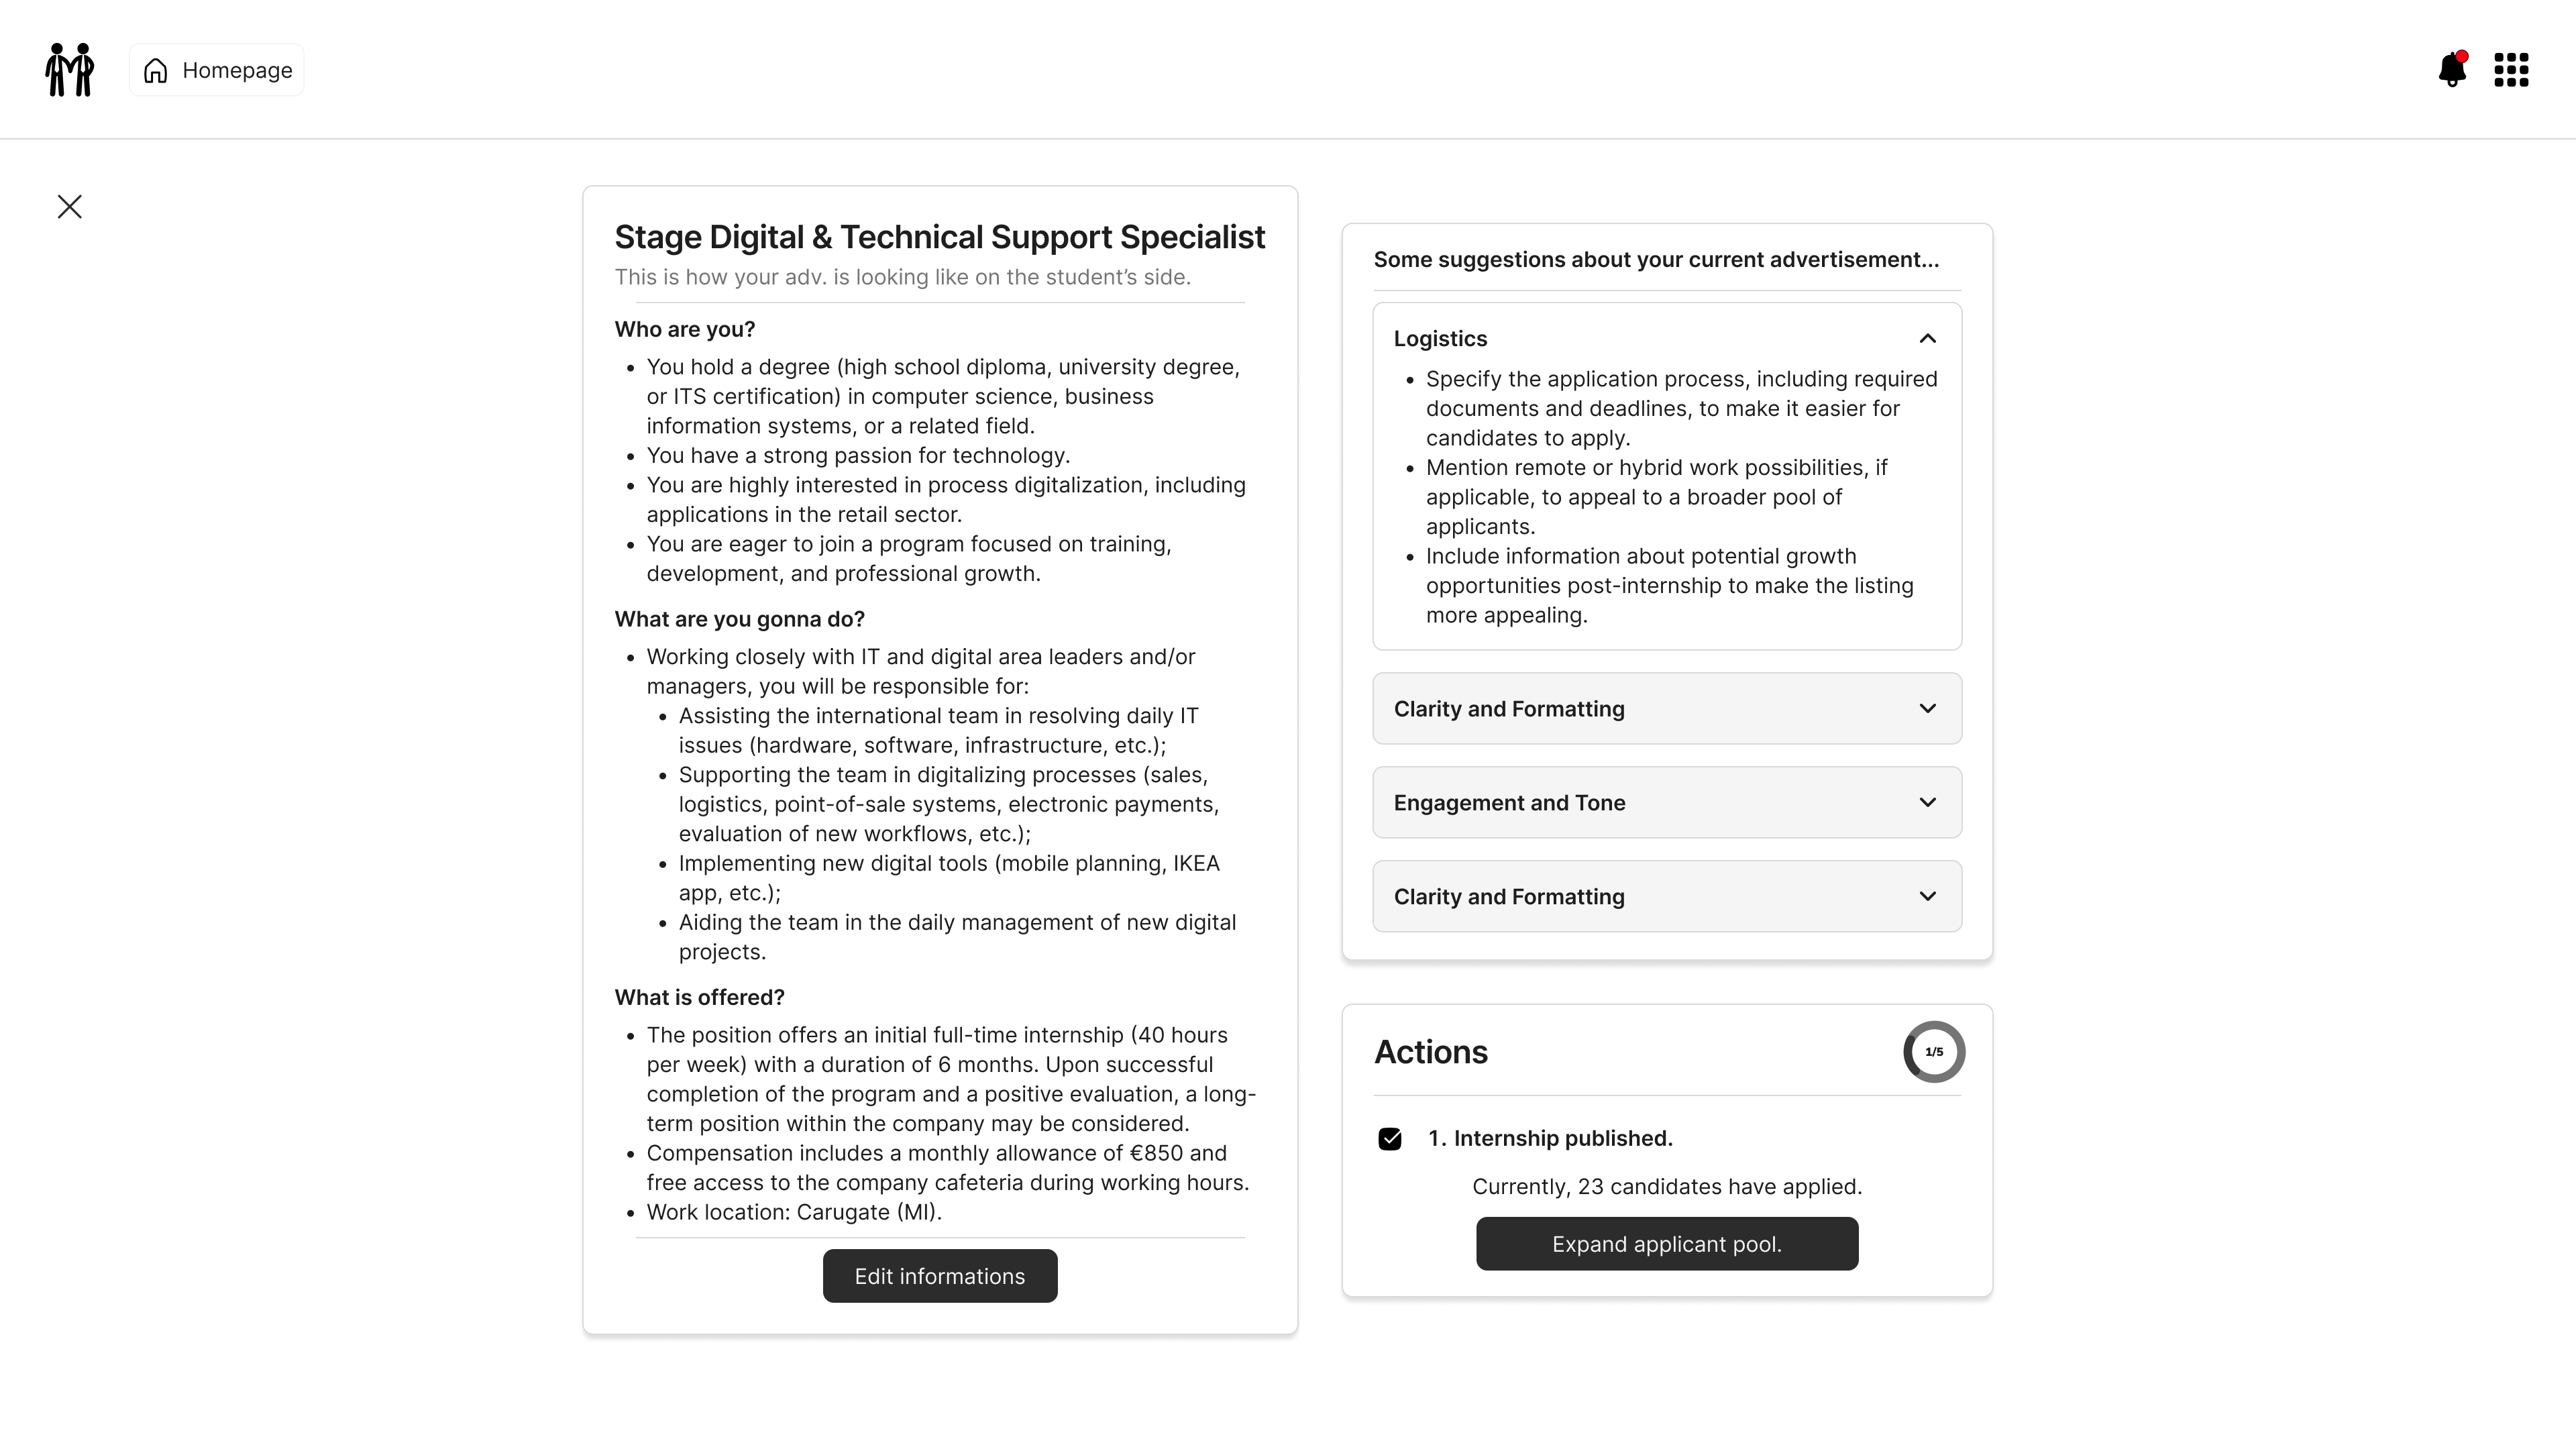
\includegraphics[width=1.0\textwidth]{Images/GUI/CO/Internship Published - Waiting for Applicants - CO.png}}
    \caption{Internship Details - 1 - CO}
    \label{fig:internship-creation-2-co}
\end{figure}

\par The Internship Details page will be presented in two critical stages divided by the application deadline. Before
the deadline the CO can not only edit the internship but also actively receive suggestions on how improve the
advertisement itself. After the deadline, the CO cannot edit the internship anymore in order to prevent abuse and
prevent confusion among the STs.

\par Also in this phase the CO can send notifications to the STs that the system has deemed as a good match for the
internship but have not applied yet. The CO can only view an anonymized version of the STs' profiles to prevent
information leakage. The interface used to select the STs will be shown later in the description of the "Request New
Applicants" page.

\begin{figure}[H]
    \centering
    \fbox{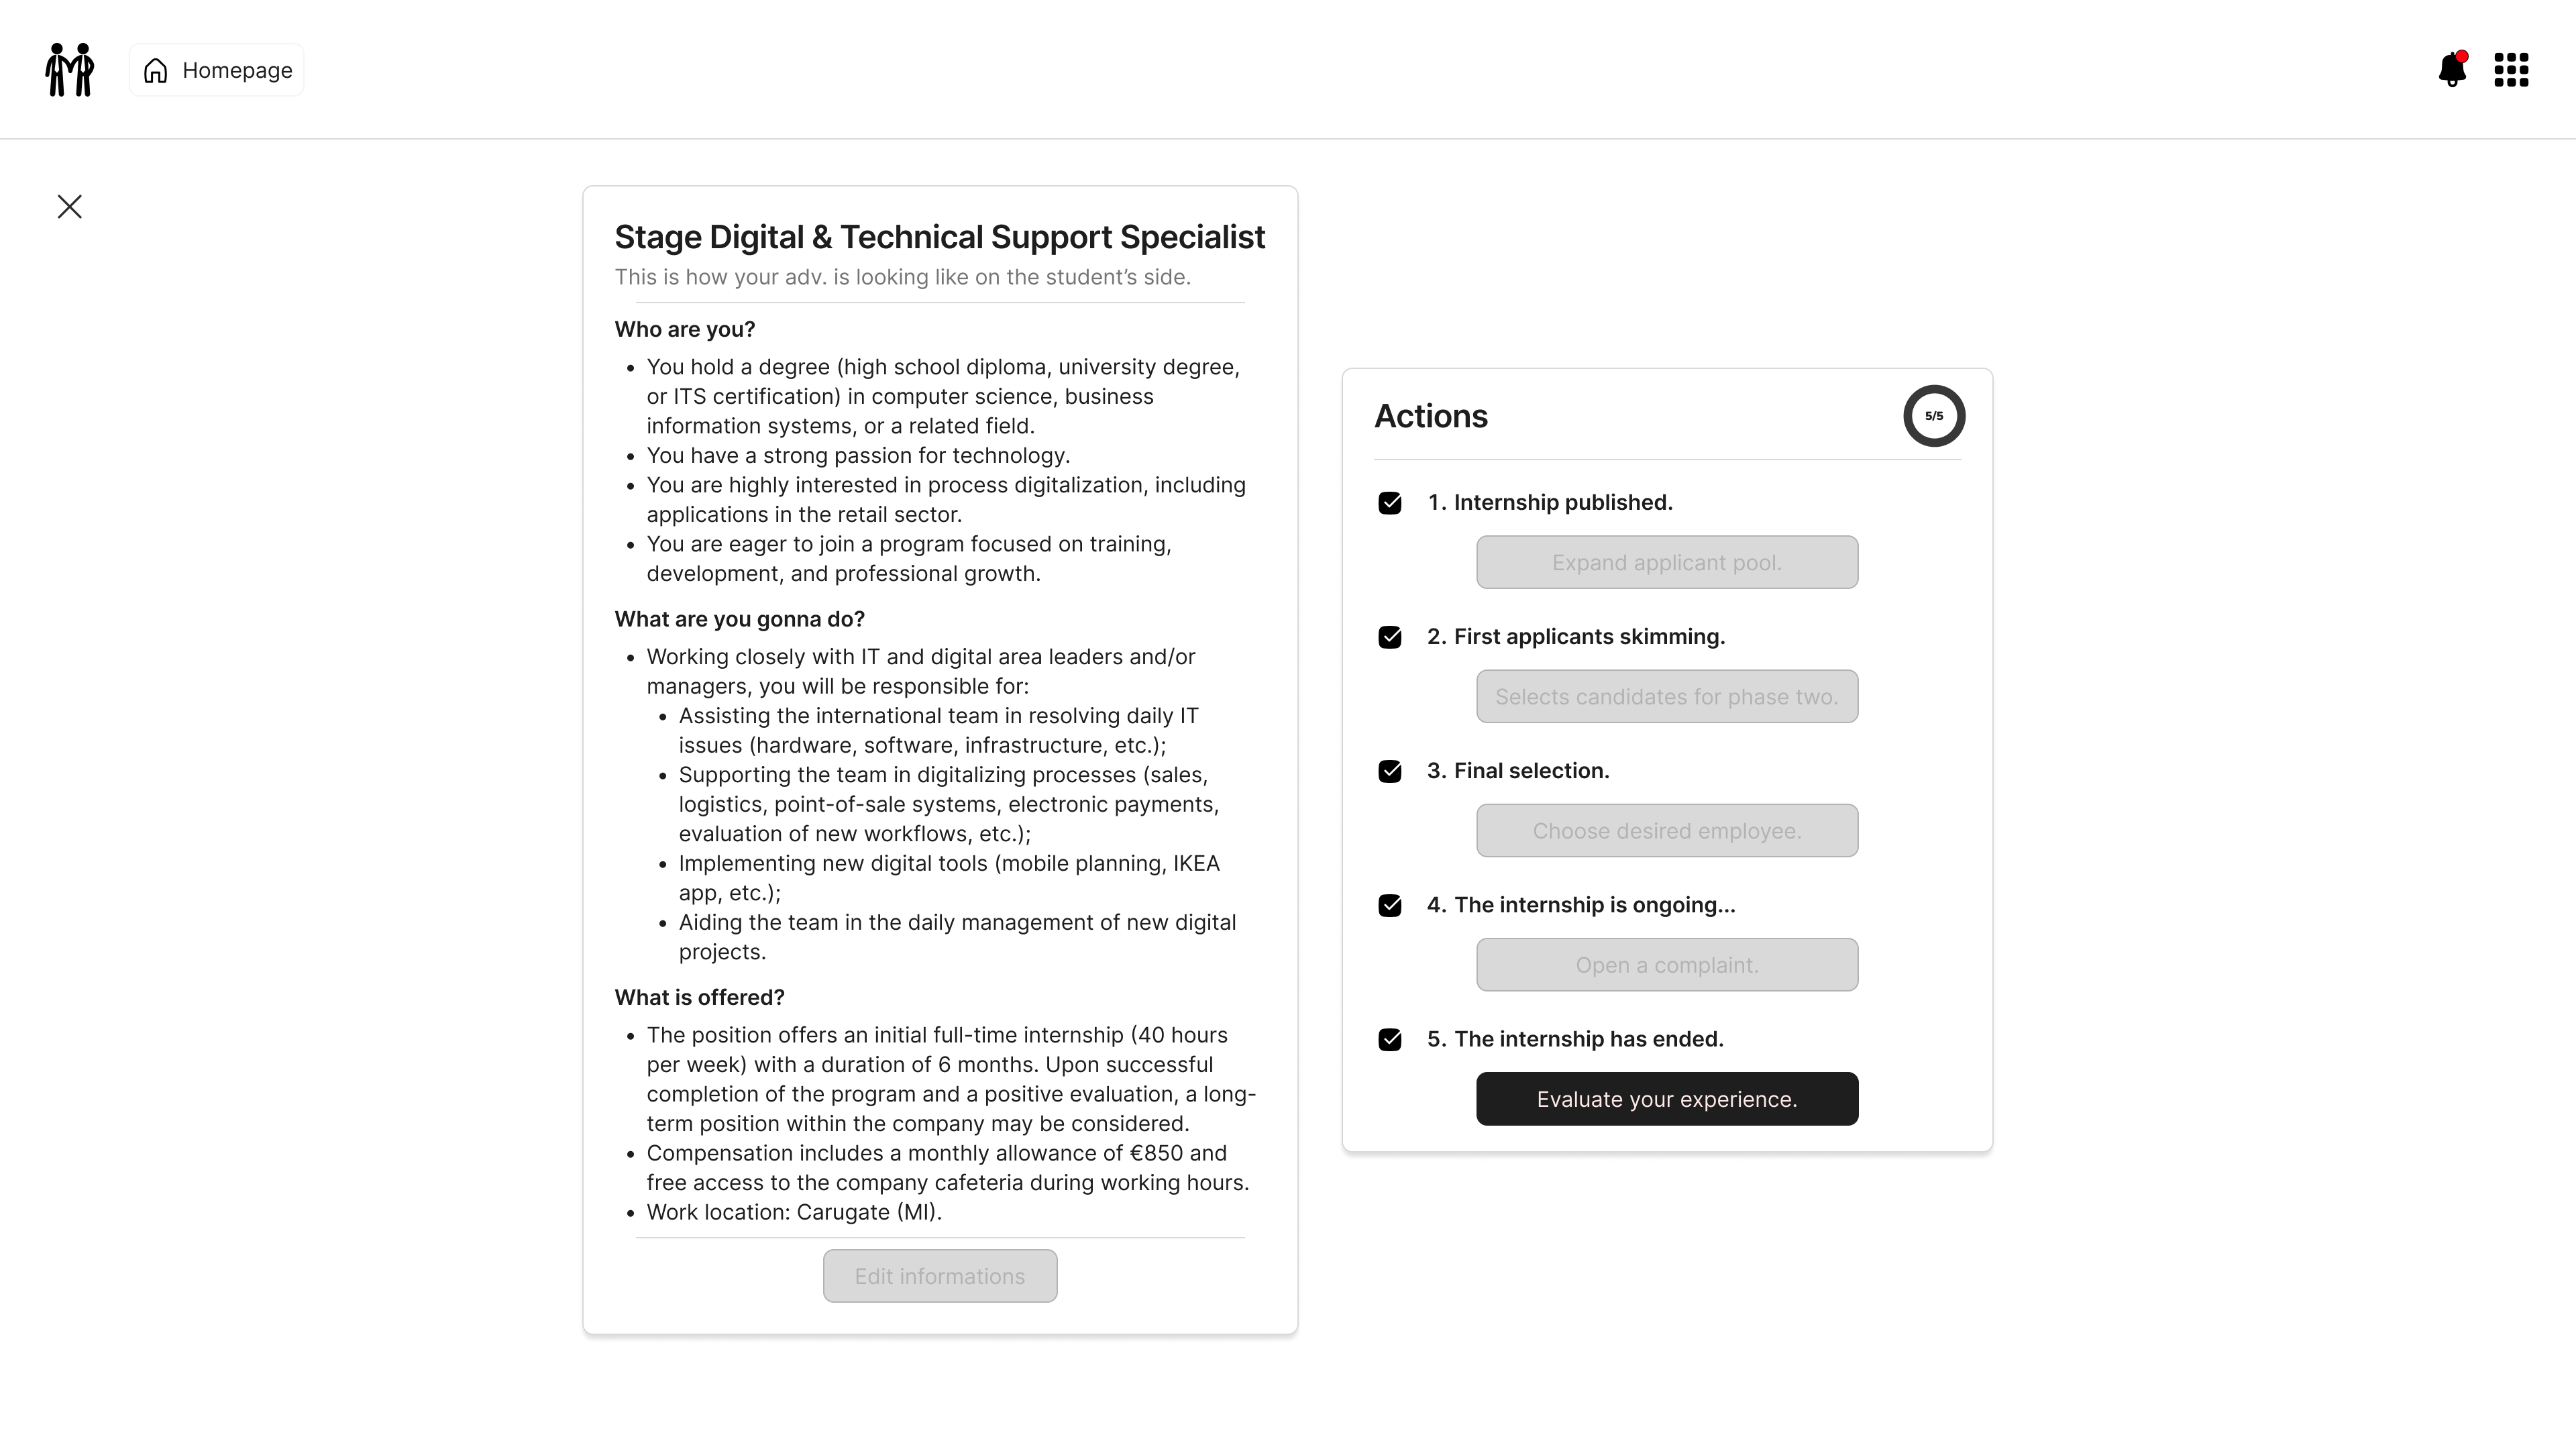
\includegraphics[width=1.0\textwidth]{Images/GUI/CO/Internship Published - Internship Completed - CO.png}}
    \caption{Internship Details - 1 - CO}
    \label{fig:internship-creation-2-co}
\end{figure}

\par As before, here is presented the page for a completed internship; the whole page evolution can easily be inferred
from this example.

\par Other that what has been already described, the CO can use this page - when appropriate - to request selected
STs to fill in the profiling questionnaire (Request Questionnaire), view the results of the questionnaire and select
the ST that will be hired (Select Employee), open a complaint if needed (Issue Reporting Form) and evaluate the
internship once it is over (Internship Feedback Survey).

\par The Internship Feedback Survey page and the Issue Reporting Form page are the same as the ones presented for the
ST and varies slightly only for the questions asked. For this reason, they will not be presented again.

\subsection{Request New Applicants - CO}
\label{subsec:request-new-applicants-co}%

\begin{figure}[H]
    \centering
    \fbox{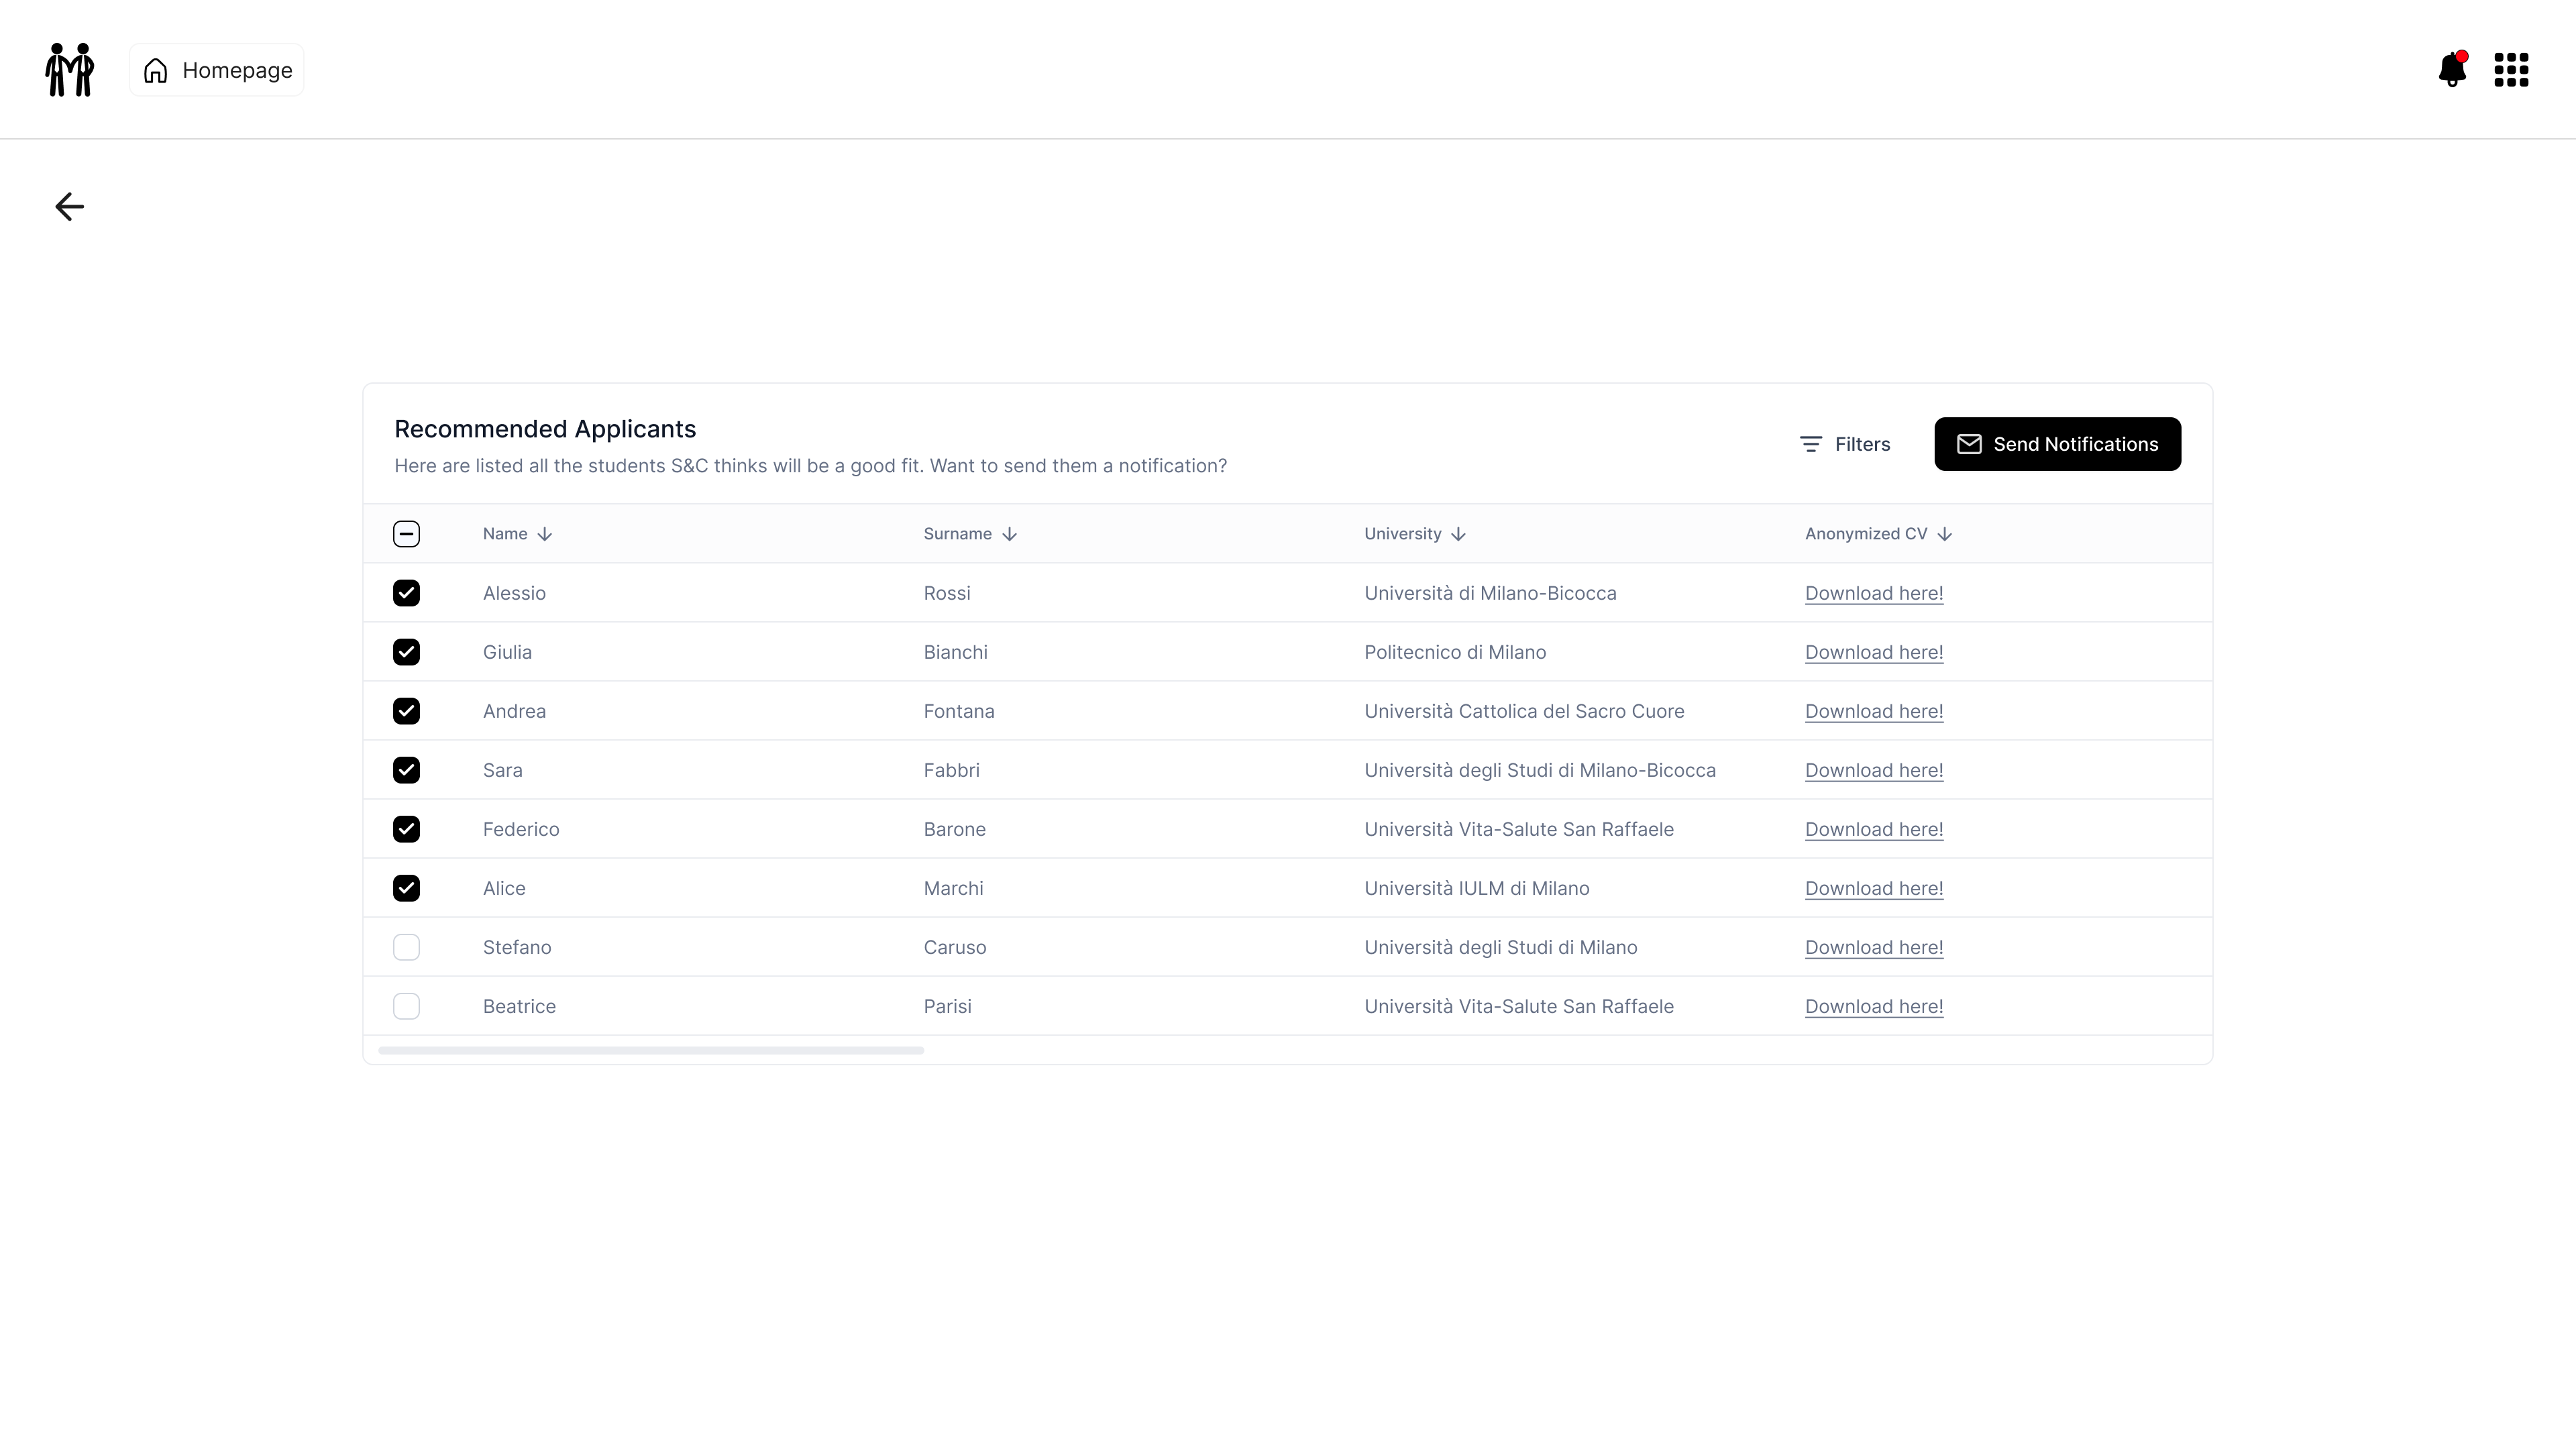
\includegraphics[width=1.0\textwidth]{Images/GUI/CO/Request New Applicants - CO.png}}
    \caption{Request New Applicants - CO}
    \label{fig:request-new-applicants-co}
\end{figure}

\par The Request New Applicants page allows the CO to send notifications to the STs that the system has deemed as a
good match for the internship but have not applied yet. These STs will maybe already have seen the internship thanks
to the system's suggestions but now we are showing them an active interest from the CO thus hoping to increase the
chances of them applying. The CO can only view an anonymized version of the STs' profiles to prevent information
leakage and abuse of the system: if the CO were able to see the full profiles of the STs, they could contact them
directly and bypass S\&C's system entirely.

\subsection{Request Questionnaire - CO}
\label{subsec:request-questionnaire-co}%

\begin{figure}[H]
    \centering
    \fbox{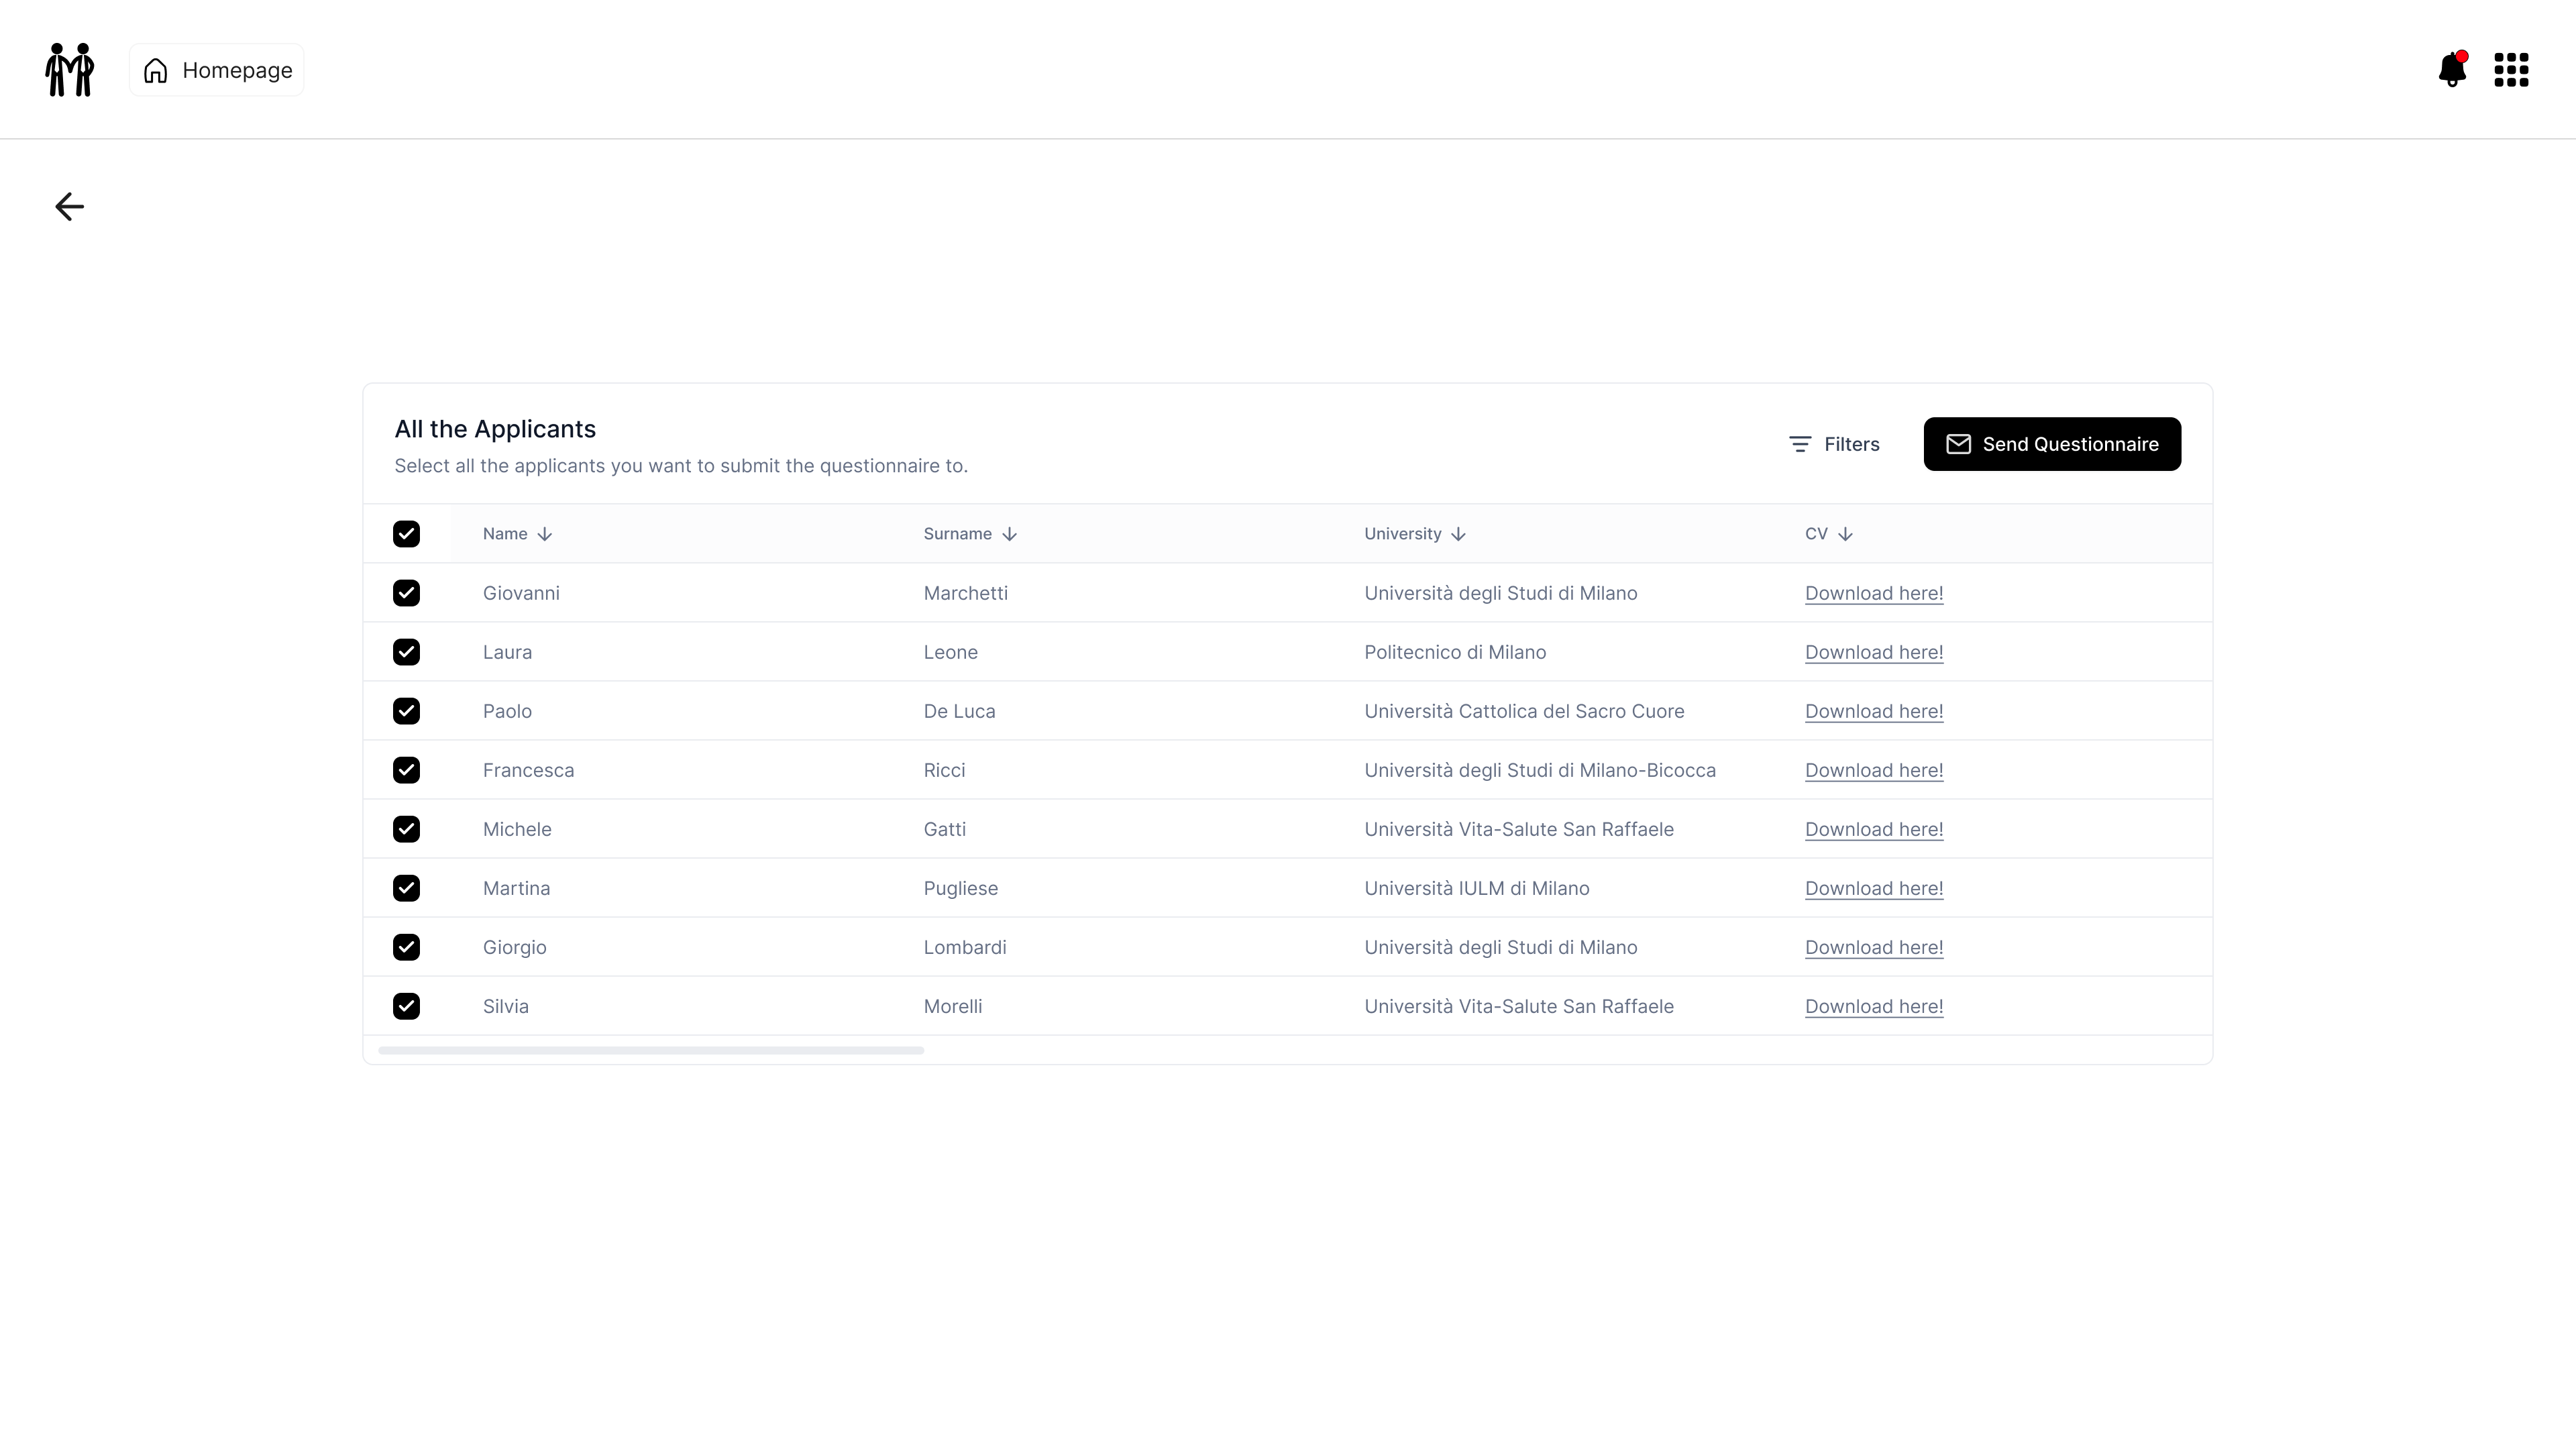
\includegraphics[width=1.0\textwidth]{Images/GUI/CO/Request Questionnaire - CO.png}}
    \caption{Request Questionnaire - CO}
    \label{fig:request-questionnaire-co}
\end{figure}

\par The Request Questionnaire page allows the CO to request the selected STs to fill in the profiling questionnaire.
Since the application deadline has passed - and the ST had already expressed their "consent" to be involved in this
internship - the CO can now see the full profiles of the STs.

\subsection{Select Employee - CO}
\label{subsec:select-employee-co}%

\begin{figure}[H]
    \centering
    \fbox{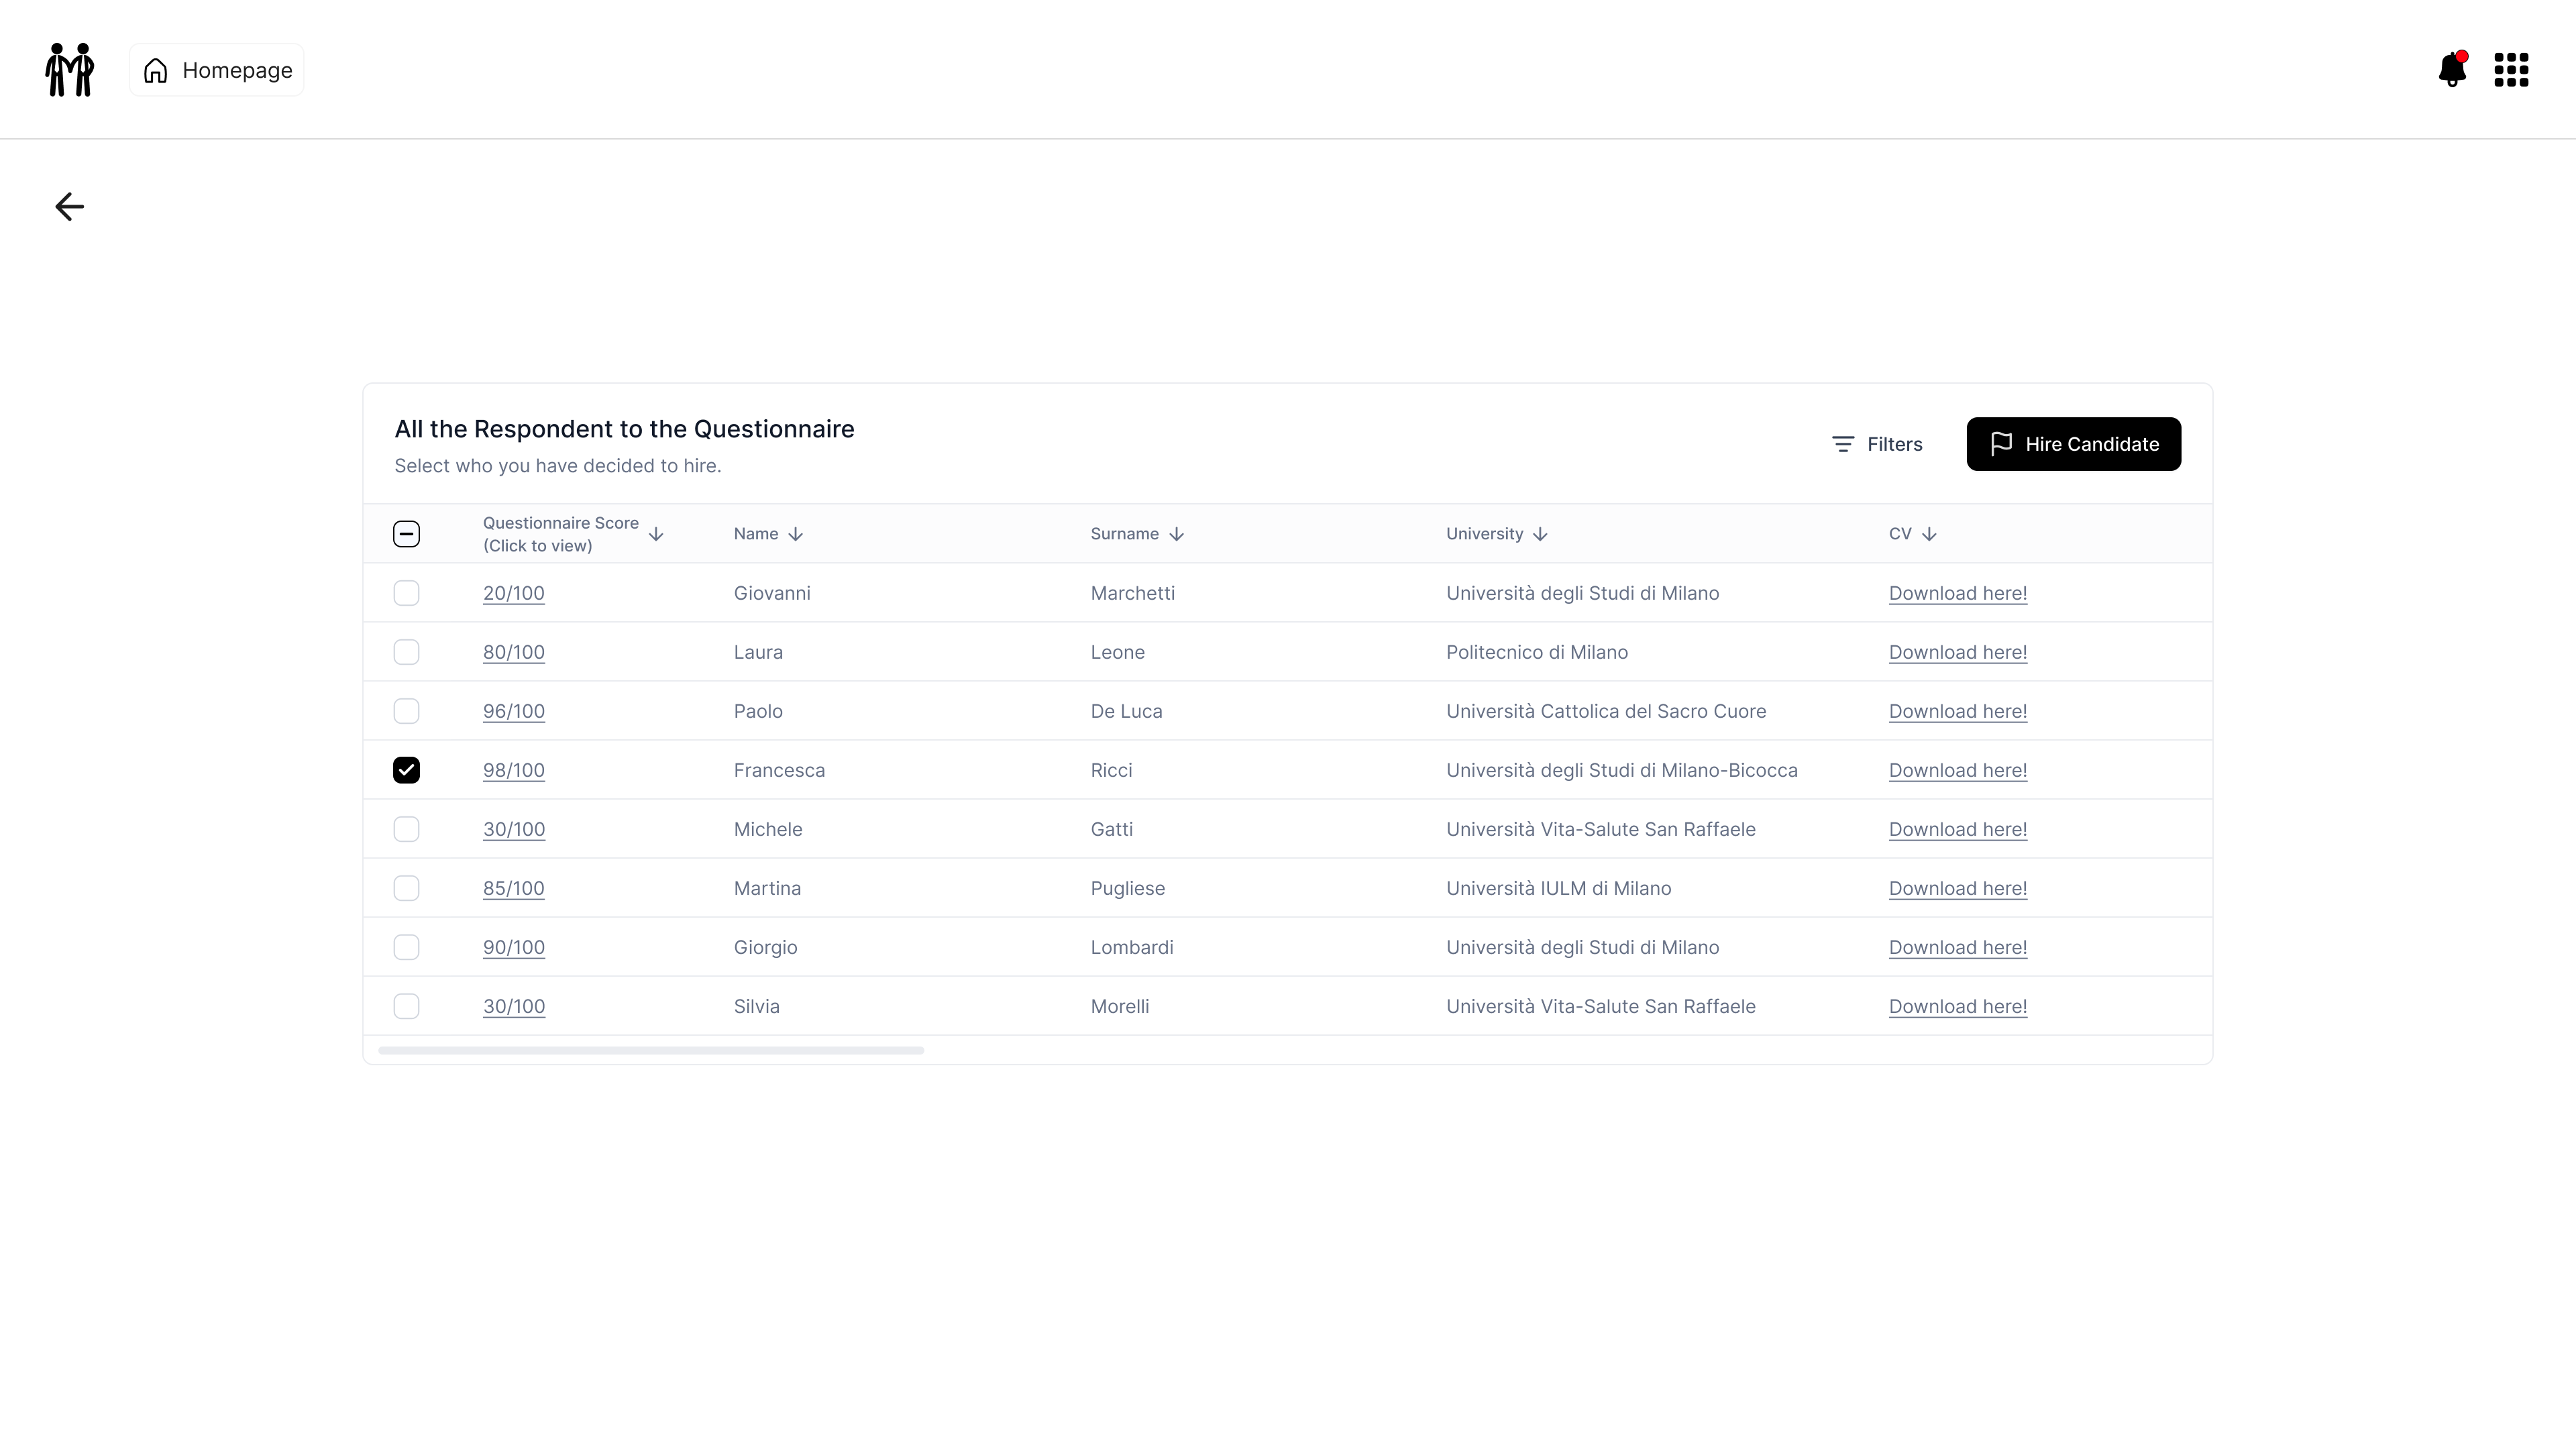
\includegraphics[width=1.0\textwidth]{Images/GUI/CO/Select Employee - CO.png}}
    \caption{Select Employee - CO}
    \label{fig:select-employee-co}
\end{figure}

\par The Select Employee page allows the CO to view the results of the questionnaire filled in by the STs and select
the ST that will be hired. This page is very similar to the Request Questionnaire page but with the addition of the
results of the questionnaire.

\section{"My Profile" - CO}
\label{subsec:profile-co}%

\begin{figure}[H]
    \centering
    \fbox{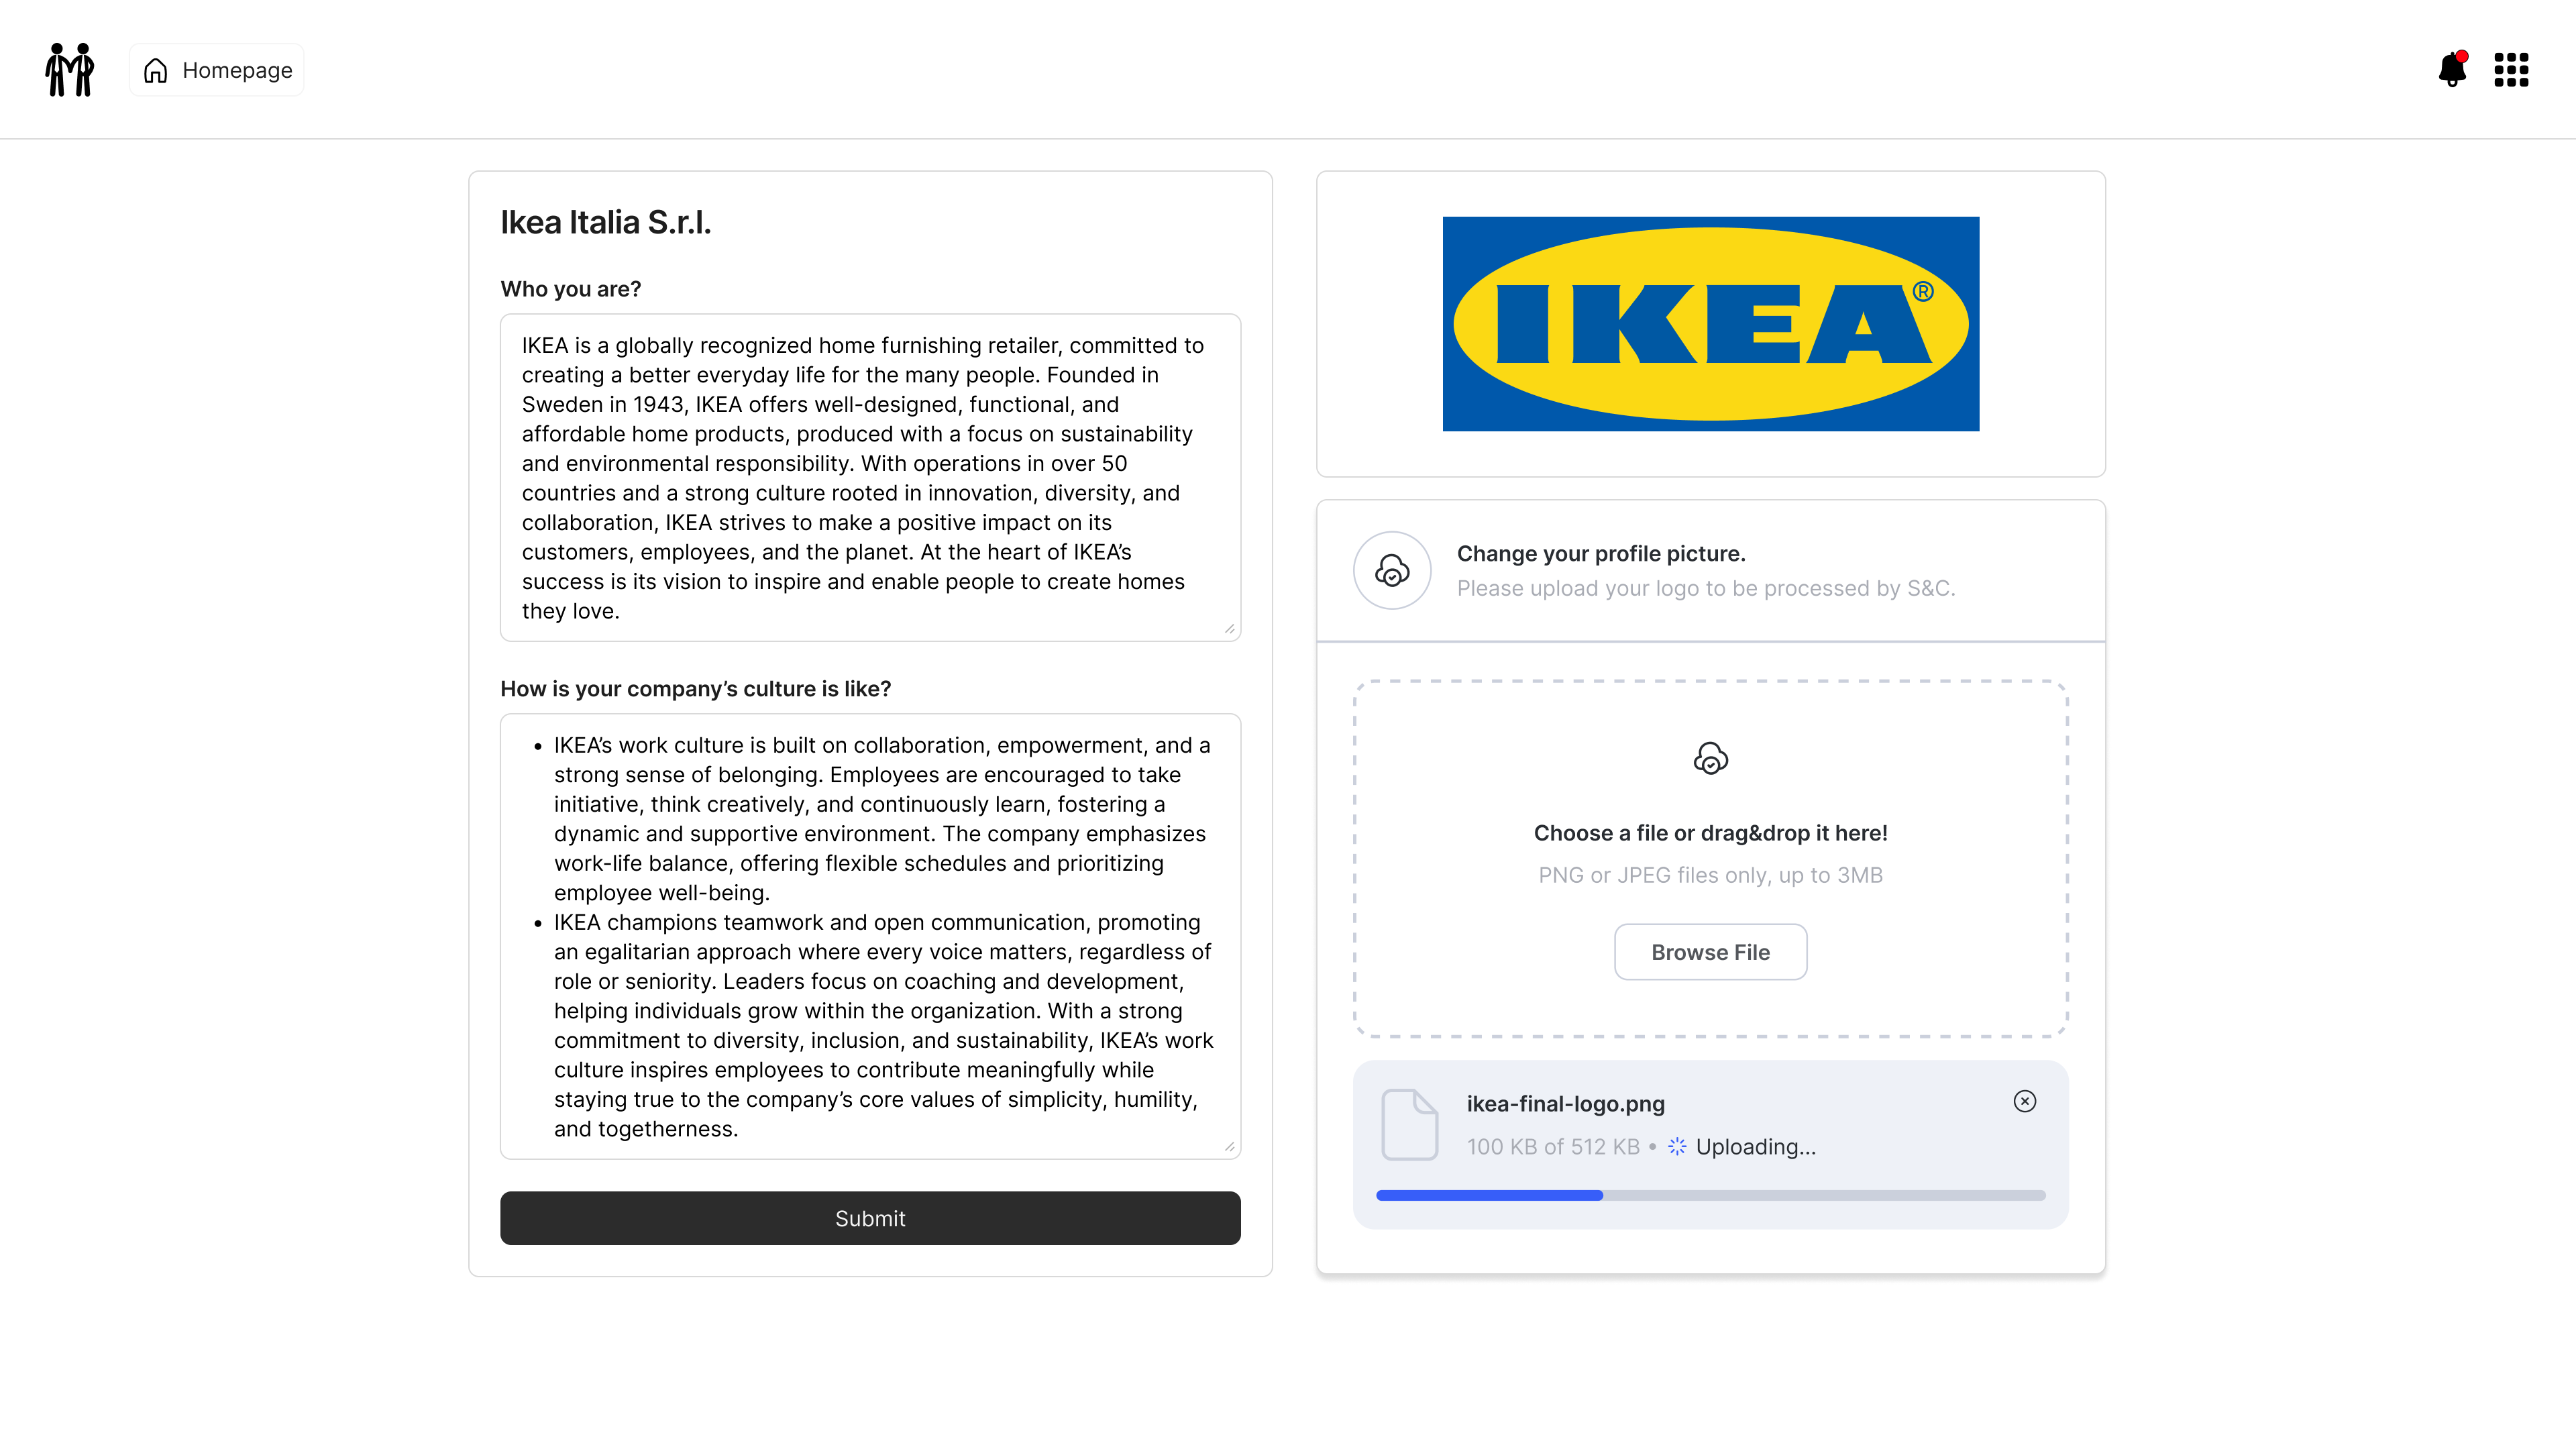
\includegraphics[width=1.0\textwidth]{Images/GUI/CO/Profile - CO.png}}
    \caption{"My Profile" - CO}
    \label{fig:profile-co}
\end{figure}

\par The "My Profile" page allows the CO to update their personal information. Along with the standard information,
this page offers the possibility to upload a the company's logo.

\section{User Flow: UN}
\label{sec:user-flow-un}%

\begin{figure}[H]
    \centering
    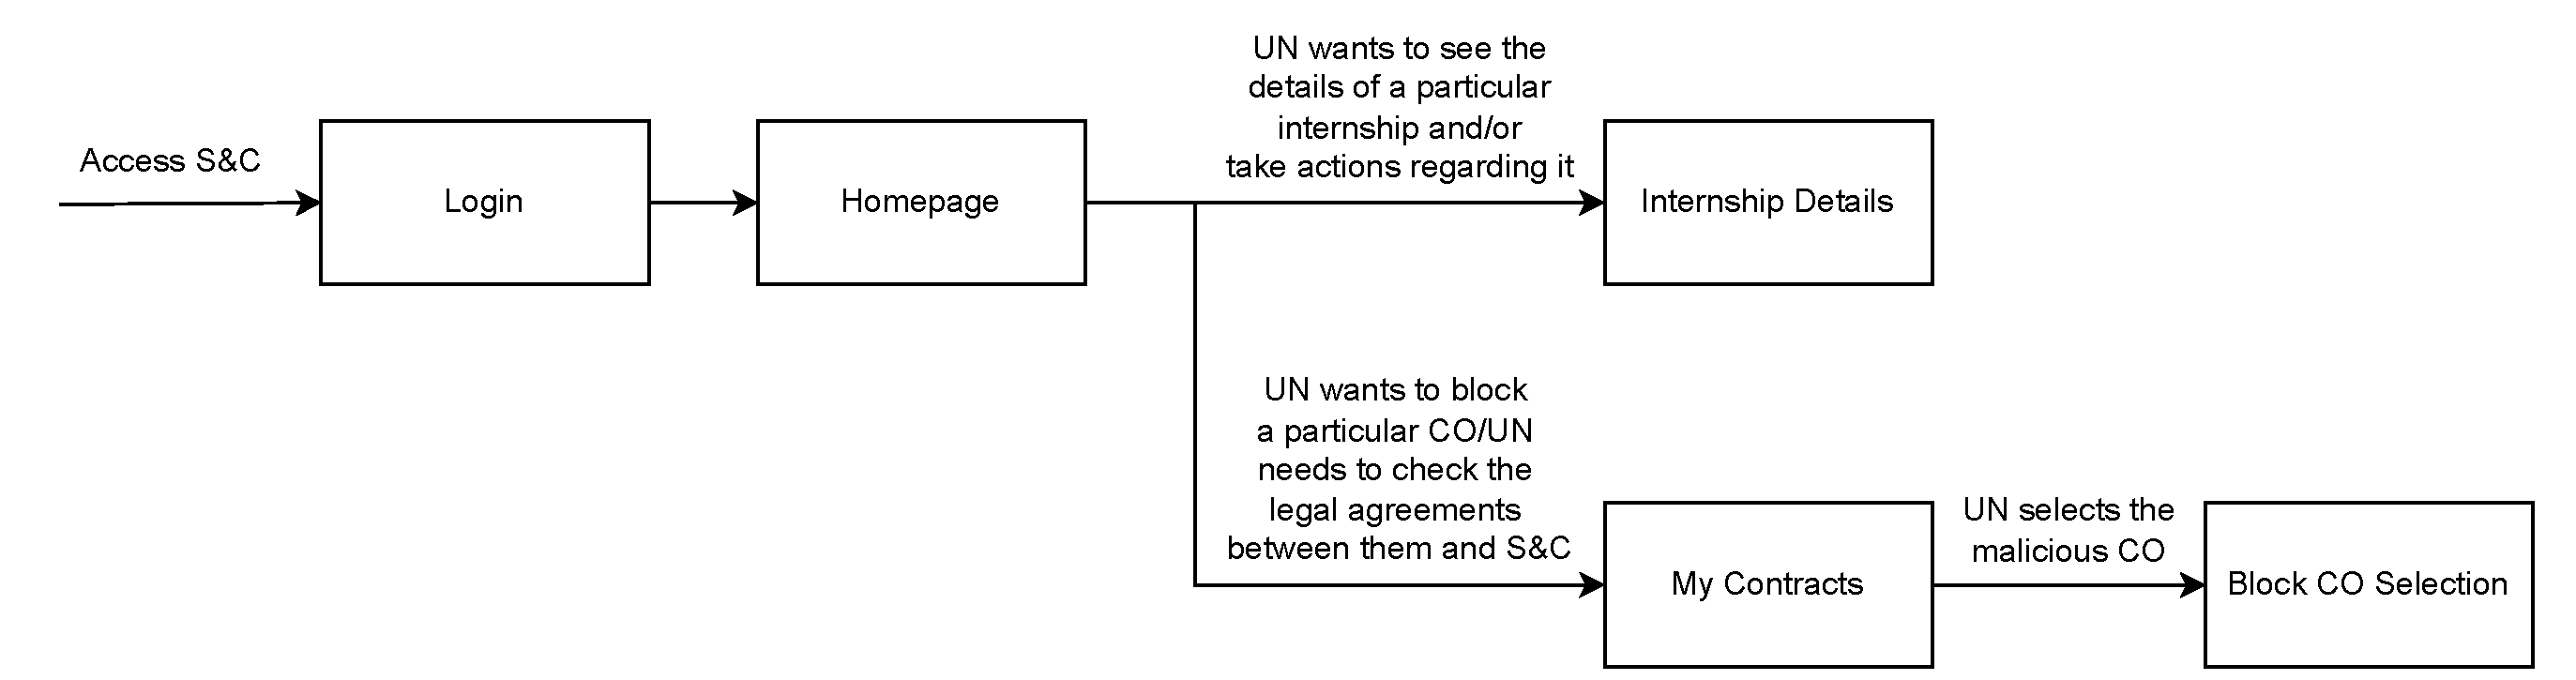
\includegraphics[width=1.0\textwidth]{Images/GUI/UN/Diagram.pdf}
    \caption{UN User Flow Diagram}
    \label{fig:un-user-flow-diagram}
\end{figure}

\par Here is presented the user flow diagram for the UN. The UN uses the Login page to authenticate and access S\&C and
then is redirected to the Homepage. On the Homepage, the UN can view all the internships that their students have
interacted with and the relative details (Internship Details). The Internship Details page will allow the UN: to view
all the details of an internship, view and answer to eventual complaints, and if needed, suspend the internship.

\par From the header, the UN can access the "My Contracts" page and log out of the system. In the "My Contracts" page,
the UN can view all the contracts that exist between the university and S\&C as well as block a malicious company.

\subsection{Homepage - UN}
\label{subsec:homepage-un}%

\begin{figure}[H]
    \centering
    \fbox{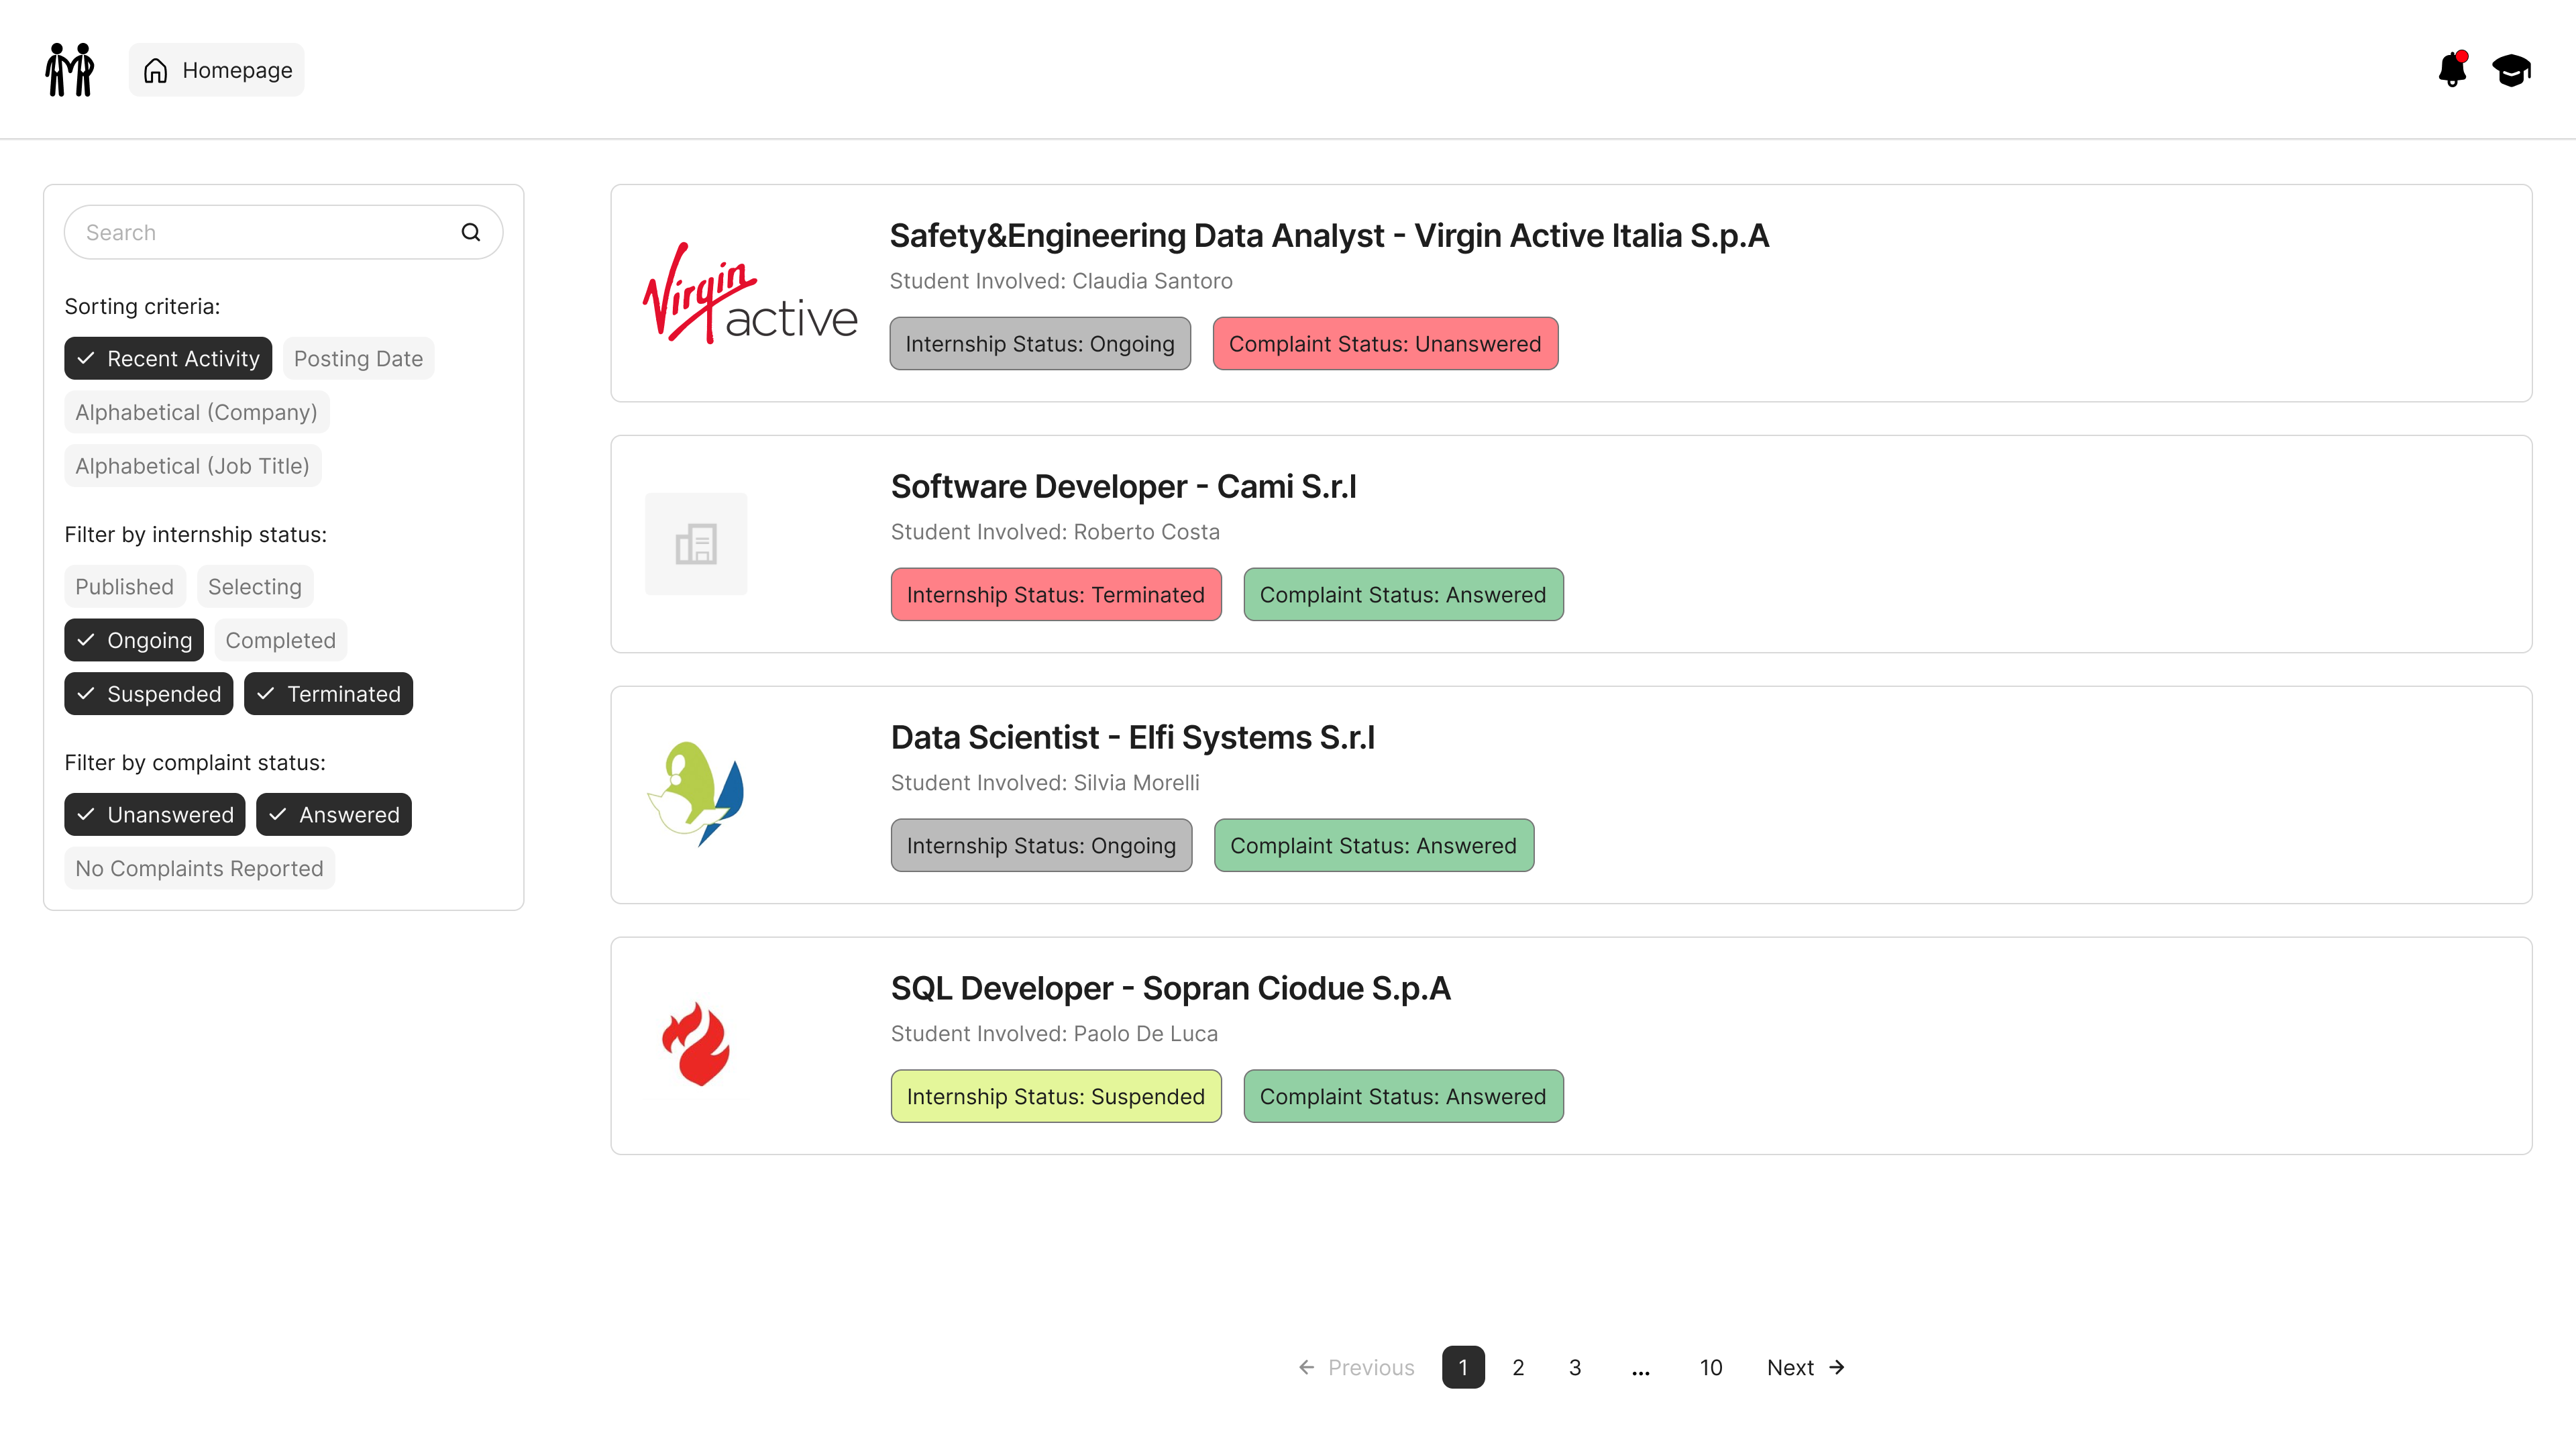
\includegraphics[width=1.0\textwidth]{Images/GUI/UN/Homepage - UN.png}}
    \caption{Homepage - UN}
    \label{fig:homepage-un}
\end{figure}

\par The Homepage is the main page for the UN. Here the user can view all the internships that their students have
interacted with and the relative details. Proper filters are provided to allow the user to search for internships based
on their preferences and needs.

\par As all the other pages, the header is present and allows the user to: access the "My Contracts" page, log out from
the platform and view any new notifications from the related submenu.

\begin{figure}[H]
    \centering
    \fbox{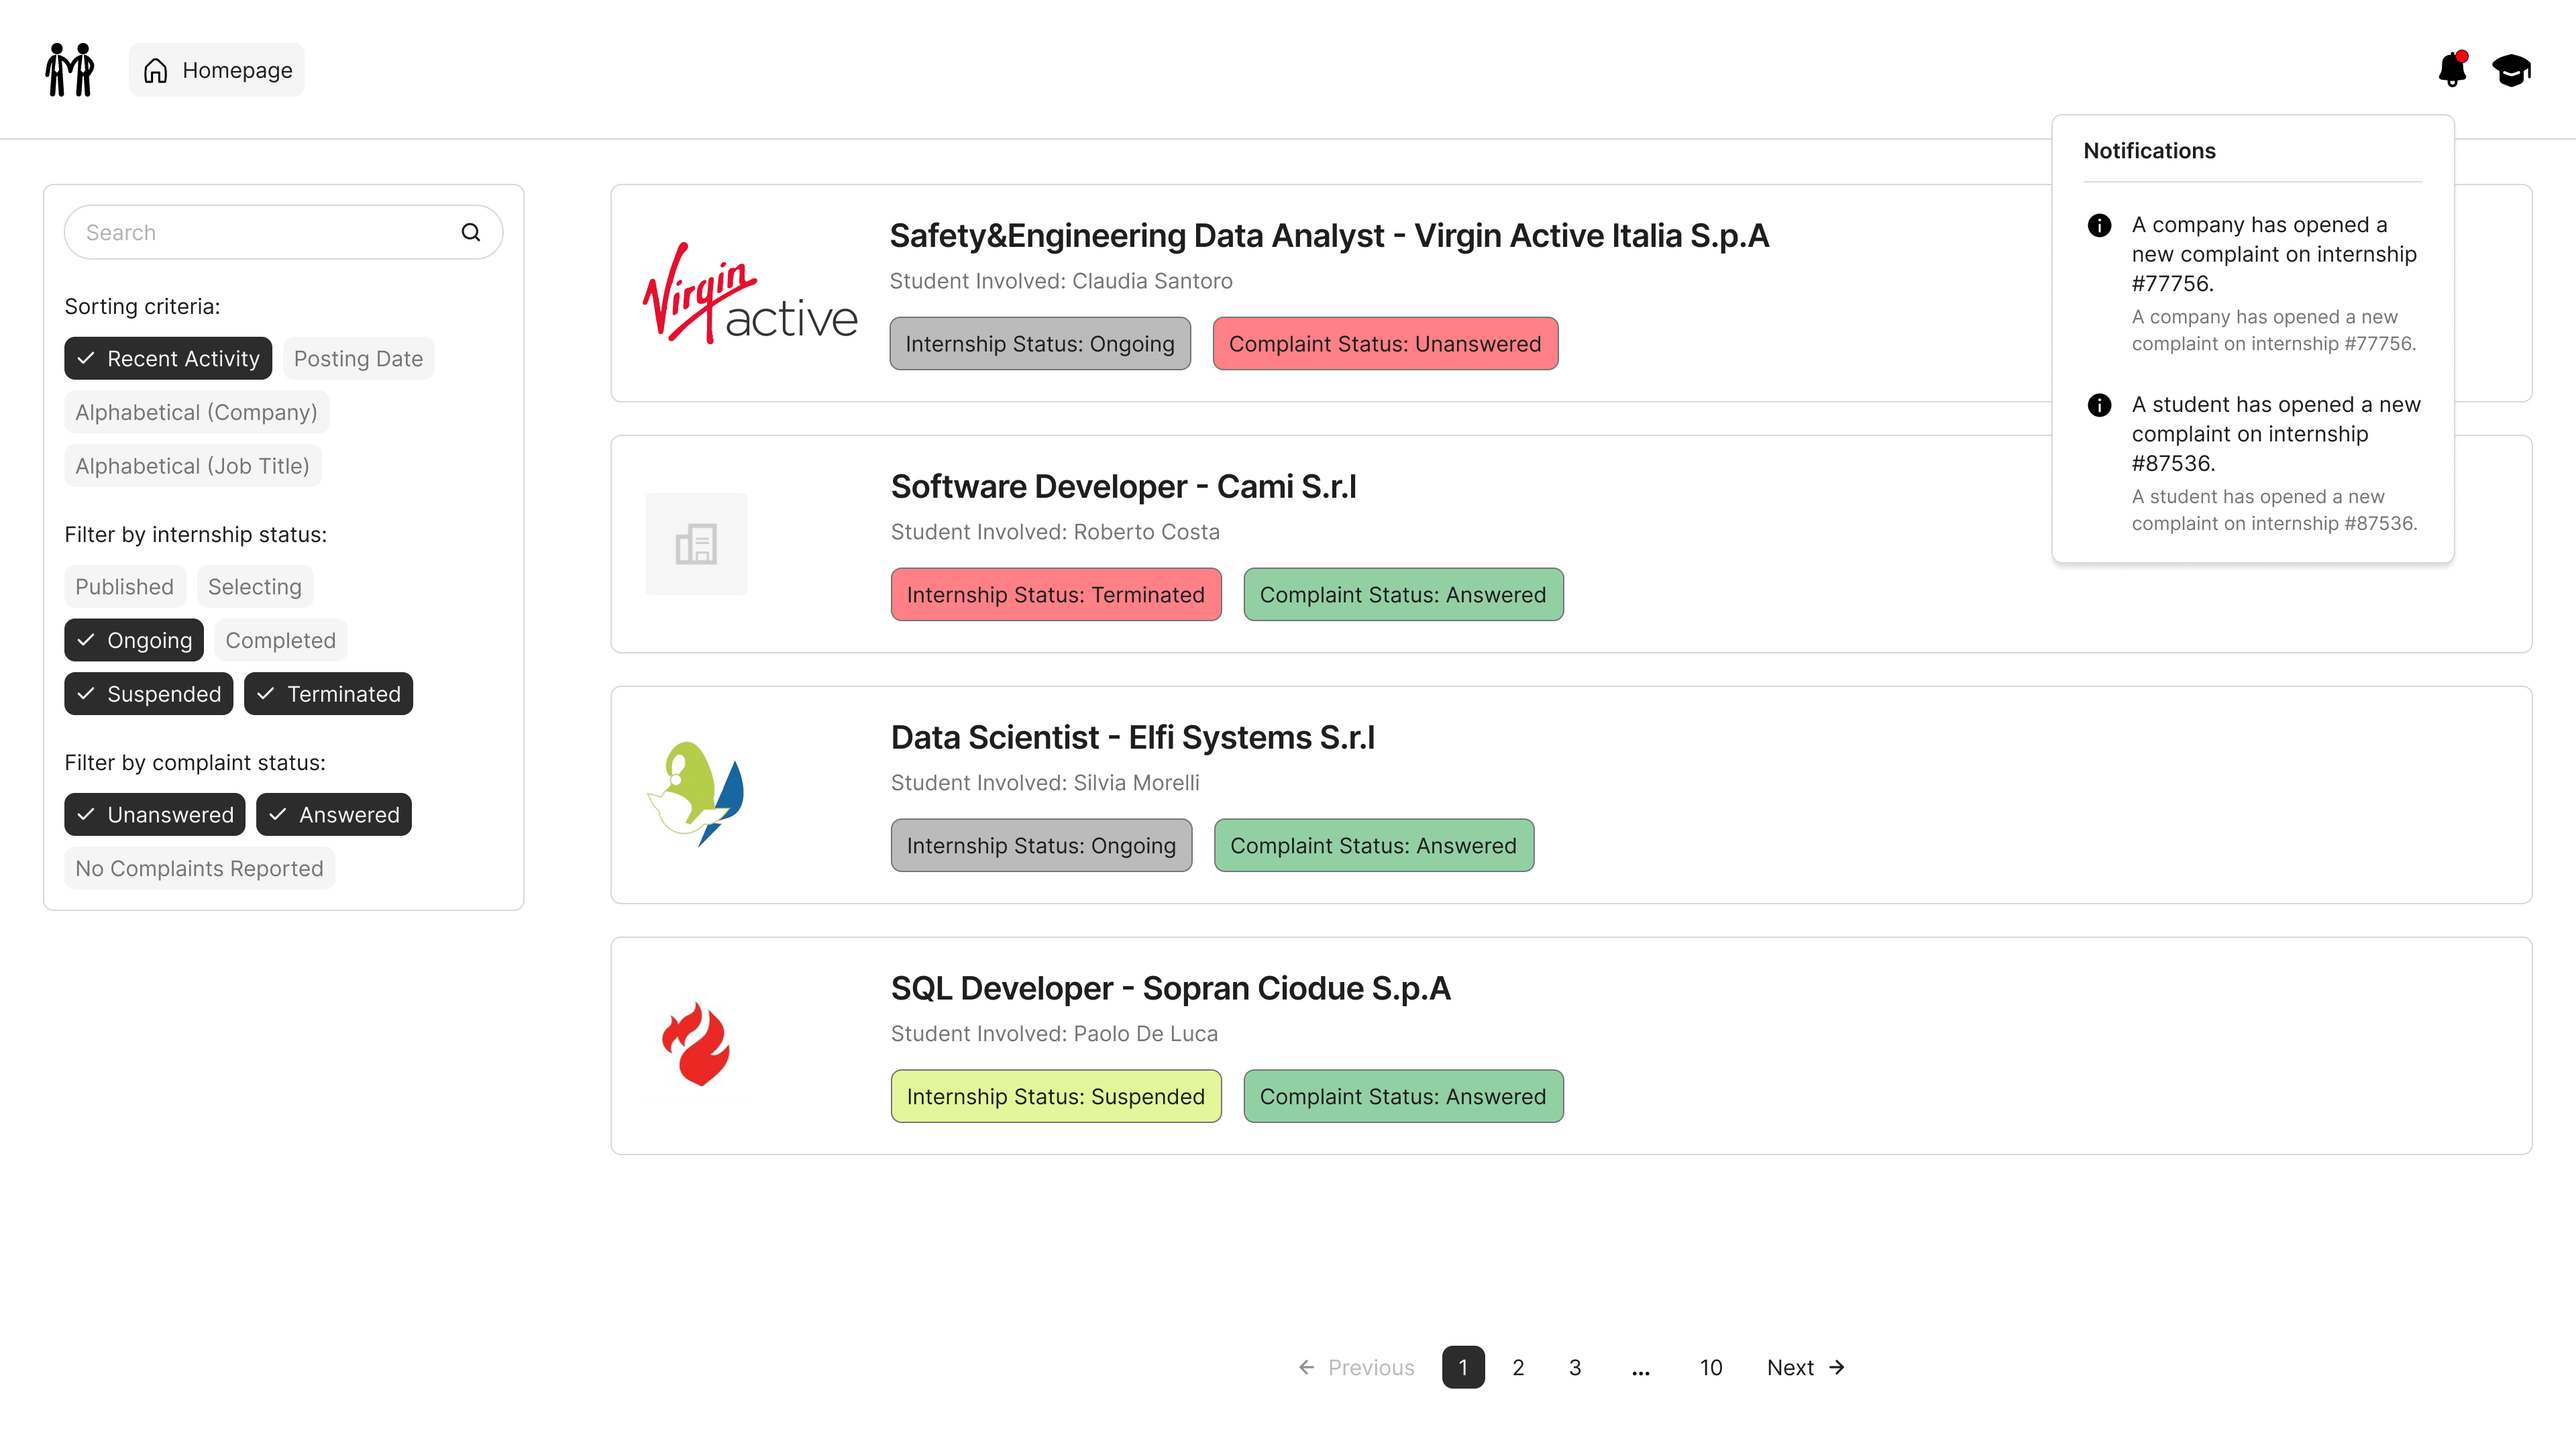
\includegraphics[width=1.0\textwidth]{Images/GUI/UN/Homepage - Notification - UN.png}}
    \caption{Homepage - UN - Notification}
    \label{fig:homepage-un-notification}
\end{figure}

\begin{figure}[H]
    \centering
    \fbox{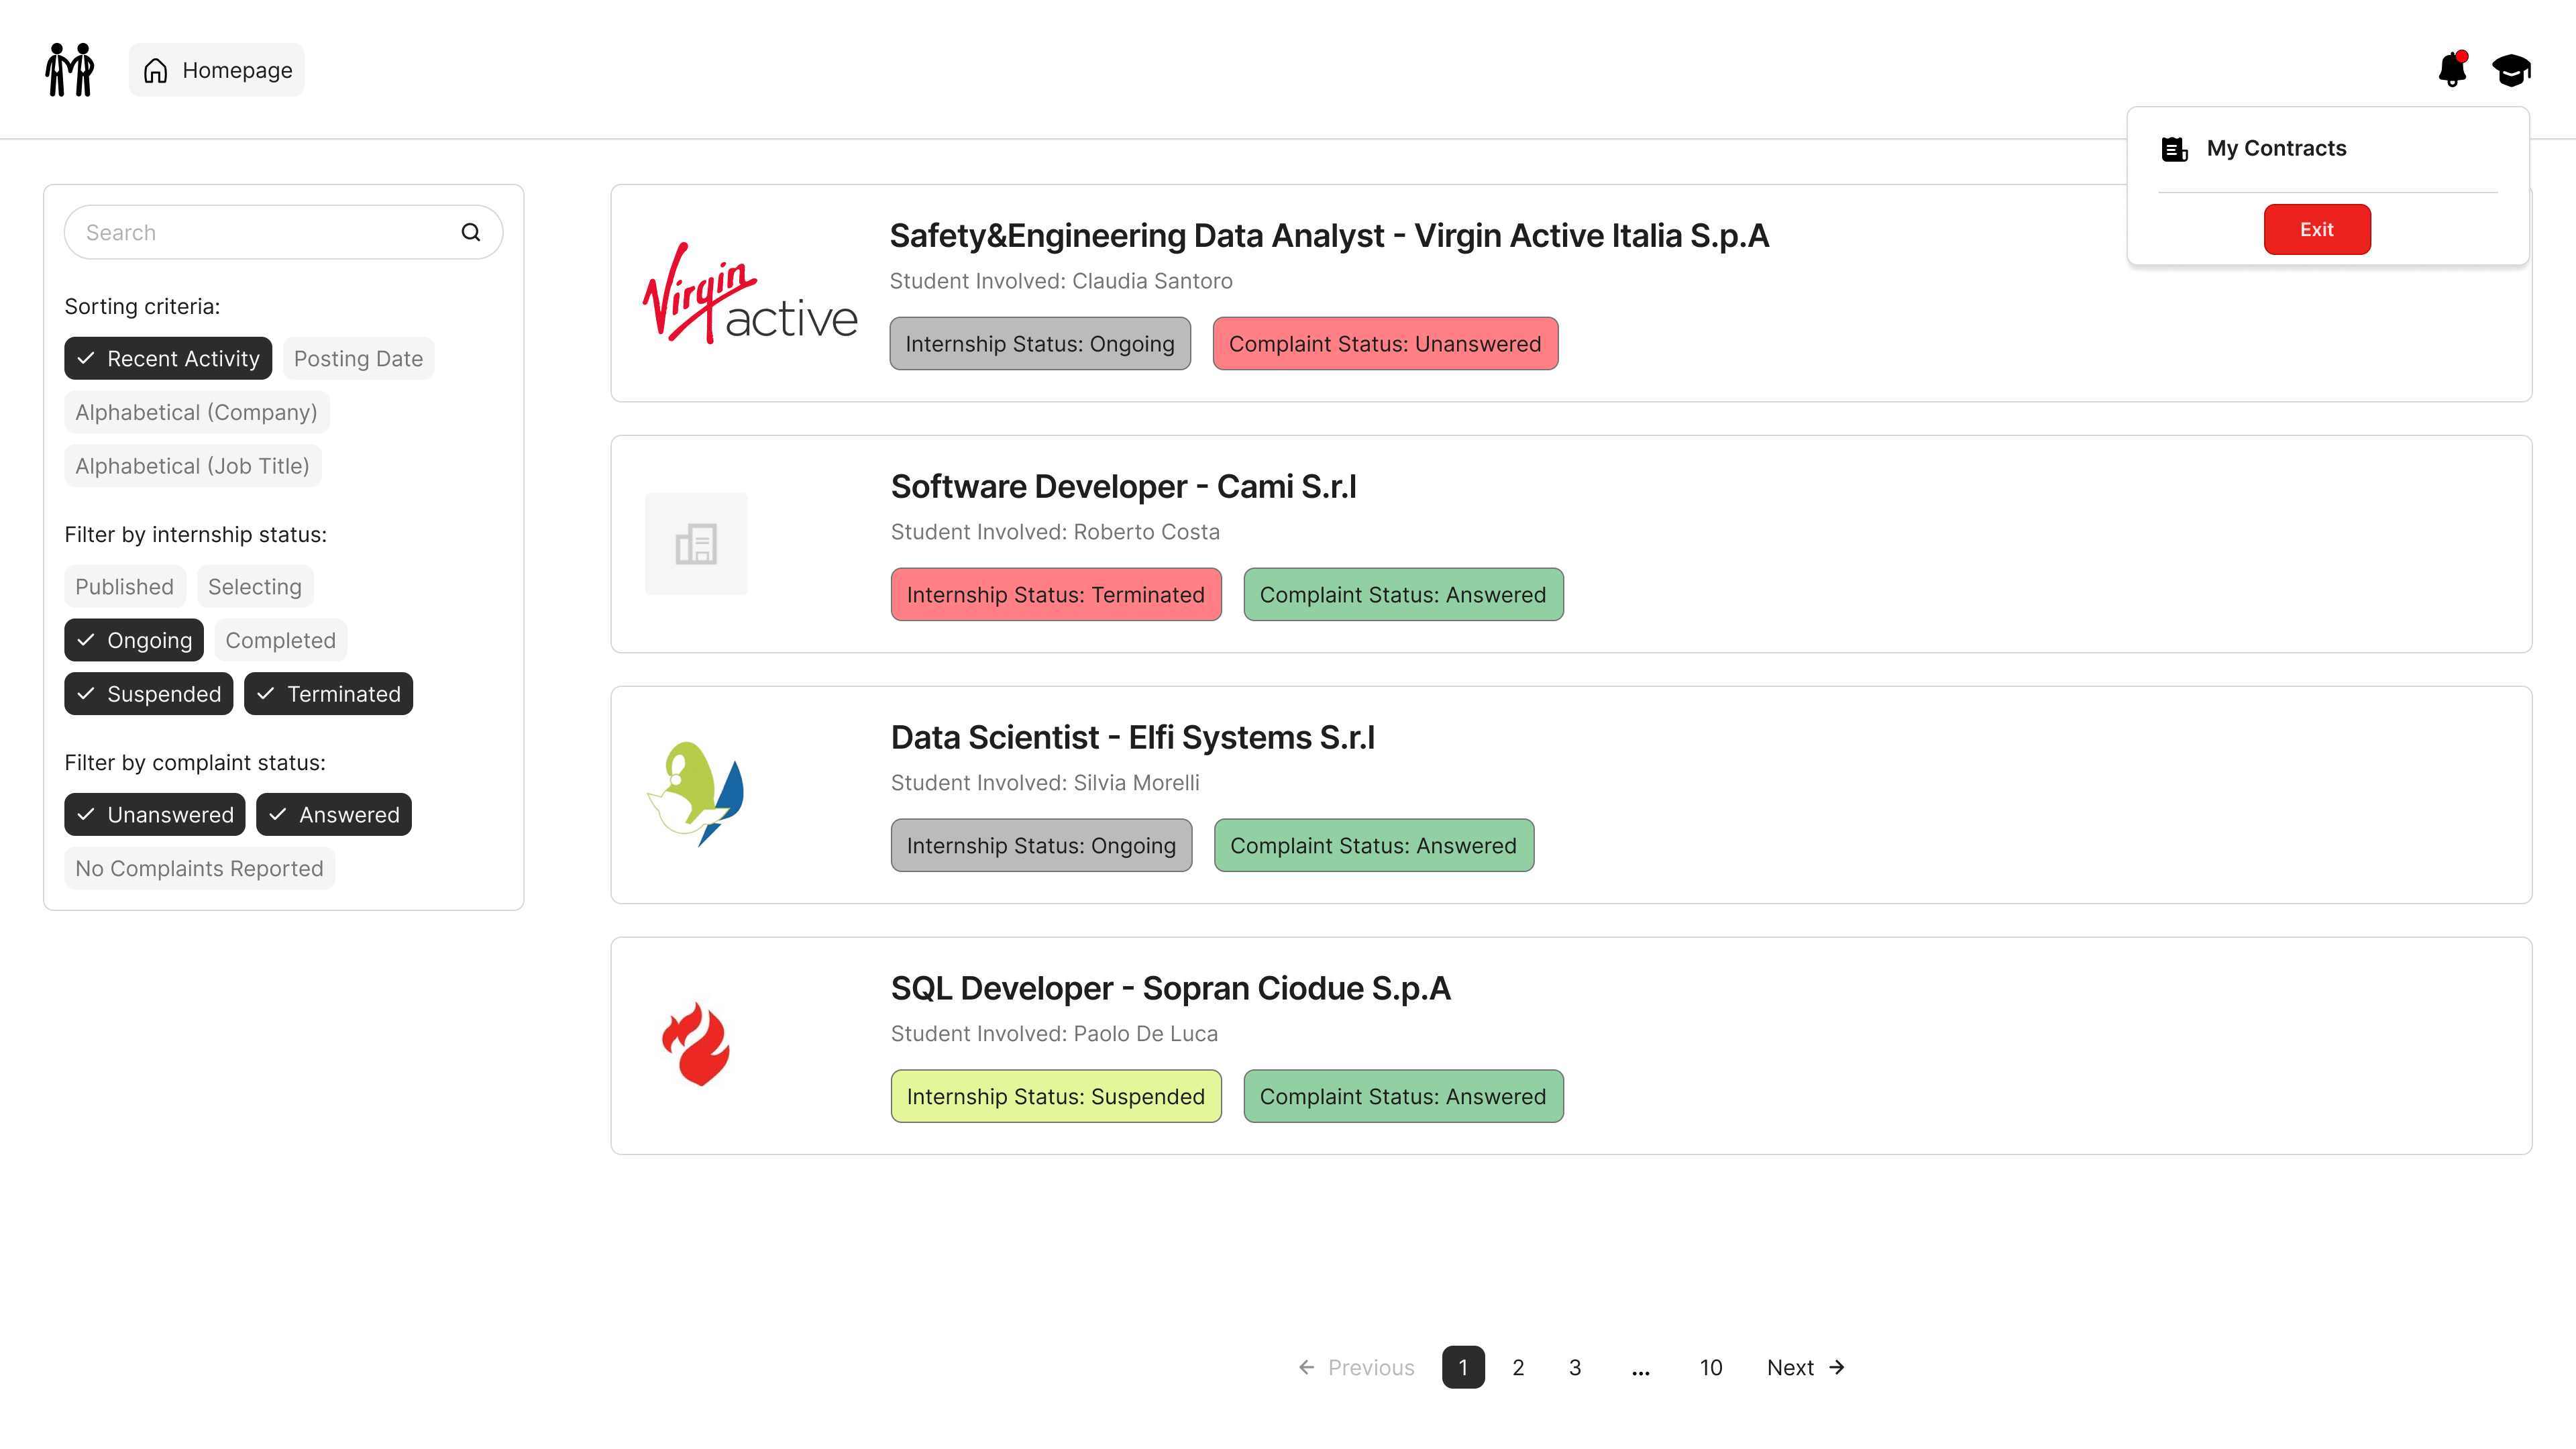
\includegraphics[width=1.0\textwidth]{Images/GUI/UN/Homepage - Contract - UN.png}}
    \caption{Homepage - UN - Notification}
    \label{fig:homepage-un-notification}
\end{figure}

\section{"My Contracts" - UN}
\label{subsec:my-contracts-un}%

\begin{figure}[H]
    \centering
    \fbox{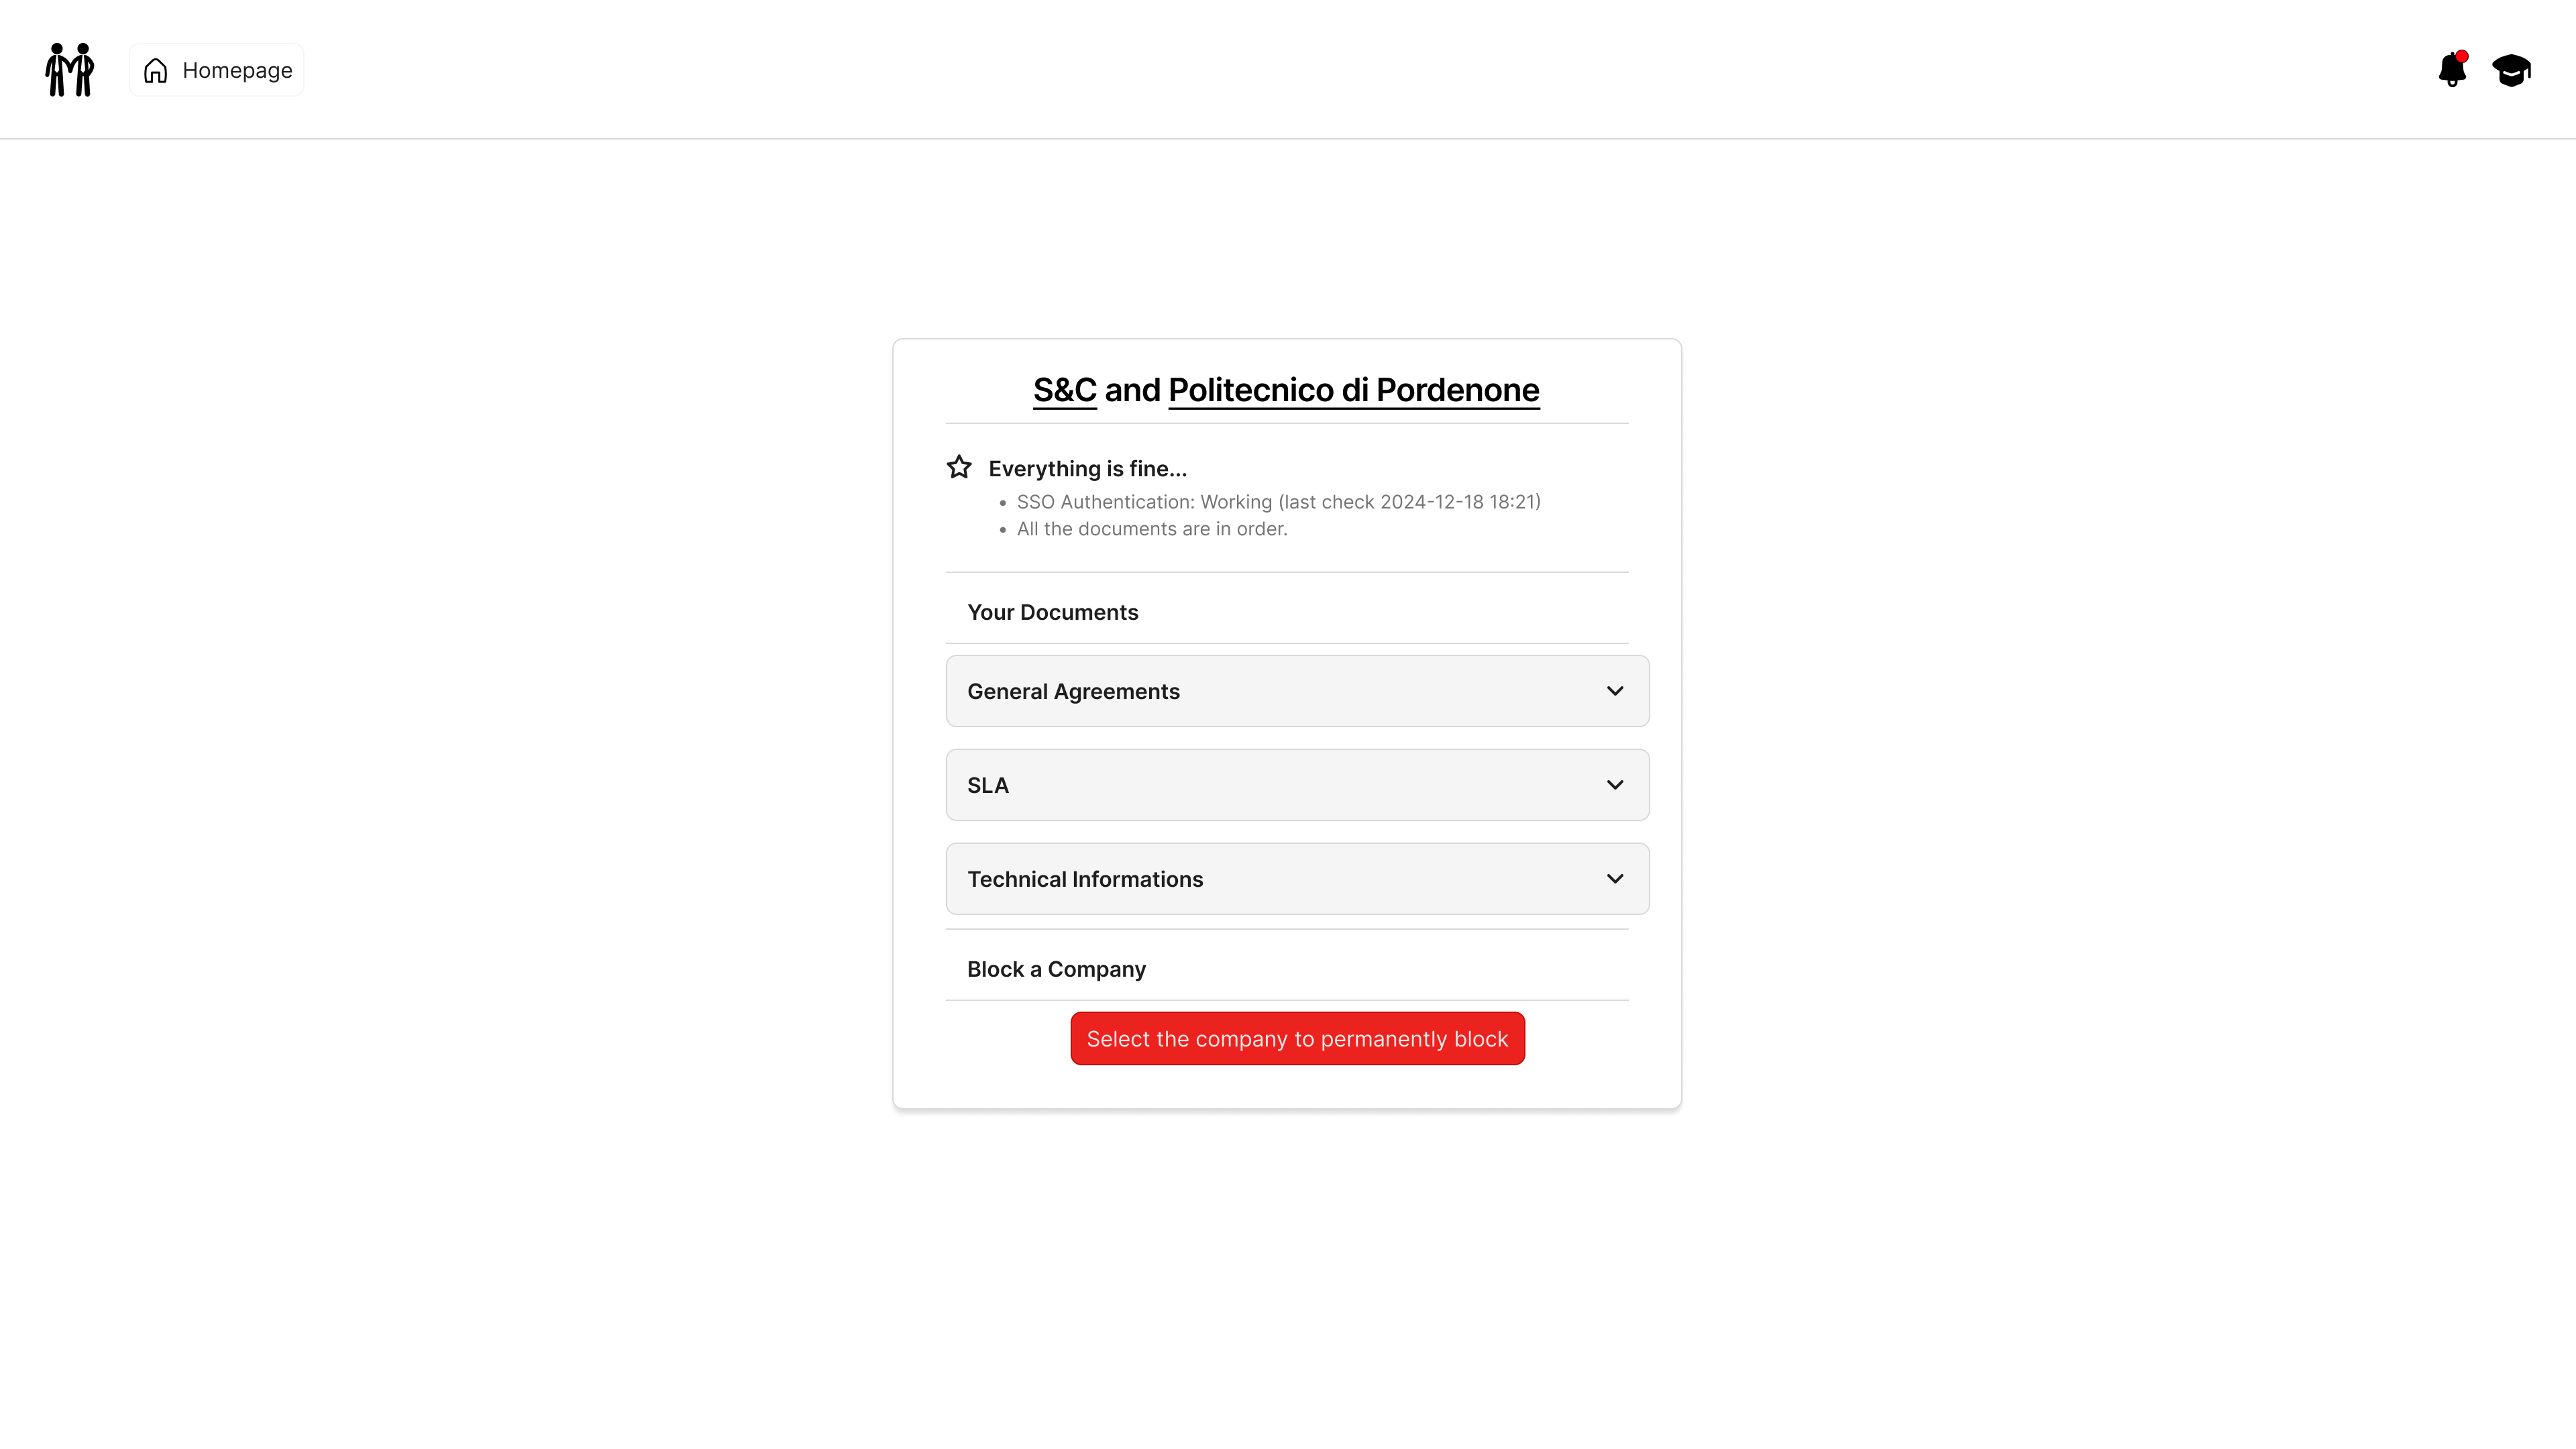
\includegraphics[width=1.0\textwidth]{Images/GUI/UN/My Contracts - UN.png}}
    \caption{"My Contracts" - UN}
    \label{fig:my-contracts-un}
\end{figure}

\par The "My Contracts" page allows the UN to view all the contracts that exist between the university and S\&C as well
as block a malicious company. The page also provides a status check for the connection between the university's SSO
service and S\&C.

\begin{figure}[H]
    \centering
    \fbox{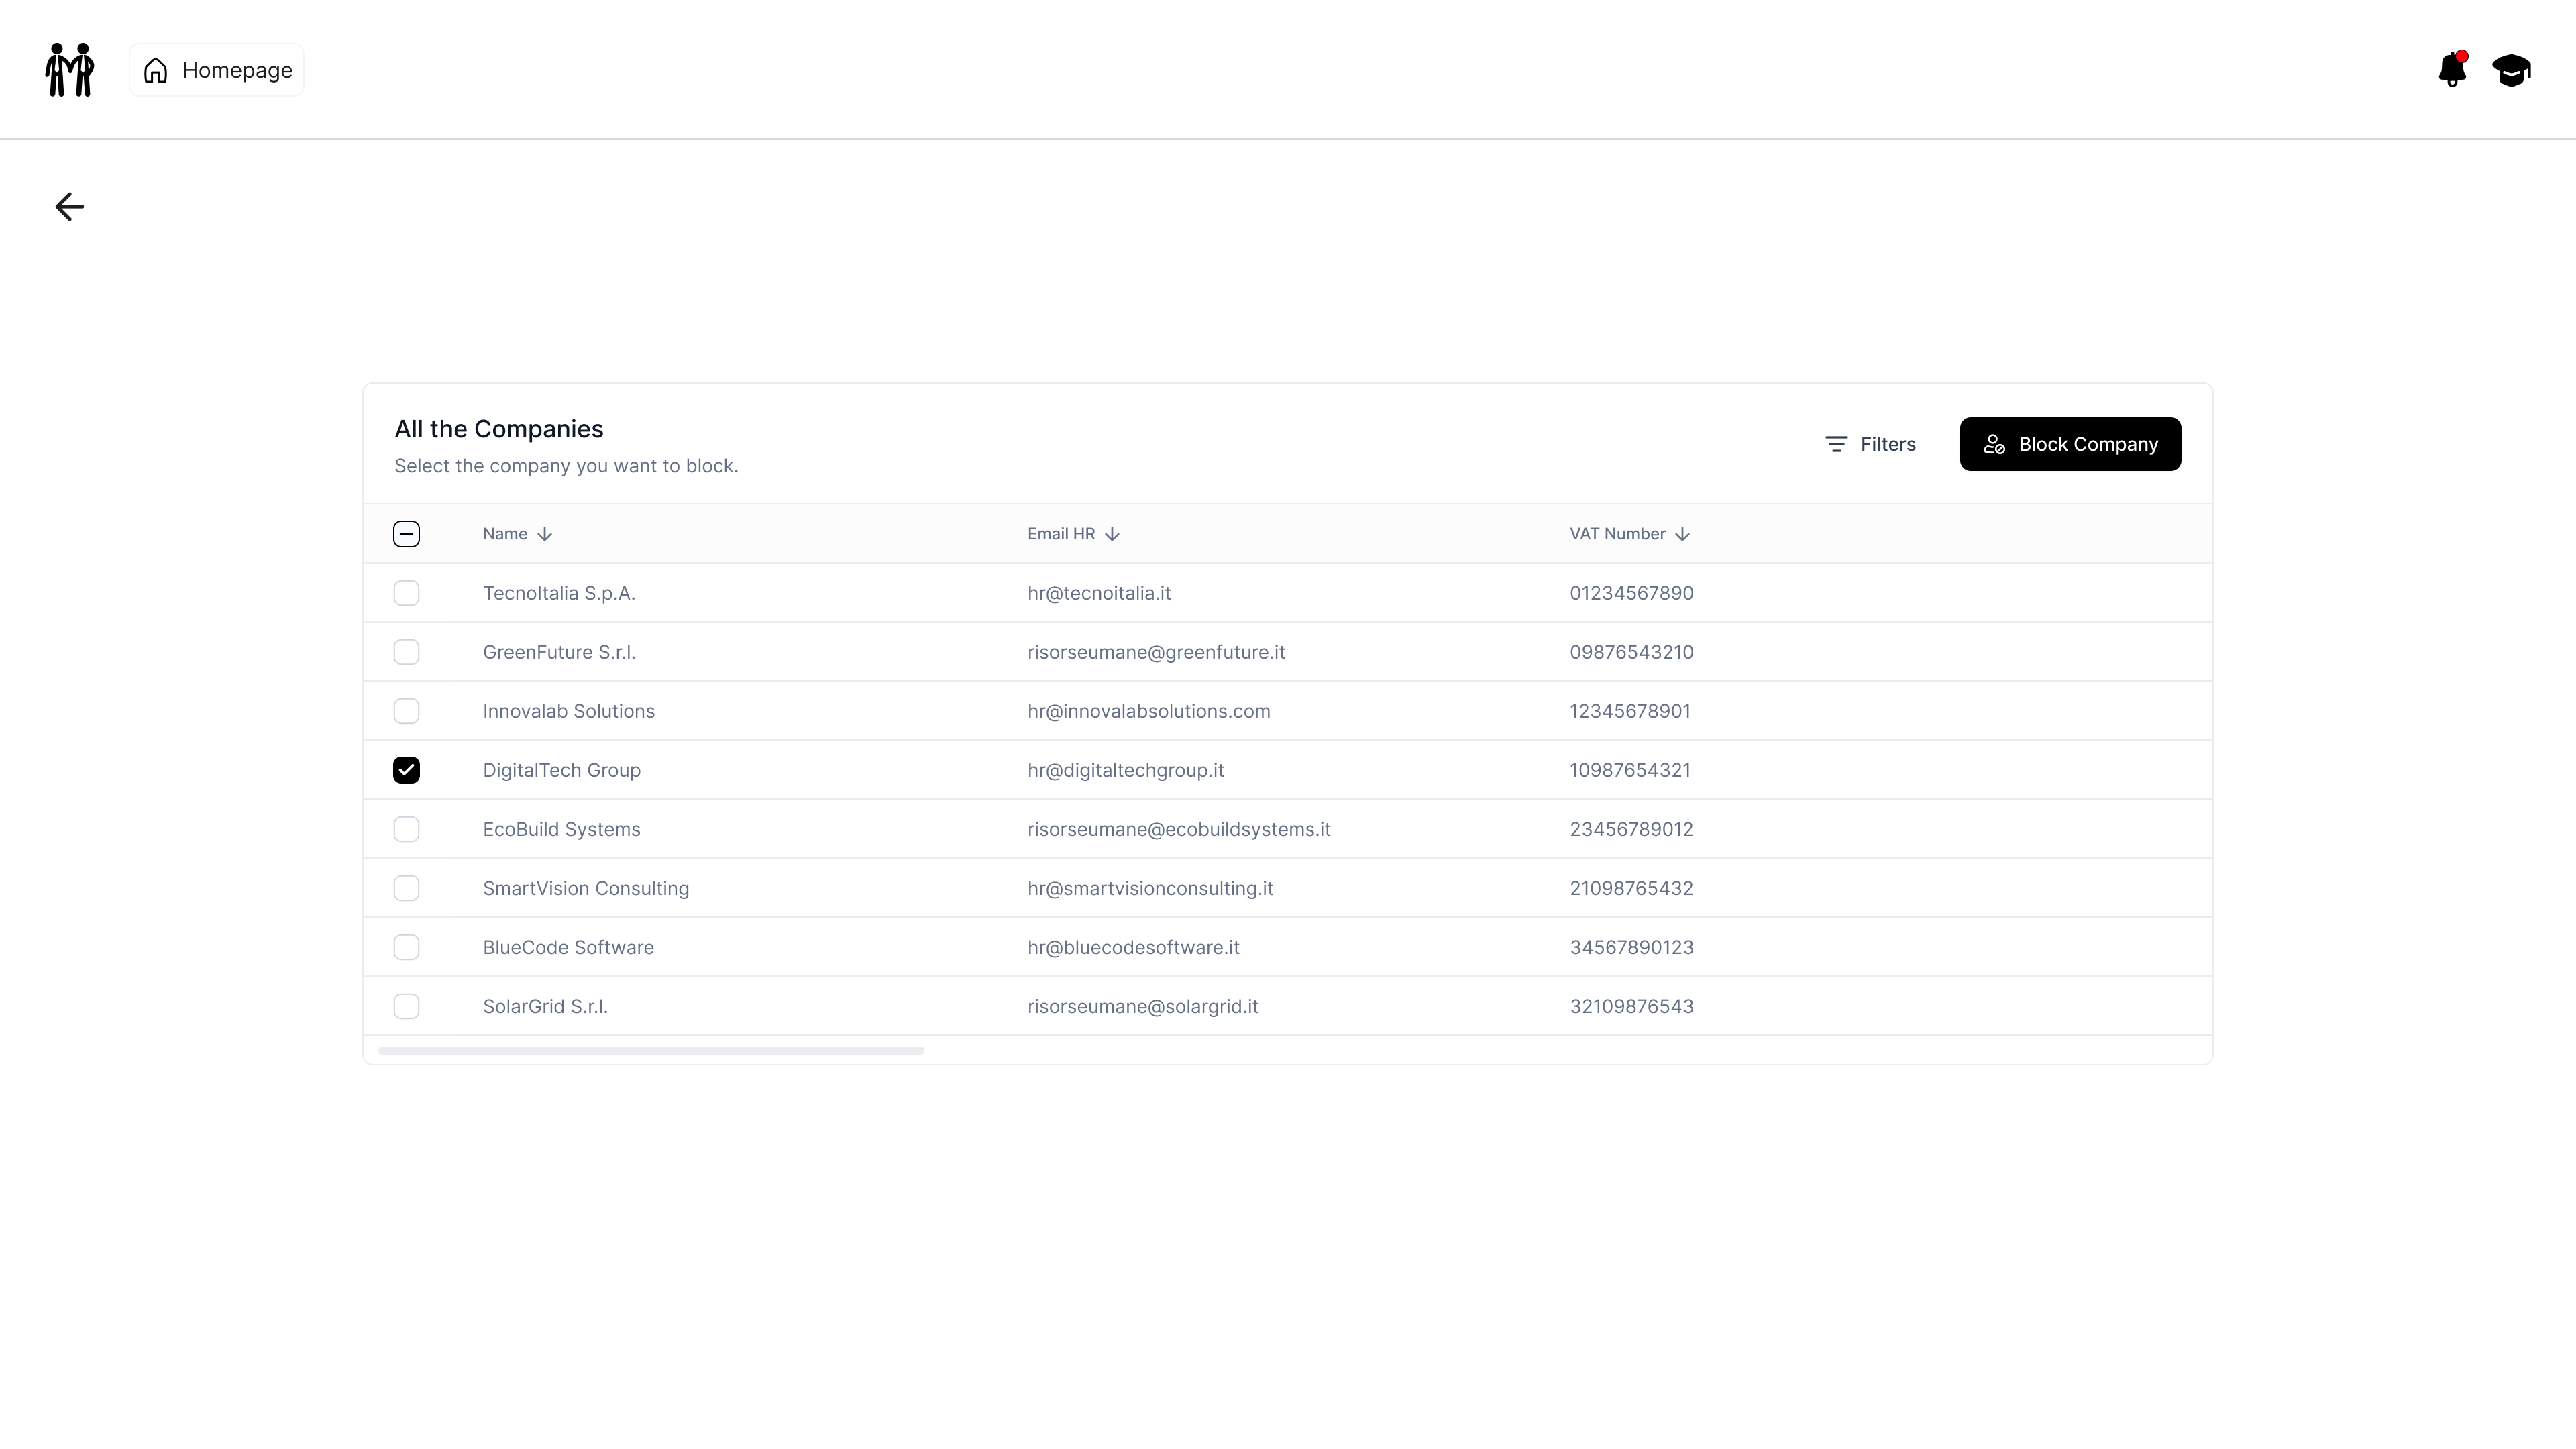
\includegraphics[width=1.0\textwidth]{Images/GUI/UN/Block CO Selection - UN.png}}
    \caption{Block CO Selection - UN}
    \label{fig:block-co-selection-un}
\end{figure}

\par The "Block CO Selection" page allows the UN to block a malicious company. The UN can search for the company using
the filters provided and then block it.

\subsection{Internship Details - UN}
\label{subsec:internship-details-un}%

\begin{figure}[H]
    \centering
    \fbox{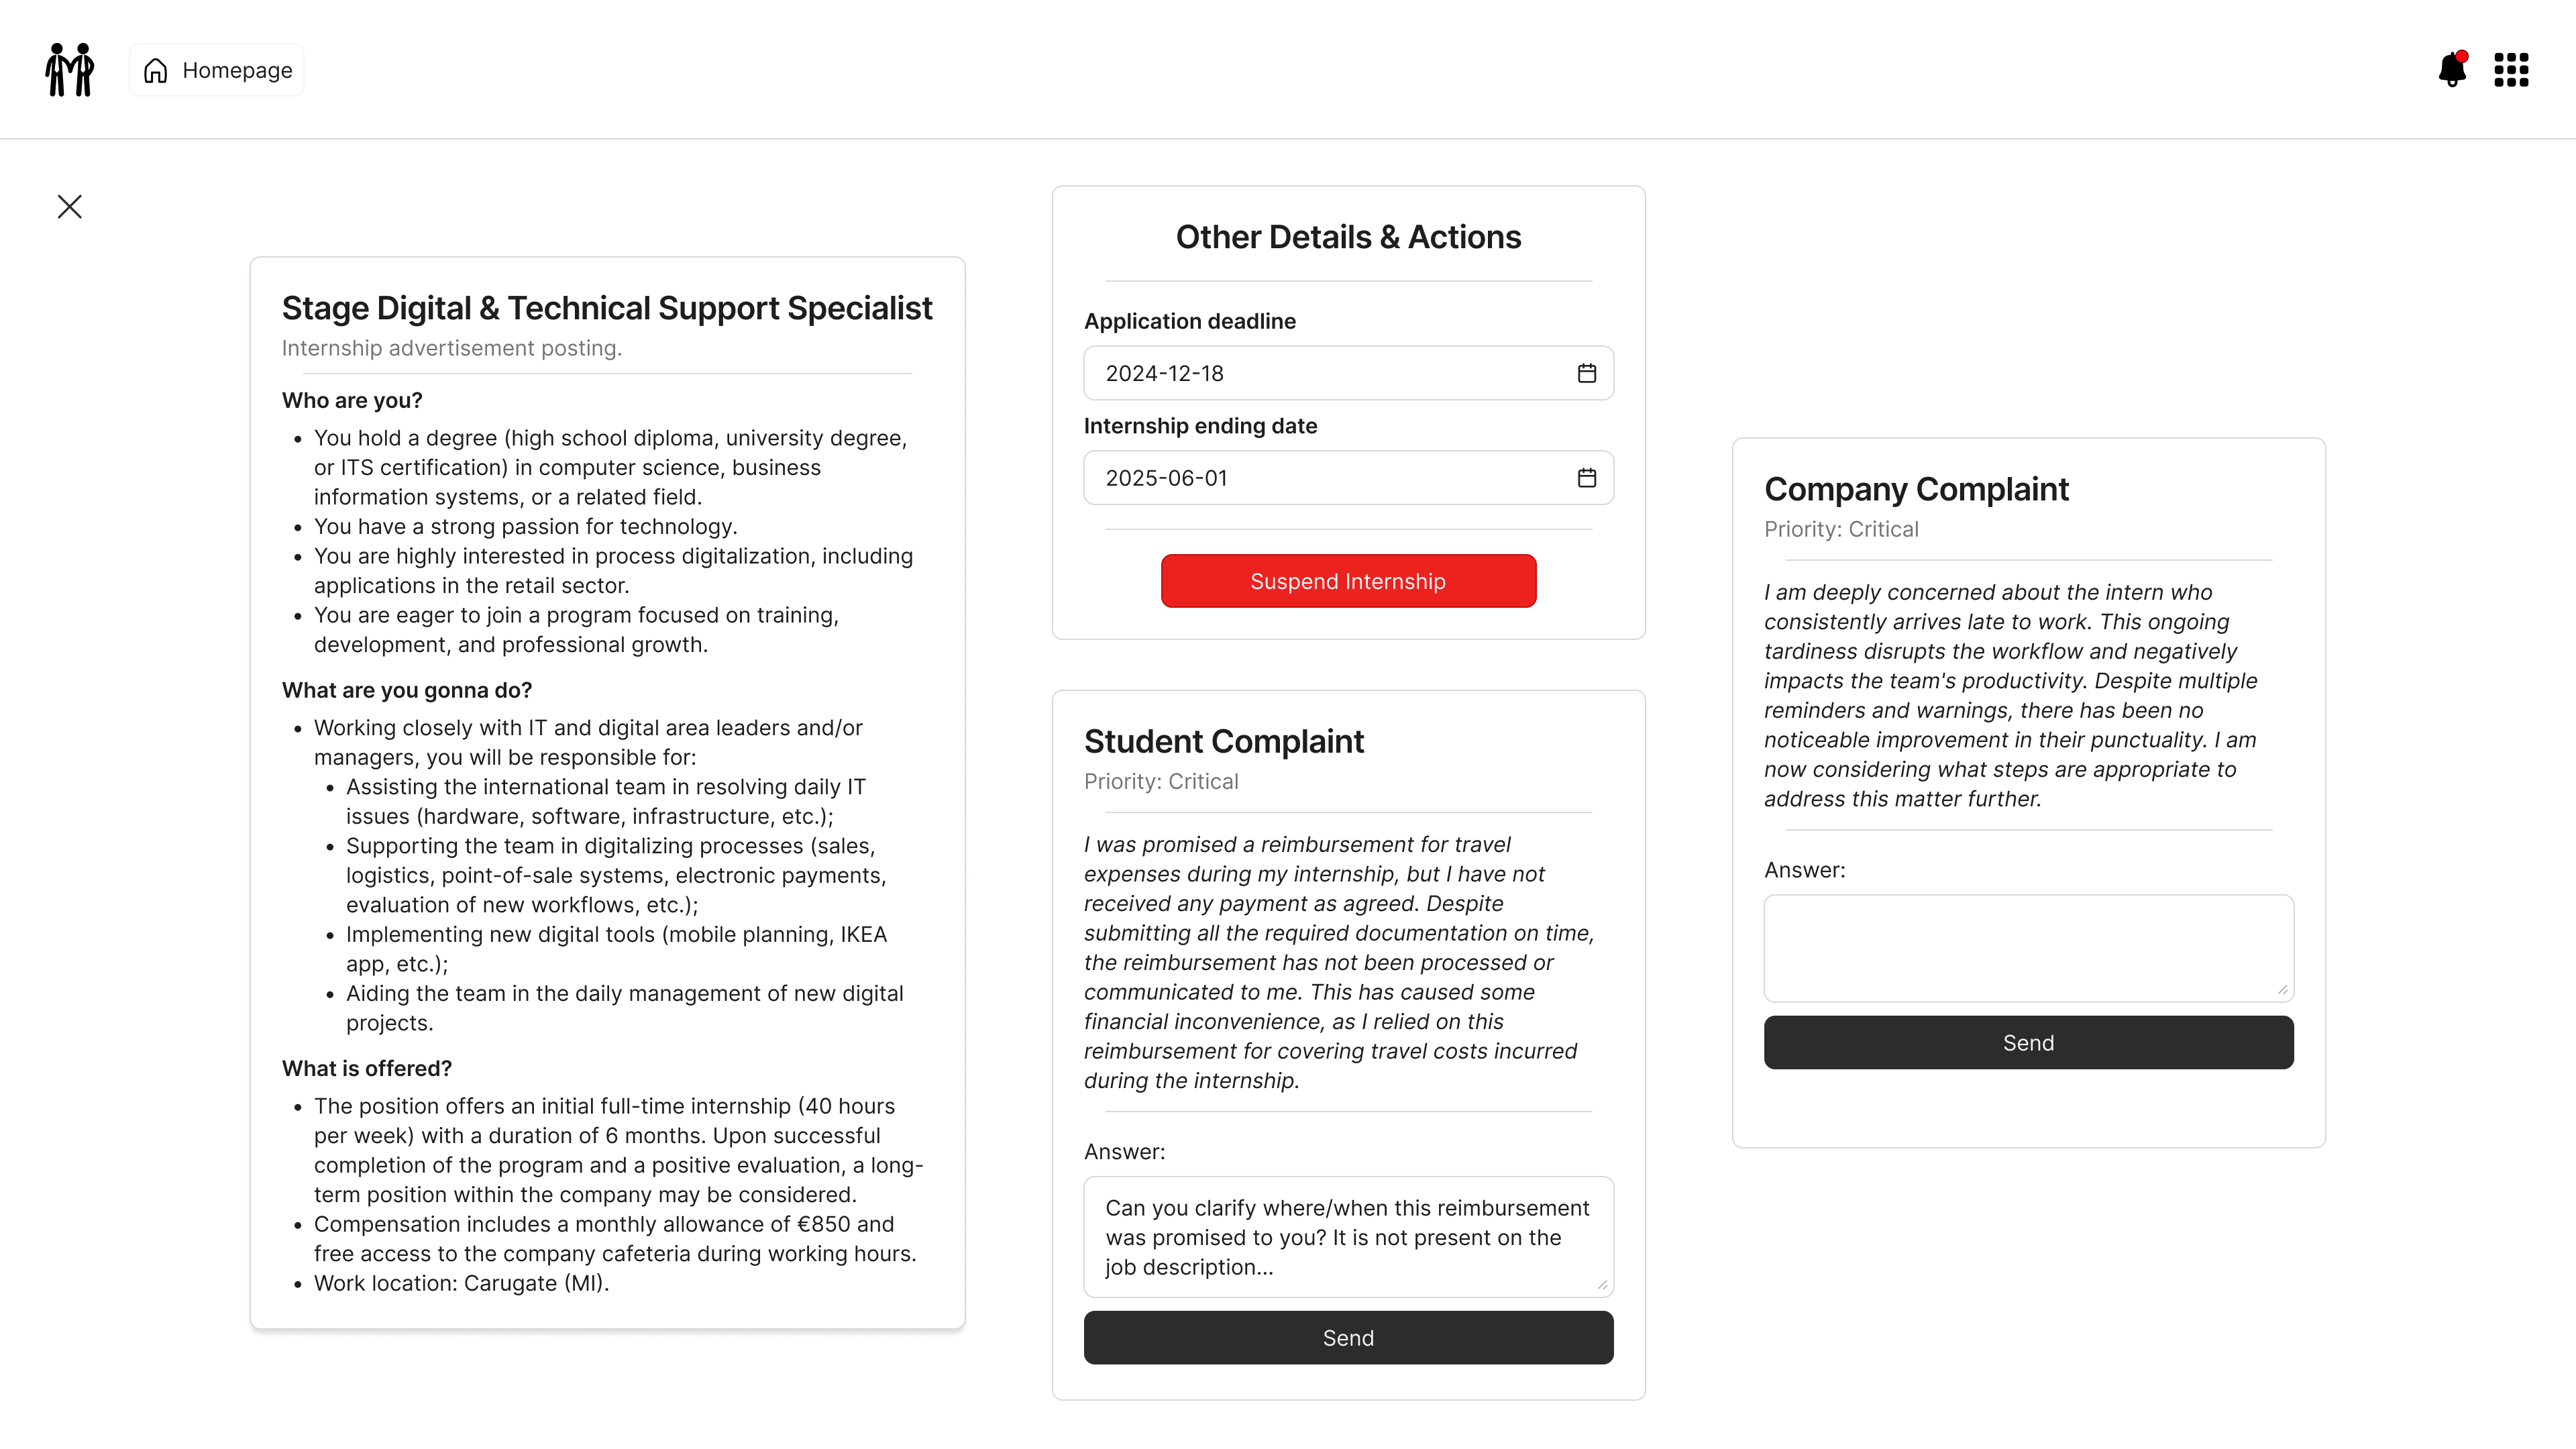
\includegraphics[width=1.0\textwidth]{Images/GUI/UN/Internship Details - UN.png}}
    \caption{Internship Details - UN}
    \label{fig:internship-details-un}
\end{figure}

\par The Internship Details page allows the UN to view all the details of an internship. The UN can view and answer to
eventual complaints and, if needed, suspend the internship.
